% Synchronized to r29817
\include{fli4l}

\makeindex

\begin{document}

\newcommand{\titlename}{fli4l -- flexible internet router for linux}

\flhypersetup{pdftitle=\titlename}
\pdfbkmrk{-1}{\titlename}{title}
\title{\titlename\\ Version \version}

\author{Frank Meyer\\ \email{frank@fli4l.de} \and L'équipe fli4l\\ \email{team@fli4l.de}}

\maketitle
\pdfbkmrk{0}{\contentsname}{table}
\tableofcontents

% Synchronized to r29819
% Last Update: $Id$
\chapter{Dokumentation des Basispaketes}

\section{Einleitung}

fli4l ist ein auf Linux basierender ISDN-, DSL-, UMTS- und Ethernet-Router mit
geringen Anforderungen an die zugrunde liegende Hardware: Ein USB-Stick als
Bootmedium, ein Intel Pentium MMX-Prozessor, 64 MiB RAM sowie (mindestens) eine
Ethernet-Netzwerkkarte sind dafür vollkommen ausreichend. Das notwendige
Bootmedium kann unter Linux, Mac OS~X oder MS~Windows erstellt werden. Dabei sind keine
Linux-Kenntnisse erforderlich, aber durchaus hilfreich. Grundkenntnisse von
Netzwerken, TCP/IP, DNS und Routing sollten jedoch vorhanden sein. Für eigene
Erweiterungen/Entwicklungen, welche über die Standardkonfiguration hinausgehen,
sind ein lauffähiges Linux-System und Linux-Kenntnisse notwendig.

fli4l unterstützt verschiedene Bootmedien, darunter USB-Sticks, Festplatten,
CDs und nicht zuletzt das Booten über das Netzwerk. Ein USB-Stick ist in
vielerlei Hinsicht ideal: Heutzutage kann so gut wie jeder PC von einem
USB-Stick starten, er ist recht erschwinglich, er hat eine ausreichende Größe,
und man kann sowohl unter Linux als auch unter MS~Windows auf relativ einfache
Weise eine fli4l-Installation darauf ablegen. Auch ist er im Gegensatz zu einer
CD beschreibbar und kann somit nichtflüchtige Konfigurationsdaten (wie z.B.
DHCP-Leases) speichern.

\begin{itemize}

\item Allgemeine Features

\begin{itemize}
\item Erstellen von Bootmedien unter \jump{sec:bootmedien_linux}{Linux},
      \jump{sec:bootmedien_linux}{Mac OS~X} und
      \jump{sec:bootmedien_windows}{MS~Windows}
\item Konfiguration über normale ASCII/UTF-8-Dateien
\item Unterstützung von IP-Masquerading und Portweiterleitung
\item Least-Cost-Routing (LCR): automatische Auswahl des Providers, je nach
      Uhrzeit
\item Anzeige/Berechnung/Protokollierung von Verbindungszeiten und -kosten
\item MS~Windows/Linux-Client imonc mit Schnittstelle zu imond und telmond
\item Upload von aktualisierten Konfigurationsdateien über MS~Windows-Client
      imonc oder via SCP unter Linux
\item Bootmedien nutzen das VFAT-Dateisystem zum dauerhaften Speichern von
      Dateien
\item Paketfilter: Protokollieren von Zugriffen von außen auf gesperrte Ports
\item Einheitliche Abbildung von WAN-Schnittstellen auf sogenannte Circuits
\item Paralleler Betrieb von ISDN- und DSL/UMTS-Circuits ist möglich
\end{itemize}

\item Router-Basisfunktionalität

\begin{itemize}
\item Linux-Kernel 3.18 oder 3.19
\item Paketfilter und IP-Masquerading
\item DNS-Server, um die Anzahl von DNS-Abfragen an externe DNS-Server zu
      reduzieren
\item Netzwerkfähiger imond-Server mit Monitor- und LCR-Steuerfunktionen
\item Netzwerkfähiger telmond-Server zur Protokollierung von eingehenden
      Telefonanrufen
\end{itemize}

\item Ethernet-Unterstützung

\begin{itemize}
\item Aktuelle Netzwerkkartentreiber: Unterstützung von über 140 Kartentypen
\end{itemize}

\item DSL-Unterstützung

\begin{itemize}
\item Roaring Penguin PPPoE-Treiber, mit Dial-on-Demand (abschaltbar)
\item PPTP für DSL-Anbindungen in Österreich und den Niederlanden
\end{itemize}

\item ISDN-Unterstützung

\begin{itemize}
\item Unterstützung von knapp 60 ISDN-Kartentypen
\item Mehrere ISDN-Verbindungsmöglichkeiten: eingehend/ausgehend/Rückruf,
      "`roh"'/Punkt-zu-Punkt (ppp)
\item Kanalbündelung: automatische Bandbreitenanpassung oder manuelle
      Zuschaltung des zweiten Kanals über MS~Windows-/Linux-Client
\end{itemize}

\item Optionale Programmpakete

\begin{itemize}
\item DNS-Server
\item DHCP-Server
\item SSH-Server
\item Einfache Online/Offline-Anzeige über LED
\item Serielle Konsole
\item Mini-Webserver für ISDN- und DSL-Monitoring sowie zur Rekonfiguration
      und/oder Aktualisierung des Routers
\item Zugangserlaubnis für bestimmte konfigurierte Netzwerke von außen
\item Unterstützung für PCMCIA-Karten (heutzutage PC-Cards genannt)
\item Protokollierung von Systemmeldungen
\item Konfiguration von ISAPnP-Karten mit den isapnp-Werkzeugen
\item Zusätzliche Werkzeuge zum Debugging
\item Konfiguration der seriellen Schnittstelle
\item Notfallsystem zur Fernwartung über ISDN
\item Software zur Anzeige konfigurierbarer Informationen auf einem LCD, z.B.
      von Übertragungsraten, CPU-Auslastung etc.
\item PPP-Server/Router über serielle Schnittstelle
\item ISDN-Modem-Emulator über serielle Schnittstelle
\item Druckerserver
\item Synchronisierung der Uhrzeit mit externen Zeit-Servers
\item Ausführen von benutzerdefinierten Kommandos bei eingehenden Telefonanrufen
      (z.B. um ein Internet-Einwahl durchzuführen)
\item Unterstützung von IP-Aliasing (mehrere IP-Adressen pro
      Netzwerkschnittstelle)
\item VPN-Unterstützung
\item IPv6-Unterstützung
\item WLAN-Unterstützung: fli4l kann sowohl Zugangsknoten als auch Client sein
\item RRD-Tool zum Überwachen des fli4l
\item und vieles andere mehr\ldots
\end{itemize}

\item Hardwarevoraussetzungen

\begin{itemize}
\item Intel Pentium-Prozessor mit MMX Unterstützung
\item 64 MiB Speicher, besser 128 MiB
\item Ethernet-Netzwerkkarte
\item ISDN: unterstützte ISDN-Karte
\item ein USB-Stick, eine ATA-Festplatte oder eine CF-Karte (die genauso wie
      eine ATA-Festplatte angesprochen wird); alternativ ist auch der Start von
      CD möglich
\end{itemize}

\item Softwarevoraussetzungen

Unter Linux werden folgende Programme vorausgesetzt:

\begin{itemize}
\item GCC und GNU make
\item syslinux
\item mtools (mcopy)
\end{itemize}

Unter MS~Windows werden keine zusätzlichen Werkzeuge benötigt, fli4l bringt
alles Notwendige mit.

\end{itemize}

Zusätzlich gibt es zur Steuerung/Statusanzeige des fli4l-Routers noch
den Client imonc. Dieses Programm ist für MS~Windows (windows/imonc.exe)
und auch für Linux (unix/gtk-imonc) vorhanden.

Und nun \ldots \bigskip

Viel Spaß mit fli4l!\bigskip

Frank Meyer und das fli4l-Team 

\email{team@fli4l.de}

% Do not remove the next line
% Synchronized to r30469

\chapter{Installation et configuration}

\section{Décompacter les archives}

Sous Linux~:

\begin{verse}\texttt{tar xvfz fli4l-\version.tar.gz}\end{verse}

\noindent Si cela ne fonctionne pas, essayez la procédure suivante~:

\begin{verse}\texttt{gzip -d < fli4l-\version.tar.gz | tar xvf -}\end{verse}

Pour ceux qui veulent installer fli4l dans un répertoire existant, ils doivent
utiliser le script \texttt{mkfli4l.sh -c} avant l'installation~:

\begin{verse}
    \texttt{cd fli4l-\version}\\
    \texttt{sh mkfli4l.sh -c}
\end{verse}

Il est toutefois recommandé d'utiliser un nouveau répertoire pour chaque nouvelle
version~-- la configuration peut être prise en charge très simplement avec un
outil servant à la comparaison des fichiers.

Sous Windows, l'archive de compression .tar peut être extraite, par exemple,
avec WinZip. Il faut faire attention que les fichiers dans les sous-répertoires
soient {\emph bien} décompressés (voir les paramètres dans Winzip~!). Il faut
vérifier que l'option "Smart TAR CR conversion" est décochée dans
{\emph Options \pfeil Configuration}. Si cette option est cochée il peut y avoir
quelques erreurs (plus ou moin important) à l'extraction des fichiers.

7-Zip (\altlink{http://www.7-zip.org/}) est un programme alternatif, il est
aussi puissant que WinZip et en plus il est open source, je vous le recommande.

Les fichiers suivants sont installés dans le sous-répertoire \texttt{fli4l-\version/}~:

\begin{itemize}
\item Documentation~:
  \begin{itemize}
  \item doc/deutsch/* Documentation Allemande
  \item doc/english/* Documentation Anglaise
  \item doc/french/* Documentation Française
  \end{itemize}

\item Configuration~:
  \begin{itemize}
  \item config/*.txt Fichiers de configurations, ils doivent être adaptés
  \end{itemize}

\item Scripts/Procédures~:
  \begin{itemize}
  \item mkfli4l.sh création du média de boot pour les fichiers configurés~:
    Version-Linux/Unix
  \item mkfli4l.bat création du média de boot pour les fichiers configurés~:
    Version-Windows
  \end{itemize}

\item Kernel/Fichier de boot~:
  \begin{itemize}
  \item img/kernel Linux-Kernel
  \item img/boot*.msg texte avec écran de démarrage
  \end{itemize}

\item Paquetage supplémentaire~:
  \begin{itemize}
  \item opt/*.txt Ces fichiers décrivent, la direction des programmes source
    et de configuration pour l'archive OPT.img.
  \item opt/... Optionnel Module-Kernel, fichiers et programmes.
  \end{itemize}

\item Code source~:
  \begin{itemize}
  \item src/* Code source/outils pour Linux, voir src/README
  \end{itemize}

\item Programme~:
  \begin{itemize}
  \item unix/mkfli4l* Création du disque de Boot~: Version-Unix/Linux
  \item windows/* Création du disque de Boot~: Version-Windows
  \item unix/imonc* client-imond pour Unix/Linux
  \item windows/imonc/* client-imond pour Windows
  \end{itemize}
\end{itemize}


\section{Configuration}

\subsection{Éditer les fichiers de configurations}

Pour configurer fli4l, vous devez paramétrez dans config/*.txt les fichiers.
Il est recommandé pour pouvoir comparer par la suite sa configuration ou pour
pouvoir gérer plusieurs configurations, de créer une copie du répertoire config
et d'effectuer la configuration dans cette copie. La comparaison des fichiers
de configurations sera alors possible au moyen d'outil approprié (par ex. "diff"
sous *nix) est relativement facile. Supposons que votre copie de config se trouve
dans le répertoire "ma\_config", vous devez d'abord aller dans le répertoire
fli4l et utiliser la commande~:

\begin{example}
\begin{verbatim}
    ~/src/fli4l> diff -u {config,ma_config}/build/rc.cfg | grep '^[+-]'
    --- config/build/rc.cfg    2007-03-22 15:34:39.085103706 +0100
    +++ ma_config/build/rc.cfg        2007-03-22 15:34:31.094317441 +0100
    -PASSWORD='/P6h4iOIN5Bbc'
    +PASSWORD='3P8F3KbjYgzUc'
    -NET_DRV_1='ne2k-pci'
    +NET_DRV_1='pcnet32'
    -START_IMOND='no'
    +START_IMOND='yes'
    -OPT_PPPOE='no'
    +OPT_PPPOE='yes'
    -PPPOE_USER='anonymer'
    -PPPOE_PASS='surfer'
    +PPPOE_USER='moi'
    +PPPOE_PASS='mon mot de passe'
    -OPT_SSHD='no'
    +OPT_SSHD='yes'
\end{verbatim}
\end{example}

On voit très bien ici, les différents paramètres qui sont configurés pour un
simple routeur-DSL, même si à première vue le fichier de configuration effraye
avec ca profusion de réglages.

\subsection{Configuration via un fichier de configuration spéciale}

La configuration se répartit sur différents fichiers avec le concept de module,
le travaille devient parfois un peut laborieux, on peut placer les fichiers de
configuration dans un fichier unique \emph{$<$liste~config$>$/\_fli4l.txt}
Il est plus facile de lire ou comparer son contenu que d'ouvrir la liste des
fichiers *.txt un par un, mais l'on doit quand même configurer et garder les
fichiers originaux pour la construction de fli4l. Pour rester sur l'exemple
mentionné ci-dessus, on peut configurer un simple routeur-DSL dans ce fichier~:

\begin{example}
\begin{verbatim}
    PASSWORD='3P8F3KbjYgzUc'
    NET_DRV_N='1'
    NET_DRV_1='pcnet32'
    START_IMOND='yes'
    OPT_PPPOE='yes'
    PPPOE_USER='moi'
    PPPOE_PASS='mon mot de passe'
    OPT_SSHD='yes'
\end{verbatim}
\end{example}

Vous devez éviter de mélanger différente version de configuration.

\subsection{Variables}

  Vous remarquerez que certaines variables sont commentées. Si c'est le cas, ils
  sont réduit à une information raisonnable. Cette attribution par défaut est
  documentée pour chaque variable. Si vous souhaitez insérer un autre commentaire
  pour cette variable, vous devez supprimer le commentaire et définir le votre,
  vous devez garder la caractère ('\#') au début du commentaire.


\marklabel{VARIANTEN}{\section{Procédures d'installation}}

Dans les versions précédentes, la seule option pour fli4l était de démarrer
sur une disquette. Maintenant, ce n'est plus possible pour les raisons
mentionnée ci-dessus, en alternatif vous pouvez utiliser une clé USB.

Maintenant vous pouvez démarrer sur d'autre média comme par exemple (CD,
HD, Réseau, Compact-Flash, DoC, \ldots), fli4l peut être installé sur
divers médias (HD, Compact-Flash, DoC). En plus, fli4l peut être démarré de
trois manières différentes~:

\begin{description}
\item [Single Image] Le Bootloader (ou chargeur automatique) charge le noyau
  Linux ensuite, fli4l est dans une seule image, ainsi fli4l peut être lancé
  sans avoir accés à aucun média de boot. Exemples d'utilisation pour les
  différents types de boot \emph{integrated}, \emph{attached}, \emph{netboot} et \emph{cd}.
\item [Split Image] Le Bootloader charge le noyau Linux, dans une première étape
  l'image rudimentaire de fli4l configure et monte sur le média. Dans une
  deuxième étape les fichiers restants sont chargés dans ce média à partir
  du média de boot. Exemple d'utilisation pour les différents types
  de boot \emph{hd (Typ A)}, \emph{ls120}, \emph{attached}, \emph{cd-emul}.
\item [Installation Medium] Le Bootloader charge le noyau Linux ensuite l'image
  rudimentaire de fli4l installe les fichiers systèmes sur le média existant,
  il n'a pas besoin de décompresser d'autre archive. Exemple pour une installation
  de disque dur avec le type B
\end{description}

Vous devez d'abord installer fli4l une fois dans la version minimale et ainsi
acquérir de expériences. Ensuite vous pourrez utiliser fli4l comme un répondeur
téléphonique ou comme un Proxy-HTTP. Vous avez ainsi l'avance d'avoir l'expérience
d'avoir un routeur essentiel qui fonctionne.

Pour l'installation, nous distinguons au total quatre versions~:

\begin{description}
\item[Clé-USB] Le routeur sur une clé-USB
\item[Lecteur-CD] Le routeur sur un CD
\item[réseau] pour booter sur le réseau filaire
\item[Installation-HD Typ A] routeur sur un disque dur, CF, DoC~-- avec une
  seul partition FAT
\item[Installation-HD Typ B] routeur sur un disque dur, CF, DoC~-- avec une
  partition FAT et une partitions ext3
\end{description}


\marklabel{INSTALLTYP0}{\subsection{Routeur sur une clé USB}}

Linux traite les clés USB comme des disques durs, donc les explications sont
les mêmes que pour une installation sur un disque dur. Notez s'il vous plaît,
que les pilotes en fonction du port USB doivent être chargées avec \var{OPT\_\-USB}
pour accéder à la clé USB puis avec \var{OPT\_\-HDINSTALL} pour l'installation 


\marklabel{INSTALLTYP0}{\subsection{Routeur sur CD ou par le réseau}}

Tous les fichiers nécessaires se trouvent sur le média de boot et décompacté
dans un disque RAM dynamique. Dans une configuration minimale le routeur fli4l
a besion de seulement 64 Mio RAM. Pour une configuration maximale le routeur est
limitée que par la capacité du média de boot et la mémoire principale installé.


\marklabel{INSTALLTYPA}{\subsection{Type A~: Routeur sur disque dur~-- Une seule partition FAT}}

C'est la même installation qu'avec la version CD, sauf que les fichiers sont stockés
sur un disque dur. Quand nous employons le terme \flqq{}Disque dur\frqq{} cela signifie
également d'autres dispositifs comme, un compacts flash de 8 Mio et d'autres
dispositifs que Linux peut traiter comme un disque dur. Depuis la version 2.1.4
fli4l peut utiliser le DiskOnChip mémoire flash de M-System et le disque SCSI.

La taille de l'archive OPT.img est limitée à la capacité du disque, tous les
fichiers systèmes doivent être installer sur un disque RAM la taille de la RAM
doit être appropriée. La consommation de RAM augmente par rapport au nombre de
paquetage.

Pour une mise à jour des progiciels (c.-à-d.~: mettre à jour opt.img et rc.cfg par
le réseau) la partition FAT doit avoir assez de place pour le kernel, le fichier
RootFS doit être plus ou moins égal à DEUX FOIS l'archive OPT.img~! Si vous voulez
utiliser une option supplémentaire, encore une fois le besoin d'espace augmente par
rapport à l'archive OPT.img.


\marklabel{INSTALLTYPB}{\subsection{Type B~: Routeur sur disque dur~-- Partition FAT et ext3}}

Contrairement au type A on utilise pas de disque virtuel. Les fichiers de l'archive
OPT.img sont copiés lors du démarrage du routeur sur la partition ext3 et seront
chargés depuis cette partition lorsque cela est nécessaire. Cette version a besoin
de moins de mémoire RAM et le nombre de paquetage n'est seulement limité que par
la taille du disque dur.

Pour plus d'informations sur l'installation des disques durs consultez la
documentation du paquetage HD, qui sera téléchargé séparément~- Pour commencer
activer la variable \var{OPT\_\-HDINSTALL}.

% Last Update: $Id$
\chapter{Basiskonfiguration}

Ab Version 2.0 ist die fli4l-Distribution modular aufgebaut und in
mehrere Pakete aufgeteilt, die extra heruntergeladen werden müssen. Im
Paket \texttt{fli4l-\version.tar.gz} ist lediglich die
Basis-Software für einen Ethernet-Router enthalten. Für DSL, ISDN und
weitere Software müssen die Pakete separat heruntergeladen werden und
ausgehend vom Verzeichnis \texttt{fli4l-\version/} (!) installiert
werden. Durch die Auswahlmöglichkeit des Betriebssystemkerns von fli4l
sind diese in die Kernel Pakete ausgelagert worden. Somit ist als Minimum
Basis und ein Kernel Paket erforderlich.
In Tabelle \ref{tab:zusatzpakete} finden Sie einen
Überblick über die Zusatzpakete.

\begin{table}[ht!]
 \caption{Übersicht über die (Zusatz-)Pakete}\marklabel{tab:zusatzpakete}{}
  \begin{center}
    \begin{tabular}{ll}
      \textbf{Download-Archiv}        &    \textbf{Paket} \\
      \hline
      \texttt{fli4l-\version}         &    BASIS, erforderlich!\\
      \verb*zkernel_4_19z             &    Linux-Kernel, erforderlich!\\
      \texttt{fli4l-\version-doc}     &    Komplette Dokumentation\\
      \verb*zadvanced_networkingz     &    Erweiterte Netzwerkkonfiguration\\
      \verb*zcertz                    &    Zertifikatsverwaltung\\
      \verb*zchronyz                  &    Time-Server/Client\\
      \verb*zdhcp_clientz             &    Verschiedene DHCP-Clients\\
      \verb*zdns_dhcpz                &    DNS- und DHCP-Server\\
      \verb*zdslmodemz                &    Unterstützung für interne DSL-Modems (z.B. AVM Fritz!DSL)\\
      \verb*zdyndnsz                  &    Unterstützung von DYNDNS-Diensten\\
      \verb*zeasycronz                &    Zeitplandienst\\
      \verb*zhdz                      &    Installation auf Festplatte\\
      \verb*zhttpdz                   &    Mini-Webserver für Status-Ausgaben\\
      \verb*zhwsuppz                  &    Unterstützung von Hardware\\
      \verb*zimonc_windowsz           &    Der Windows-Imonc\\
      \verb*zimonc_unixz              &    Der GTK-Unix-Imonc\\
      \verb*zipv6z                    &    Internet Protokoll Version 6\\
      \verb*zisdnz                    &    ISDN-Router\\
      \verb*zopenvpnz                 &    OpenVPN-Unterstützung\\
      \verb*zpcmciaz                  &    Unterstützung von PCMCIA-Karten\\
      \verb*zpppz                     &    PPP-Basispaket\\
      \verb*zpppoez                   &    DSL-Router (PPPoE)\\
      \verb*zproxyz                   &    Proxy-Server\\
      \verb*zqosz                     &    Quality of Service\\
      \verb*zsshdz                    &    SSH-Server\\
      \verb*ztoolsz                   &    Diverse Linux-Werkzeuge\\
      \verb*zumtsz                    &    Anbindung mittels UMTS an das Internet\\
      \verb*zusbz                     &    Unterstützung der USB-Schnittstelle\\
      \verb*zvpnz                     &    VPN (PPTP)\\
      \verb*zwlanz                    &    Unterstützung von WLAN-Karten
    \end{tabular}
  \end{center}
\end{table}

Die zur Konfiguration des fli4l-Routers verwendeten Dateien
befinden sich im Verzeichnis \texttt{config/} und werden hier im Folgenden
beschrieben.

Diese Dateien können mit einem \emph{einfachen} Text-Editor oder auch
mit einem speziell an fli4l angepassten Editor verändert werden. Diverse
Editoren sind unter

\par

\altlink{http://www.fli4l.de/download/zusatzpakete/addons/} zu finden.

Sind spezielle Anpassungen/Erweiterungen erforderlich, die über die
unten aufgeführten Einstellungsmöglichkeiten hinausgehen, benötigt man
ein lauffähiges Linux-System, um Anpassungen im RootFS vorzunehmen. In
diesem Fall hilft \verb+src/README+ weiter.

\newpage

% Synchronized to r29818

\marklabel{beispielbase}{\section{Example file}}\index{Example file(base.txt)}\index{base.txt}

The content of the example file \verb+base.txt+ in directory \verb+config/+
is as follows:

\begin{example}
\verbatimfile{\basedir/config/base.txt}
\end{example}

\medskip

Please note that this file is stored with DOS line endings, i.e. each line
contains an additional carriage return (CR) at the end. Since most Unix editors
can handle such files it was decided to use this style, as Windows editors typically 
do have problems if no CR/LF line endings are used!

If your favourite Unix/Linux editor does not like editing some configuration
file due to the DOS line endings, you can convert the DOS line endings to Unix
ones with the following command before you start editing the file:

\begin{example}
\begin{verbatim}
        sh unix/dtou config/base.txt
\end{verbatim}
\end{example}

For the creation of the boot media it is irrelevant whether the file contains
DOS oder Unix line endings. They are always converted to Unix style when
being written to the boot media.

But let's proceed to the contents \ldots

% Last Update: $Id$
\section{Allgemeine Einstellungen}

\begin{description}

  \config{HOSTNAME}{HOSTNAME}{HOSTNAME}

  Standardwert: \var{HOSTNAME='fli4l'}

  Als erstes sollte man seinem fli4l-Router einen Namen geben.


  \config{PASSWORD}{PASSWORD}{PASSWORD}
  
  Standardwert: \var{PASSWORD='fli4l'}
  
  Das hier angegebene Passwort wird für das Einloggen in den fli4l-Rechner
  benötigt~-- sei es per Tastatur direkt am Router oder per SSH von einem
  anderen Rechner aus (hierzu wird das sshd-Paket benötigt). Es muss aus
  mindestens einem und darf aus höchstens 126 Zeichen bestehen.


  \config{BOOT\_TYPE}{BOOT\_TYPE}{BOOTTYPE}

  Standardwert: \var{BOOT\_TYPE='hd'}

  \var{BOOT\_TYPE} legt im weitesten Sinne das Bootmedium fest. Diese Variable
  steuert, welche zusätzlichen Treiber (Kernel-Module) und Start-Skripte mit in
  das RootFS aufgenommen werden. Zum Verständnis eine kurze Skizze des
  Bootvorgangs:

 \begin{itemize}
    \item Das BIOS des Rechners lädt/startet den Bootloader auf dem Bootmedium.
    \item Der Bootloader (i.d.R syslinux) entpackt, lädt und startet den
          Kernel.
    \item Der Kernel entpackt das RootFS (= das grundlegende Dateisystem mit
          darin enthalten Programmen und Skripte), mountet das RootFS und
          beginnt die Start-Skripte abzuarbeiten.
    \item Je nach \var{BOOT\_TYPE} werden nun die Kernel-Module für das jeweilige
          Bootmedium geladen, die Boot-Partition gemountet und das OPT-Archiv
          (\texttt{opt.img}) mit den zusätzlichen Programmen entpackt.
    \item Im Anschluss beginnt die Konfiguration der einzelnen Dienste des fli4l.
  \end{itemize}

 Zur Zeit sind folgende Werte für \var{BOOT\_TYPE} gültig:

  \begin{description}
  \item[ls120] Boot von LS120/240 sowie ZIP Disks.
  \item[hd] Boot von Festplatte. IDE und SATA Geräte werden direkt erkannt, für SCSI, USB oder besondere Controller
            wird das Paket HD und/oder USB benötigt.
            Näheres ist der \jump{sec:hdinstall}{Dokumentation} zum Paket HD zu entnehmen.
  \item[cd] Boot von CD-ROM.  Es wird lediglich das ISO-Image fli4l.iso der CD erzeugt, welches
            anschließend mit dem jeweiligen Lieblingsbrennprogramm selbst auf
            CD gebrannt werden muss. Bezüglich SCSI, USB und spezielle Controller ist das Paket HD bzw. USB nötig.
  \item[integrated] Bei diesem Typ wird kein Bootmedium zu Grunde gelegt,
                    sondern das OPT-Archiv vollständig ins RootFS
                    integriert. Somit entfällt das Mounten des Bootmediums
                    und der Kernel kann gleich alles entpacken. Dieser
                    \var{BOOT\_TYPE} wird z.B. fürs Booten vom Netzwerk
                    benötigt.\\
                    \textbf{Hinweis: } Ein remote Update ist natürlich in diesem
                    Fall nicht möglich.
  \item[attached] Ähnlich wie \textbf{integrated}, jedoch wird das
                  OPT-Archiv als Datei \texttt{opt.img} ans RootFS
                  angehängt, mit der Folge, dass es wieder im Verzeichnis
                  \texttt{/boot} zu finden ist und gesondert beim Bootvorgang
                  entpackt wird.\\
                  Ansonsten gilt das unter \texttt{integrated} Gesagte.
  \item[netboot] Entspricht \textbf{integrated}. Es wird jedoch zusätzlich das
                 Skript \texttt{mknetboot.sh} gestarted, welches ein Image zum
                 Booten via LAN erzeugt. Weiteres ist bitte dem Wiki 
                 \altlink{https://ssl.nettworks.org/wiki/display/f/fli4l+und+Netzboot} 
                 zu entnehmen.
  \item[pxeboot] Es werden zwei Images generiert, kernel und rootfs.img. Das sind die beiden vom
		 PXE-Bootloader nachzuladenden Dateien. Beim Aufruf kann
		 die Lokation des tftp-Verzeichnisses angegeben werden und zusätzlich noch ein
		 Unterverzeichnis innerhalb des tftp-Verzeichnisses (--pxesubdir).
		 Weiteres auch hier im Wiki \altlink{https://ssl.nettworks.org/wiki/display/f/fli4l+und+Netzboot}           
  \end{description}

  \textbf{Hinweis:} wie ein fli4l als passender boot-server (pxe/tftp) zu 
  konfigurieren ist, können sie in der Dokumentation des Pakets dns\_dhcp nachlesen.\\
  
  \config{LIBATA\_DMA}{LIBATA\_DMA}{LIBATADMA}

  Mit dieser Variable kann eingestellt werden, ob DMA für libata basierte Geräte
  aktiviert werden soll. Dies ist z.B. bei einigen unvollständig verdrahteten
  IDE zu Compact-Flash Adaptern nötig. Um DMA zu aktivieren: 'enabled'
  Default: 'disabled'

  \config{MOUNT\_BOOT}{MOUNT\_BOOT}{MOUNTBOOT}
  
  Standardwert: \var{MOUNT\_\-BOOT='rw'}

  {Hier wird eingestellt, wie das Boot-Medium gemountet werden
    soll. Es gibt drei Möglichkeiten:

    \begin{description}
      \item[rw]~-- Read/Write~-- Schreiben und Lesen ist möglich
      \item[ro]~-- Read-Only~-- Nur Lesen ist möglich
      \item[no]~-- None~-- Medium wird nach dem Boot wieder
        abgemeldet und kann dann bei Bedarf entnommen werden.
    \end{description}

    Bei bestimmten Konfigurationen ist es unbedingt erforderlich, das
    Medium Read/\-Write anzumelden, z.B. wenn man den DHCP-Server
    einsetzen oder die imond-Log-Datei auf dem Medium anlegen
    möchte.}


  \config{BOOTMENU\_TIME}{BOOTMENU\_TIME}{BOOTMENUTIME}
    
  Standardwert: \var{BOOTMENU\_TIME='20'}

  {Hier wird eingestellt, wie lange der syslinux Bootloader warten soll,
    bis automatisch mit der Standard-Installation gebootet wird.

    Im Paket HD besteht die Möglichkeit, über \var{OPT\_RECOVER} eine Funktion
    zu aktivieren, mit der eine Notfallinstallation aus einer laufenden
    Installation erstellt werden kann. Diese kann im Bootmenü über die Wahl
    der Recover-Version aktiviert werden.

    Sollte hier der Wert '0' eingestellt sein, wartet der syslinux Bootloader
    bis der Anwender die Standard- oder die Recover-Version auswählt und
    aktiviert!}


  \config{TIME\_INFO}{TIME\_INFO}{TIMEINFO}

  Standardwert: \var{TIME\_INFO='MEZ-1MESZ,M3.5.0,M10.5.0/3'}
  
  Uhren ticken in der Unix-Welt und damit auch unter fli4l
  normalerweise nach der UTC (Universal Time Coordinated), einer
  weltweit einheitlichen Uhrzeit, die vor der Verwendung in die lokale
  Zeit umgerechnet wird. \var{TIME\_\-INFO} liefert fli4l die dafür
  notwendigen Informationen über die Namen der Zeitzonen, die
  Differenz zu UTC und Regeln, wann auf Sommerzeit und wieder zurück
  gewechselt wird. Damit das korrekt funktioniert, muss die Hardware
  Uhr auf UTC gestellt werden (entspricht der Londoner Winterzeit)
  oder über das Paket chrony mit einem Timeserver synchronisiert werden
  (diese liefern UTC aus).

  Die Einträge in \var{TIME\_\-INFO} bedeuten dabei folgendes:
  \begin{example}
    \begin{verbatim}
        TIME_INFO='MEZ-1MESZ,M3.5.0,M10.5.0/3'
    \end{verbatim}
  \end{example}
  \begin{itemize}
    \item \emph{MEZ-1:} Wir befinden uns in der mitteleuropäischen
      Zeitzone (\emph{MEZ}), die der UTC eine Stunde voraus ist \emph{MEZ-1=UTC}.
    \item \emph{MESZ:} In dieser Zeitzone gibt es Sommerzeit
      (Mitteleuropäische Sommerzeit). Da nichts weiter angegeben wird,
      kommt man zur Sommerzeit, indem man die Zeit eine Stunde
      vorstellt.
    \item \emph{M3.5.0,M10.5.0/3:} Am letzten Sonntag im März (um 2 Uhr) wird
      zur Sommerzeit gewechselt, am letzten Sonntag im Oktober (um 3 Uhr)
      wieder zurück.
  \end{itemize}

  Normalerweise braucht man diesen Wert nie anzufassen, es sei denn
  man sitzt in einer anderen Zeitzone. Will man die Werte anpassen,
  sollte man einen Blick auf die Spezifikation der Umgebungsvariable
  TZ werfen, die unter folgender URL zu finden ist (englisch):
  \altlink{http://pubs.opengroup.org/onlinepubs/009695399/basedefs/xbd_chap08.html}

  \config{RTC\_SYNC}{RTC\_SYNC}{RTCSYNC}{
  Standardwert: \var{RTC\_SYNC='hwclock'}

  In vielen Rechnern steckt eine batteriegepufferte Hardware-Uhr, die auch über
  die Dauer der Abschaltung mit Strom versorgt wird und die Uhrzeit weiterzählt,
  so dass sie beim nächsten Starten wieder als Systemzeit zur Verfügung steht.
  Es ist an dieser Stelle wichtig, zwischen der \emph{Systemzeit} und der
  \emph{Hardwarezeit} zu unterscheiden:

  \begin{itemize}
  \item Die \emph{Hardwarezeit} ist die Zeit, die in der Hardware-Uhr
  gespeichert und von dieser aktuell gehalten wird. Sie wird in der Regel beim
  Starten des Systems aus der Hardware-Uhr ausgelesen und als Systemzeit
  übernommen.

  \item Die \emph{Systemzeit} ist die eigentliche Zeit, die das Linux-System
  verwendet und z.~B.\ beim Aufruf des Befehls \texttt{date -u} angezeigt wird.
  Sie wird vom Linux-Kernel aktuell gehalten, etwa auf Basis regelmäßiger
  Hardware-Unterbrechungen (Timer-Interrupt), bezeichnet immer einen Zeitpunkt
  in koordinierter Weltzeit (UTC), und wird nicht von der Zeitzonen-Einstellung
  beeinflusst.

  \item Die \emph{lokalisierte Systemzeit} ist lediglich die Umrechnung der
  Systemzeit in eine andere Zeitzone, die auf dem fli4l-Router über die
  Umgebungsvariable \texttt{TZ} konfiguriert wird (siehe die Variable
  \jump{TIMEINFO}{\var{TIME\_INFO}}), und spielt im weiteren Verlauf dieses
  Abschnitts keine Rolle.
  \end{itemize}
   
  Mit Hilfe dieser Variable wird dem fli4l mitgeteilt, wie der Abgleich der
  Hardwarezeit mit der Systemzeit vorgenommen werden soll, d.~h.\ ob und wie
  oft die Hardwarezeit auf die Systemzeit gesetzt werden soll. Ein solcher
  Abgleich ist nötig, weil auch die beste Hardware-Uhr nicht zu 100~\% genau
  geht und zum systematischen Abdriften neigt, d.~h.\ sie geht auf Dauer
  gesehen etwas zu langsam oder etwas zu schnell.
  
  Es gibt prinzipiell zwei Möglichkeiten der Synchronisation:
  
  \begin{itemize}
  \item Modus ``kernel'': Ein NTP-Client wird verwendet, um von außen
  (in der Regel über das Internet oder eine externe (Funk-)Uhr) die tatsächliche
  Uhrzeit zu ermitteln und die Systemzeit des fli4l-Routers aktuell zu halten.
  Dabei wird der Linux-Kernel angewiesen, sich um die Aktualisierung der
  Hardwarezeit zu kümmern, so dass keine weitere Synchronisierung mehr nötig
  ist. Die Aktualisierung durch den Linux-Kernel ist etwas weniger genau als
  die Aktualisierung mittels \texttt{hwclock} (siehe Modus ``hwclock'' weiter
  unten), allerdings ist die Güte der Aktualisierung weit weniger wichtig, weil
  der zwangsläufige Fehler durch den NTP-Client ausgeglichen wird.
  
  Dieser Modus muss auch verwendet werden, wenn gar keine Hardware-Uhr
  existiert. Der Linux-Kernel wird in diesem Falle natürlich keine Hardwarezeit
  aktuell halten, weil es keine gibt. Es sollte dann allerdings unbedingt ein
  NTP-Client verwendet werden, damit der fli4l-Router überhaupt eine sinnvolle
  Systemzeit erhält.

  \item Modus ``hwclock'': Es findet beim Herunterfahren des Systems
  (bei der Ausführung des Stopp-Skripts \texttt{/etc/rc0.d/rc950.hwclock})
  sowie in regelmäßigen Abständen (alle 24 Stunden) eine Synchronisation mit
  Hilfe des \texttt{hwclock}-Programms statt. Dabei wird nicht nur die
  Hardwarezeit gesetzt, sondern \texttt{hwclock} misst auch, inwieweit die
  Systemzeit von der Hardwarezeit abweicht. Beim Starten des Systems wird dann
  die Systemzeit nicht direkt aus der Hardwarezeit übernommen, sondern es wird
  auch die Abweichung berücksichtigt, um das Abdriften der Systemzeit möglichst
  zu reduzieren. Die Abweichung wird in der Datei \texttt{/etc/adjtime}
  vermerkt. Ist ein beschreibbares persistentes Medium verfügbar, wird die
  Abweichung unter \texttt{/var/lib/persistent/base/adjtime} gespeichert; in
  diesem Falle ist \texttt{/etc/adjtime} eine symbolische Verknüpfung dorthin.
  
  Dieser Modus ist inkompatibel zu einer Aktualisierung der Systemzeit mit
  Hilfe eines NTP-Clients. Das liegt daran, dass ein NTP-Client automatisch
  das Aktualisieren der Hardwareuhr durch den Linux-Kernel aktiviert. Es ist
  jedoch wenig sinnvoll bzw.\ problematisch, dass sowohl \texttt{hwclock} als
  auch der Linux-Kernel gleichzeitig versuchen, die Hardwarezeit aktuell zu
  halten.
  \end{itemize}
  
  Es ist zu beachten, dass wenn eine Hardware-Uhr zur Verfügung steht, die
  darin gespeicherte Uhrzeit \emph{immer} als koordinierte Weltzeit (UTC)
  interpretiert wird. Die Zeitzone, die über die Variable \var{TIME\_INFO}
  gesetzt wird, wirkt sich nicht auf die in der Hardware-Uhr gespeicherte
  Zeit aus. Das Speichern einer lokalisierten Nicht-UTC-Zeit in der
  Hardware-Uhr wird von fli4l \emph{nicht} unterstützt.
  
  Das Ermitteln der Systemzeit aus der Hardwarezeit wird einmalig beim Starten
  des Systems vorgenommen. Dabei wird bereits durch den Linux-Kernel das
  Auslesen der Hardware-Uhr und das Setzen der Systemzeit unmittelbar am Beginn
  des Bootvorgangs vorgenommen. Im Modus ``hwclock'' wird dann später bei der
  Ausführung des Boot-Skripts \texttt{/etc/rc.d/rc100.hwclock} die Systemzeit
  erneut gesetzt, diesmal unter Berücksichtigung der systematischen Abweichung.
  }

  \config{KERNEL\_VERSION}{KERNEL\_VERSION}{KERNELVERSION}

  Legt die Version des zu verwendenden Kerns fest. Entsprechend dieser
  Variable werden der Kern aus \emph{img/kernel-$<$kernel
  version$>$.$<$compression extension$>$} und die Kernel-Module aus 
  \emph{opt/lib/modules/$<$kernel version$>$} selektiert.

  \config{KERNEL\_BOOT\_OPTION}{KERNEL\_BOOT\_OPTION}{KERNELBOOTOPTION}

  Standardwert: \var{KERNEL\_BOOT\_OPTION=''}
  
  Der Inhalt dieser Variable wird an die Kommandozeile des Kerns in
  der syslinux.cfg angehängt.
  Manche Systeme benötigen für korrekten Reboot 'reboot=bios'.
  Bei WRAP-Systemen also 'reboot=bios'.

  \config{COMP\_TYPE\_ROOTFS}{COMP\_TYPE\_ROOTFS}{COMPTYPEROOTFS}

  Standardwert: \var{COMP\_TYPE\_ROOTFS='xz'}
  
  Der Inhalt dieser Variable legt die Kompressionsmethode für das RootFS-Archiv
  fest. Mögliche Werte sind `xz', `lzma' und `bzip2'.

  \config{COMP\_TYPE\_OPT}{COMP\_TYPE\_OPT}{COMPTYPEOPT}

  Standardwert: \var{COMP\_TYPE\_OPT='xz'}
  
  Der Inhalt dieser Variable legt die Kompressionsmethode für das OPT-Archiv
  fest. Mögliche Werte sind `xz', `lzma' und `bzip2'.

  \config{POWERMANAGEMENT}{POWERMANAGEMENT}{POWERMANAGEMENT} 
  
    Standardwert: \var{POWERMANAGEMENT='acpi'}
     
    {Der Kern unterstützt verschiedene Formen des Powermanagements, das etwas betagte APM 
    und das aktuellere ACPI. Hier kann man einstellen, welche Form er verwenden soll. 
    Mögliche Werte sind 'none' (kein Powermanagement), 'acpi' und die beiden APM-Varianten 
    'apm' und 'apm\_rm'. Letzteres schaltet in einen speziellen Prozessormodus, bevor der 
    Router ausgeschaltet wird. }

  \config{FLI4L\_UUID}{FLI4L\_UUID}{FLI4LUUID}
  
    Standardwert: \var{FLI4L\_UUID=''}
    
    {Hier wird eine eindeutige UUID eingetragen, mit der der fli4l seine persistenten Daten 
    auf z.B. einem USB-Stick finden kann. Eine UUID kann auf einem beliebigen Linux-System
    (wie auch dem fli4l) mit dem Befehl \verb*?'cat /proc/sys/kernel/random/uuid'? erstellt werden.
    Dies gibt bei jedem Aufruf eine neue UUID aus. Diese muss nun in die Variable eintragen
    werden. Auf einem persistenten Medium (z.B. auf einer Festplatte (OPT\_HD) oder einem
    USB-Stick (OPT\_USB und OPT\_HD)) muss dann noch ein Verzeichnis mit demselben Namen 
    angelegt werden. Dort wird dann künftig alles gespeichert, das sich gegenüber der
    Konfiguration geändert hat, ebenso wie persistente Laufzeitdaten wie z.B. DHCP-Leases.
    Hierzu muss das entsprechende Paket dies natürlich unterstützen (siehe Dokumentation).
    Der entsprechende Eintrag für den Speicherpfad ist dort dann in der Regel 'auto'.

    Sollte der fli4l bereits vor dem Erstellen der UUID und dem Anlegen des Verzeichnisses
    einige Daten gespeichert haben, so sind diese unter /boot/persistent zu finden und müssen
    dann manuell an den neuen Speicherort verschoben werden. Deshalb empfiehlt es sich, die
    UUID gleich anfangs zu erstellen und nicht erst später zu migrieren.

    Zudem ist zu beachten, dass \var{MOUNT\_BOOT}='ro' nicht gewählt werden darf,
    solange das Verzeichnis sich irgendwo auf der /boot Partition befindet.

    Ein empfohlener Ort für das persistente Verzeichnis befindet sich auf der /data
    Partition (ganz oben) oder einem USB-Stick. Das Dateisystem des USB-Sticks sollte
    VFAT sein oder bei aktivem OPT\_HD alle dort unterstützen schreib-lese-fähigen
    Dateisysteme.}

  \config{IP\_CONNTRACK\_MAX}{IP\_CONNTRACK\_MAX}{IPCONNTRACKMAX}
  
  Standardwert: \var{IP\_CONNTRACK\_MAX=''}
  
  Mit Hilfe dieser Variable kann man die maximale mögliche Anzahl gleichzeitiger
  Verbindungen manuell einstellen. Normalerweise wird anhand des eingebauten
  Arbeitsspeichers automatisch ein sinnvoller Wert ermittelt. In Tabelle
  \ref{tab:connectiontracking} sind die verwendeten Voreinstellungen
  zusammengefasst dargestellt.

    \begin{table}[ht!]
        \centering
        \caption{Automatische Einstellung der maximalen Verbindungsanzahl}\marklabel{tab:connectiontracking}{}
        \begin{tabular}{p{6cm}p{6cm}}
            Arbeitsspeicher in MiB   &    gleichzeitige Verbindungen \\\hline
            16                       &    1024 \\
            24                       &    1280 \\
            32                       &    2048 \\
            64                       &    4096 \\
            128                      &    8192 \\
        \end{tabular}
    \end{table}

   Bei Einsatz von FileSharing-Programmen hinter oder auf dem Router und wenig
   Arbeitsspeicher ist die maximale Anzahl gleichzeitiger Verbindungen aber
   sehr schnell erreicht und zusätzliche Verbindungen können nicht mehr
   aufgebaut werden.\\ 
   Das äußert sich in Fehlermeldungen wie
   
    \begin{example}
      \begin{verbatim}
        ip_conntrack: table full, dropping packet
      \end{verbatim}
    \end{example}
   
   oder
   
   \begin{example}
      \begin{verbatim}
        ip_conntrack: Maximum limit of XXX entries exceeded
      \end{verbatim}
    \end{example}

    Mittels \var{IP\_\-CONNTRACK\_\-MAX} lässt sich nun die maximale
    Anzahl gleichzeitiger Verbindungen fest auf einen bestimmten Wert
    einstellen. Jede einzelne mögliche Verbindung kostet 350 Bytes Arbeitsspeicher, 
    der nicht mehr für andere Dinge genutzt werden kann.
    Setzt man also 10000, so sind gerundet 3,34 MB Arbeitsspeicher für den
    normalen Gebrauch verloren (Kernel, Ramdisks, Programme).

    Bei 32 MiB RAM sollte es kein Problem sein, mal eben 2 oder 3 MiB für die
    ip\_conntrack-Tabelle zu reservieren, bei 16 MiB wird es knapp und bei 12
    oder sogar 8 MiB ist absolute Sparwut angesagt.

    Die momentan benutze Einstellung lässt sich auf der Konsole mit

    \begin{example}
      \begin{verbatim}
        cat /proc/sys/net/ipv4/ip_conntrack_max
      \end{verbatim}
    \end{example}

    anzeigen und mit

    \begin{example}
      \begin{verbatim}
        echo "XXX" > /proc/sys/net/ipv4/ip_conntrack_max
      \end{verbatim}
    \end{example}

    zur Laufzeit setzen, wobei XXX für die Anzahl der Einträge steht.
    Die Einträge in der \var{IP\_CONNTRACK}-Tabelle selbst können auf der Konsole
    mit

    \begin{example}
      \begin{verbatim}
        cat /proc/net/ip_conntrack
      \end{verbatim}
    \end{example}

    angesehen und mit

    \begin{example}
      \begin{verbatim}
        cat /proc/net/ip_conntrack | grep -c use
      \end{verbatim}
    \end{example}

    gezählt werden.


  \config{LOCALE}{LOCALE}{LOCALE}

  Standardwert: \var{LOCALE}='de'

  Einige Komponenten sind mittlerweile mehrsprachfähig. Dazu zählen
  beispielsweise das Konsolen-Menü und die Weboberfläche. Mit dieser Variablen
  können Sie die bevorzugte Sprache auswählen. Verschiedene Komponenten haben
  noch eine eigene Einstellung womit diese Grundeinstellung, wenn nötig,
  überlistet werden kann. Wenn die hier angegebene Sprache bei einer Komponente
  (noch) nicht verfügbar ist, wird auf Englisch zurückgefallen.

  Bei \var{KEYBOARD\_LOCALE}='auto' wird versucht ein zu der
  \var{LOCALE}-Einstellung passendes Tastatur-Layout ein zu stellen.

  Bisher sind folgende Einstellungen möglich: de, en, es, fr, hu, nl.  

\end{description}

% Do not remove the next line
% Synchronized to r54214

\marklabel{CONSOLESETTINGS}{\section{Configuration de la console}}

fli4l peut être exécuté sur différentes plates-formes matérielles. Sur bon
nombre de ces plates-formes, il est possible de connecter un clavier et un
moniteur pour interagir avec fli4l, cette combinaison d'entrées et de sorties
est généralement appelée \emph{console}.

fli4l peut également être utilisé sans clavier ni carte graphique. Si vous voulez
voir les messages de démarrage du noyau (kernel) du routeur et si vous n'avez pas
de connexion réseau, il est possible d'utiliser une console distante pour recevoir
les entrées et sorties en passant par l'interface série. Pour cela, il est nécessaire
de paramétrer les variables suivantes
\jump{SERCONSOLE}{\var{SER\_CONSOLE}},
\jump{SERCONSOLEIF}{\var{SER\_CONSOLE\_IF}} et
\jump{SERCONSOLERATE}{\var{SER\_CONSOLE\_RATE}}

Enfin, vous pouvez utiliser en parallèle une console avec clavier et moniteur
et aussi utiliser l’interface série.

En général, fli4l offre la possibilité de se connecter à \emph{n’importe} quelle
console et donc au \emph{Shell} (interpréteur de commandes), vous pouvez vous
connecter avec le nom d'utilisateur "fli4l" et le mot de passe configuré dans
la variable \jump{PASSWORD}{\var{PASSWORD}}

\begin{description}
  \config{CONSOLE\_BLANK\_TIME}{CONSOLE\_BLANK\_TIME}{CONSOLEBLANKTIME}

  Configuration par défaut~: \var{CONSOLE\_BLANK\_TIME=''}

  Lorsque vous n'utilisez pas la console du kernel Linux (de fli4l) pendant un
  certain temps, normalement l'économiseur d'écran s'active. Avec la variable
  \var{CONSOLE\_BLANK\_TIME} on peut désactiver complètement le mode économiseur
  d'écran, avec le paramètrage (\var{CONSOLE\_BLANK\_TIME}='0').

  \config{BEEP}{BEEP}{BEEP}

    Configuration par défaut~: \var{BEEP='yes'}

    {Signale sonore au démarrage et à l'arrêt de fli4l.

    Si vous placez 'yes' dans cette variable, un signal sonore retentira au démarrage
    et à l'arrêt du processus. S'il manque de la place sur le média de boot et
    aussi pour gagner quelques octets, ou si vous ne voulez pas que le signal sonore
    soit émit, vous peuvez indiquer 'no'.}

  \config{SER\_CONSOLE}{SER\_CONSOLE}{SERCONSOLE}

    Configuration par défaut~: \var{SER\_CONSOLE='no'}

	Cette variable active ou désactive la console sur le port série. La
	console série peut être configurée en trois modes différents~:

      \begin{tabular}[h!]{|l|p{9cm}|}
        \hline
        \var{SER\_CONSOLE} & Entrée/Sortie sur la console \\
        \hline
		no & Entrée et sortie (uniquement) par le clavier et le moniteur (tty0) \\
		yes & Entrée et sortie (uniquement) par l'interface série (ttyS0) \\
		primary & Entrée et sortie par la console série ainsi que par
		le clavier et le moniteur, sortie des messages du noyau sur tty0 \\
		secondary & Entrée et sortie par la console série ainsi que par
		le clavier et le moniteur, sortie des messages du noyau sur ttyS0 \\
		\hline
      \end{tabular}

    Si la valeur \var{SER\_CONSOLE} est modifiée, cette modification ne
    prendra effet lors de la création d'un nouveau support de démarrage ou
	lors de la mise à jour à distance du fichier syslinux.cfg.

    \wichtig{Lorsque vous coupez la console série, veillez à maintenir un accès
	alternatif au routeur avec (le SSH ou directement à partir du clavier et
	du moniteur)~!}

    Vous trouverais des informations complémentaires en cliquant sur
    \jump{SERIALCONSOLE}{Console serie}.

  \config{SER\_CONSOLE\_IF}{SER\_CONSOLE\_IF}{SERCONSOLEIF}

    Configuration par défaut~: \var{SER\_CONSOLE\_IF='0'}

   {Numéro de l'interface série pour la console série.
	
	Vous indiquez dans cette variable le numéro d'interface sur laquelle
	la console série est connectée. 0 correspond à ttyS0 sous Linux ou COM1
	sous Microsoft Windows.}

  \config{SER\_CONSOLE\_RATE}{SER\_CONSOLE\_RATE}{SERCONSOLERATE}

    Configuration par défaut~: \var{SER\_CONSOLE\_RATE='9600'}

    {Vitesse de transmission de l'interface série pour la console.

    Ici vous indiquez la vitesse en Baud avec laquelle les données seront
    transmises sur l'interface série. Les valeurs sont~: 4800, 9600, 19200,
    38400, 57600, 115200.}

\end{description}

% Do not remove the next line
% Synchronized to r38340

\section{Fichier log pour la séquence de Boot et du chargement des modules}

    fli4l écrit l'ensemble du processus de boot (ou démarrage) dans le fichier
    (\emph{/var/tmp/boot.log}). Ce fichier, peut être vu à la fin du processus de
    boot sur la console ou sur l'interface-Web dans menu correspondant.

    Il est parfois utile en cas de problème, de générer des traces détaillées de
    la séquence de boot, pour ensuite examiner le processus de boot plus en
    détail. On utilise pour cela la variable \var{DEBUG\_STARTUP}.
    Dans certaines situations les développeurs on besoin d'autre paramètres pour
    les aider à résoudre des erreurs, ces paramètres supplémentaires sont
    documentés dans cette section.

\begin{description}
  \config{DEBUG\_STARTUP}{DEBUG\_STARTUP}{DEBUGSTARTUP}

  Configuration par défaut~: \var{DEBUG\_STARTUP='no'}

   Si la valeur est sur 'yes', chaque commande exécutée est écrite sur l'écran
   de contrôle pendant le boot. Comme un changement dans le fichier syslinux.cfg
   est nécessaire pour l'activation de cette fonctionnalité, c'est aussi valable
   pour la variable \var{SER\_CONSOLE}. Vous pouvez adapter le fichier
   syslinux.cfg manuellement en ajoutant \verb+fli4ldebug=yes+. Toutefois 
   \var{DEBUG\_STARTUP} doit être placé malgré tout sur 'yes'.

  \config{DEBUG\_MODULES}{DEBUG\_MODULES}{DEBUGMODULES}

  Configuration par défaut~: \var{DEBUG\_MODULES='no'}

   Certains modules du Kernel sont chargés automatiquement, sans pouvoir
   les détecter à l'avance. Si vous activez la variable \var{DEBUG\_MODULES='yes'}
   vous pouvez voir entièrement la séquence de chargement de ces modules,
   qu'ils soient chargés par un script ou émis par le Kernel.

  \config{DEBUG\_ENABLE\_CORE}{DEBUG\_ENABLE\_CORE}{DEBUGENABLECORE}

  Configuration par défaut~: \var{DEBUG\_ENABLE\_CORE='no'}

  Si vous activez cette variable, tout accident causé sur le routeur créera un
  soi-disant fichier-"core", C'est une image mémoire du processus qui est
  enregistrée juste avant le crash. Ce fichier se trouve sur le routeur dans
  \texttt{/var/log/dumps}. Ce fichier peut ensuite être utilisé pour trouver
  plus facilement le bug du programme. Pour plus de détails, reportez-vous dans
  la section \jump{sec:debugging}{"programme de débogage sur fli4l"} dans la
  documentation du paquetage SRC.

  \config{DEBUG\_MDEV}{DEBUG\_MDEV}{DEBUGMDEV}

  Configuration par défaut~: \var{DEBUG\_MDEV='no'}

  Si la variable \var{DEBUG\_MDEV='yes'} est activée, toutes les actions qui
  sont en rapport avec les Démons-\texttt{mdev}, sur l'ajout ou la suppression
  de n\oe{}ud de périphériques dans \texttt{/dev} ou encore au chargement d’un
  firmware, seront consignées dans le fichier \texttt{/dev/mdev.log}.

  \config{DEBUG\_IPTABLES}{DEBUG\_IPTABLES}{DEBUGIPTABLES}

  Configuration par défaut~: \var{DEBUG\_IPTABLES='no'}

  Si la variable \var{DEBUG\_IPTABLES='yes'}, est activée, tous les
  appels-\texttt{iptables} y compris les valeurs de retour seront consignés
  dans le fichier \texttt{/var/log/iptables.log}.

  \config{DEBUG\_IP}{DEBUG\_IP}{DEBUGIP}

    Configuration par défaut~: \var{DEBUG\_IP='no'}

    Si vous activez la variable \var{DEBUG\_IP='yes'} tous les requêtes vers
    le programme \texttt{/sbin/ip} seront consignés dans le fichier
    \texttt{/var/log/wrapper.log}.
\end{description}

% Do not remove the next line
% Synchronized to r39620

\section{Réglage personnel dans opt/etc/inittab}

  On peut lancés au démarrage du système des programmes supplémentaires,
  ou ajouter des commandes supplémentaires à partir de la console ou changer
  les commandes standard dans le fichier de configuration inittab. Voici
  une description~:

  \begin{example}
  \begin{verbatim}
    device:runlevel:action:command
  \end{verbatim}
  \end{example}

  \emph{device} est le périphérique, sur lequel le programme doit faire
  ses Entrées/Sorties. Pour les terminaux normaux tty1 tty4 ou pour les terminaux
  serie ttyS0 ttySn avec $n <$ le numéro du ports serie.

  \emph{action} décrit l'action à exécuter comme par exemple \emph{askfirst}
  ou \emph{respawn}. askfirst fonctionne comme respawn à la différence prêt
  qu'il demande à l'utilisateur d'appuyer sur une touche  avant l'exécution
  d'un programme. respawn permet d'exécuter automatiquement un programme à la fin
  de l'initialisation.

  \emph{command} est le programme qui doit être exécuté. On doit spécifier le
  chemin d'accès complet.

  Voici la documentation de Busybox \altlink{http://www.busybox.net} le site contient
  une description exacte du format inittab.

  Cela pourrait ressembler à ce qui suit~:

  \begin{example}
  \begin{verbatim}
::sysinit:/etc/rc
::respawn:cttyhack /usr/local/bin/mini-login
::ctrlaltdel:/sbin/reboot
::shutdown:/etc/rc0
::restart:/sbin/init
  \end{verbatim}
  \end{example}

  On pourrait par exemple rajouter ceux-ci

  \begin{example}
  \begin{verbatim}
tty2::askfirst:cttyhack /usr/local/bin/mini-login
  \end{verbatim}
  \end{example}

  Pour obtenir un deuxième login sur le terminal numéro deux. Il suffit
  simplement de rechercher le fichier opt/etc/inittab puis de copier la
  $<$ligne de config$>$ ci-dessus dans le fichier/etc/inittab avec un
  éditeur de texte.


% Last Update: $Id$
\section{Länderspezifische Tastaturlayouts}

\begin{description}

  \config{KEYBOARD\_LOCALE}{KEYBOARD\_LOCALE}{KEYBOARDLOCALE}

  Standard-Einstellung: \var{KEYBOARD\_LOCALE='auto'}
  
  Wenn man öfter direkt auf dem fli4l Router arbeitet ist ein lokales
  Tastaturlayout eine willkommene Hilfe. Mit
  \var{KEYBOARD\_LOCALE='auto'} wird versucht, ein Tastaturlayout passend zu
  der Einstellung von \var{LOCALE} zu benutzen. Mit der
  Einstellung \var{''} wird kein lokales Tastaturlayout auf dem
  fli4l--Router installiert; es wird dann das im Kernel anwesende
  Standardlayout verwendet. Alternativ kann man auch den Namen einer
  lokalen Tastaturlayoutmap direkt angeben. Wenn z.B. \var{'de-latin1'}
  eingestellt wird, prüft der Buildprozess ob in opt/etc eine Datei mit
  Namen de-latin1.map vorliegt. Wenn ja, wird die entsprechende .map-Datei
  als Tastaturlayout eingebunden.

  \config{OPT\_MAKEKBL}{OPT\_MAKEKBL}{OPTMAKEKBL}
  
  Standard-Einstellung: \var{OPT\_MAKEKBL='no'}
  
  Wenn man für seine Tastatur eine map Datei erstellen will muss man
  wie folgt vorgehen:

  \begin{itemize}
    \item \var{OPT\_MAKEKBL} auf `yes' setzen.
    \item Auf dem Router 'makekbl.sh' anrufen. Vorzugsweise macht man dies über
      eine ssh-Verbindung weil das Tastaturlayout sich ändert und das lästig sein
      kann.
    \item Die Anweisungen befolgen.
    \item Ihre neue $<$locale$>$.map Datei liegt in der /tmp.
    \item Die Arbeiten direkt auf dem Router sind jetzt abgeschlossen.
    \item Nun kopieren Sie die eben erzeugte Tastaturtabelle in Ihr fli4l"=Verzeichnis unter 
      opt/etc/$<$locale$>$.map. Wenn Sie jetzt \var{KEYBOARD\_LOCALE}='$<$locale$>$' setzen 
      wird beim nächsten Buildprozess Ihre neu erzeugtes Tastaturlayout benutzt.
    \item Vergessen Sie nicht \var{OPT\_MAKEKBL} wieder auf `no' zu setzen.
  \end{itemize}
\end{description}
% Synchronized to r49626

\section{Pilotes des cartes réseaux Ethernet}

\begin{description}
    \config{NET\_DRV\_N}{NET\_DRV\_N}{NETDRVN}

    Configuration par défaut~: \var{NET\_DRV\_N='1'}

    {Indiquer ici le nombre de pilote de cartes réseau.

    Si le routeur est utilisé pour l'ISDN (ou numéris), il y a habituellement
    une seule carte réseau, la valeur par défaut est donc '1'.

    Avec l'utilisation d'un modem DSL, on installe souvent deux cartes réseau.

    Il faut distingue deux cas~:
    \begin{enumerate}
    \item Les deux cartes réseaux sont du même type (identique). On doit
      indiquer un seul pilote pour charger les deux cartes donc
      \var{NET\_DRV\_N}='1'.
    \item Les deux cartes réseaux sont de type différent, vous indiquez
      '2' et spécifier un pilote pour chaque carte.
    \end{enumerate}
    }

  \config{NET\_DRV\_x}{NET\_DRV\_x}{NETDRVx}

    Configuration par défaut~: \var{NET\_DRV\_1='ne2k-pci'}

    {On indique ici le pilote pour la ou les cartes réseaux. Dans la variable
    \var{NET\_DRV\_1} le pilote par défaut est NE2000 = carte réseau compatible
	elle sera chargée à l'installation, vous pouvez modifier le pilote selon votre
	configuration. L'ensemble des cartes réseaux sont indiquées dans les tableaux suivant
	\ref{tabkartentreiber} et \ref{tabwlankartentreiber}.

    Au sujet de la carte 3COM EtherLinkIII (3c509) vous avez un outil sous DOS, 3c509cfg.exe
    pour modifier les paramètre de la carte (téléchargeable ici
    \altlink{ftp://ftp.ihg.uni-duisburg.de/Hardware/3com/3C5x9n/3C5X9CFG.EXE})

    Vous pouvez éventuellement configurer l'IRQ et le port I/O pour les
    connecteurs (BNC/TP).}

    \config{NET\_DRV\_x\_OPTION}{NET\_DRV\_x\_OPTION}{NETDRVxOPTION}

    Configuration par défaut~: \var{NET\_DRV\_x\_OPTION=''}

    {En général la variable peut rester vide.

    Les pilotes de certaines cartes ISA ont besoin d'informations supplémentaires
    pour que le système trouve la carte, par exemple, l'adresse I/O. C'est
    le cas de la carte compatible NE2000 ISA et de EtherExpress16.
    Par exemple~:

\begin{example}
\begin{verbatim}
        NET_DRV_x_OPTION='io=0x340'
\end{verbatim}
\end{example}

    Indiquer (la valeur numérique correspondante).

    Si aucun paramètre est nécessaire, la variable peut rester vide.

    Si plusieurs paramètres sont nécessaires, ceux-ci sont à séparer par un espace
    (ou un blanc), par exemple~:
\begin{example}
\begin{verbatim}
        NET_DRV_x_OPTION='irq=9 io=0x340'
\end{verbatim}
\end{example}

    Si deux cartes réseaux identiques sont utilisées, par exemple avec la
    NE2000-ISA, les valeurs des adresses I/O des cartes seront donc différentes
    et doivent être séparées par une virgule.

\begin{example}
\begin{verbatim}
        NET_DRV_x_OPTION='io=0x240,0x300'
\end{verbatim}
\end{example}

    Les deux valeurs I/O doivent être séparées par une virgule sans espace~!

    Cela ne fonctionne pas avec tous les pilotes de carte réseau. Sur quelques
    une vous devez doubler le chargement du pilote, donc \var{NET\_\-DRV\_\-N}='2'.
    Dans ce cas, vous devez attribuer l'option "-o" avec un nom différent,
    par exemple

    \begin{example}
    \begin{verbatim}
          NET_DRV_N='2'
          NET_DRV_1='3c503'
          NET_DRV_1_OPTION='-o 3c503-0 io=0x280'
          NET_DRV_2='3c503'
          NET_DRV_2_OPTION='-o 3c503-1 io=0x300'
    \end{verbatim}
    \end{example}

    Notre conseil~: essayez la première méthode, puis essayez la seconde méthode
    avec l'option "-o".

    Quelques exemples pour la configuration des cartes réseaux~:

    \begin{itemize}
    \item 1 x NE2000 ISA
\begin{example}
\begin{verbatim}
          NET_DRV_1='ne'
          NET_DRV_1_OPTION='io=0x340'
\end{verbatim}
\end{example}

    \item 1 x 3COM EtherLinkIII (3c509)
\begin{example}
\begin{verbatim}
          NET_DRV_1='3c509'
          NET_DRV_1_OPTION=''
\end{verbatim}
\end{example}
      Voir aussi les faq sur les cartes (en Allemand)~:

    \begin{raggedright}
      \altlink{http://extern.fli4l.de/fli4l_faqengine/faq.php?display=faq&faqnr=132&catnr=7&prog=1}\\
      \altlink{http://extern.fli4l.de/fli4l_faqengine/faq.php?display=faq&faqnr=133&catnr=7&prog=1}\\
      \altlink{http://extern.fli4l.de/fli4l_faqengine/faq.php?display=faq&faqnr=135&catnr=7&prog=1}\par
    \end{raggedright}

    \item 2 x NE2000 ISA
\begin{example}
\begin{verbatim}
          NET_DRV_1='ne'
          NET_DRV_1_OPTION='io=0x320,0x340'
\end{verbatim}
\end{example}

      Les valeurs IRQ doivent être placées ici~:

\begin{example}
\begin{verbatim}
          NET_DRV_1_OPTION='io=0x320,0x340 irq=3,5'
\end{verbatim}
\end{example}

      Vous devriez d'abord essayer de booter sans indiquer des interruptions.
      Si le pilote réseau n'est pas identifié, alors ajouter les interruptions.

    \item 2 x NE2000 PCI
\begin{example}
\begin{verbatim}
          NET_DRV_1='ne2k-pci'
          NET_DRV_1_OPTION=''
\end{verbatim}
\end{example}
    \item  1 x NE2000 ISA, 1 x NE2000 PCI
\begin{example}
\begin{verbatim}
          NET_DRV_1='ne'
          NET_DRV_1_OPTION='io=0x340'
          NET_DRV_2='ne2k-pci'
          NET_DRV_2_OPTION=''
\end{verbatim}
\end{example}
    \item 1 x SMC WD8013, 1 x NE2000 ISA
\begin{example}
\begin{verbatim}
          NET_DRV_1='wd'
          NET_DRV_1_OPTION='io=0x270'
          NET_DRV_2='ne2k'
          NET_DRV_2_OPTION='io=0x240'
\end{verbatim}
\end{example}
    \end{itemize}

    Vous pouvez voir la liste de tous les pilotes qui peuvent être installés dans
    la documentation du paquetage kernel.

    \emph{Si vous avez besoin d'un périphérique factice, vous pouvez indiquer
    'dummy' dans la variable \var{NET\_DRV\_x} et\\
    dans la variable \jump{IPNETxDEV}{\var{IP\_NET\_x\_DEV}}='dummy$<$Numéro$>$'
    pour le nom du périphérique.}

    }
\end{description}

% Do not remove the next line
% Synchronized to r29883

\section{Réseaux}

\begin{description}
  \config{IP\_NET\_N}{IP\_NET\_N}{IPNETN}

  Configuration par défaut~: \var{IP\_NET\_N='1'}

  {Dans cette variable on indique le nombre de réseaux qui sera associé au 
  Pro\-to\-cole IP, en général '1' réseau est déjà indiqué. S'il n'y a pas de
  réseaux ou s'ils sont configurés sur un autre chemin, alors la variable
  \var{IP\_NET\_N} sera placé sur '0'. Un message d'avertissement sera indiqué
  lors de la construction de archive, on peut annuler cette avertissement avec
  la variable \marklabel{IGNOREIPNETWARNING}{\var{IGNOREIPNETWARNING}='yes'}.}

  \config{IP\_NET\_x}{IP\_NET\_x}{IPNETx}

  Configuration par défaut~: \var{IP\_NET\_1='192.168.6.1/24'}

  {Présentation du dispositif pour l'adressage IP et du masque de sous-réseau
  avec CIDR\footnote{Classless inter-domaine Routing} dans le routeur fli4l. Si
  l'adresse IP est attribuée dynamiquement par le client DHCP, la valeur \texttt{'dhcp'}
  sera alors indiquer dans cette variable.

  Dans le tableau ci-dessous, vous pouvez voir les relations entre CIDR, le masque
  de sous-réseau et le nombre d'adresse IP

   \marklabel{tab:cidr}{
     \begin{tabular}[h!]{rcc}
       CIDR &  Masque réseau  & Nombre d'IPs \\
       \hline
       \hline
       /8   & 255.0.0.0       & 16777216   \\
       /16  & 255.255.0.0     & 65536      \\
       /23  & 255.255.254.0   & 512        \\
       /24  & 255.255.255.0   & 256        \\
       /25  & 255.255.255.128 & 128        \\
       /26  & 255.255.255.192 & 64         \\
       /27  & 255.255.255.224 & 32         \\
       /28  & 255.255.255.240 & 16         \\
       /29  & 255.255.255.248 & 8          \\
       /30  & 255.255.255.252 & 4          \\
       /31  & 255.255.255.254 & 2          \\
       /32  & 255.255.255.255 & 1
     \end{tabular}
  }

  \textbf{Remarque~:} Puisque l'on réserve respectivement une adresse IP pour
    le Broadcast et une pour le réseau, le calcul du nombre maximal des hôtes
    dans le réseau est le suivant~: \texttt{Nombre\_Hôtes = Nombre\_IPs - 2}.
    Le plus petit masque de sous-réseau est \texttt{/30}, correspondant à 4
    adresses IP - 2 reste 2 adresses IP pour les hôtes.
  }

  \config{IP\_NET\_x\_DEV}{IP\_NET\_x\_DEV}{IPNETxDEV}

  Configuration par défaut~: \var{IP\_\-NET\_\-1\_\-DEV='eth0'}

  {Requis~: le nom du périphérique de la carte réseau.

    Dès la version 2.1.8, le nom du périphérique utilisé est nécessaire~!
    Les noms des périphériques commencent dans la plupart des cas par
    \texttt{'eth'} et suivi par d'un chiffre. La première carte réseau
    reconnue par le système reçoit le nom \texttt{'eth0'}, la deuxième \texttt{'eth1'} etc...\\

    Exemple~:

\begin{example}
\begin{verbatim}
        IP_NET_1_DEV='eth0'
\end{verbatim}
\end{example}

    fli4l maîtrise aussi l'IP Aliasing, c'est l'attribution de plusieurs adresses
    IPs sur une carte réseau. on définit d'autre réseaux sur une même
    interface avec simplement des IPs supplémentaires. Lors de la vérification
    des information de configuration, "mkfli4l" indique qu'un alias est défini~--
    vous pouvez ignorer cet avertissement.

    Exemple~:

\begin{example}
\begin{verbatim}
        IP_NET_1='192.168.6.1/24'
        IP_NET_1_DEV='eth0'
        IP_NET_2='192.168.7.1/24'
        IP_NET_2_DEV='eth0'
\end{verbatim}
\end{example}
    }

  \config{IP\_NET\_x\_MAC}{IP\_NET\_x\_MAC}{IPNETxMAC}

  Configuration par défaut~: \var{IP\_\-NET\_\-1\_\-MAC=''}

  {Optionnel~: adresse MAC de la carte réseau.

    Avec cette variable on peut installer l'adresse (MAC) de la carte réseau.
    Par exemple, si vous voulez utiliser un fournisseur d'accès DHCP qui attend
    uniquement une adresse MAC déterminée. Si la variable \var{IP\_NET\_x\_MAC}
    est vide ou pas installée l'adresse MAC de la carte réseau préréglée sera
    installée automatiquement. La plupart des utilisateurs n'auront pas besoin
    de cette variable.

    Exemple~:

\begin{example}
\begin{verbatim}
        IP_NET_1_MAC='01:81:42:C2:C3:10'
\end{verbatim}
\end{example}
    }

  \config{IP\_NET\_x\_NAME}{IP\_NET\_x\_NAME}{IPNETxNAME}

  Configuration par défaut~: \var{IP\_\-NET\_\-x\_\-NAME=''}

  {Optionnelle~: On peut donner un nom à la carte réseau.

    Lors de la résolution de nom inverse, un nom apparaîtra à la place de
    l'adresse IP selon le nom par défaut sous la forme 'fli4l-ethx.$<$domain$>$'.
    Avec la variable \var{IP\_NET\_x\_NAME} vous pouvez indiquer le nom que
    vous voulez. Ce nom sera vu dans la résolution de nom inverse. Avec une
    adresse IP publique, on peut accéder au nom public de celle-ci,
    voir ci-dessous.

    Exemple~:

\begin{example}
\begin{verbatim}
        IP_NET_2='80.126.238.229/32'
        IP_NET_2_NAME='ajv.xs4all.nl'
\end{verbatim}
\end{example}
    }

  \config{IP\_NET\_x\_TYPE}{IP\_NET\_x\_TYPE}{}

  \config{IP\_NET\_x\_COMMENT}{IP\_NET\_x\_COMMENT}{IPNETxCOMMENT}

  Configuration par défaut~: \var{IP\_NET\_x\_COMMENT=''}

    {Optionnelle~: Cette variable sert à donner une indication à un
    périphérique avec un nom 'parlant'. Celui-ci peut être utilisé pour
    l'identification du réseau dans des paquetages comme par exemple opt rrdtool.
    }

\end{description}

% Last Update: $Id$
\section{Netzwerkpräfix-Konfiguration}

\begin{description}
  \config{OPT\_NET\_PREFIX}{OPT\_NET\_PREFIX}{OPTNETPREFIX}{
  Aktiviert die Unterstützung für selbstdefinierte Netzwerkpräfixe.

  Ein Netzwerkpräfix ist technisch nichts anderes als die Adresse eines
  Netzwerks, allerdings steht es i.~d.~R.\ für ein Netz, das weiter unterteilt
  werden soll. Sinnvoll ist dies vor allem dann, wenn ein fli4l-Router ein
  Netzwerk nicht alleine verwaltet, sondern Teilnetze daraus anderen Routern
  zur Verwaltung überlässt. Durch die Definition und somit die Benennung des
  insgesamt zur Verfügung und Verteilung stehenden Netzes ist es möglich, die
  Netzwerk-Adresse an mehreren Stellen zu verwenden, ohne den gemeinsamen
  Präfix immer wieder hinschreiben zu müssen.

  Konkrete Beispiele, wie man ein Netzwerkpräfix definiert, sind weiter unten
  bei den verschiedenen Typen von Netzwerkpräfixen zu finden.

  Standard-Einstellung:
  }
  \verb*?OPT_NET_PREFIX='yes'?

  \config{NET\_PREFIX\_x}{NET\_PREFIX\_x}{NETPREFIXx}{
  
  Über dieses Array werden die verschiedenen Netzwerkpräfixe definiert.
  Die einzelnen Komponenten werden im Anschluss erklärt.
  }

  \config{NET\_PREFIX\_x\_NAME}{NET\_PREFIX\_x\_NAME}{NETPREFIXxNAME}{
  Name des Netzwerkpräfixes.

  Diese Variable enthält den Namen des Präfixes. Dieser Name kann dann in
  Adressangaben verwendet werden, um das Präfix zu benutzen. Dabei wird der
  Name analog zu Circuit-Namen verwendet, d.~h.\ er muss in geschweiften
  Klammern geschrieben werden.
  }

  \config{NET\_PREFIX\_x\_TYPE}{NET\_PREFIX\_x\_TYPE}{NETPREFIXxTYPE}{
  Typ des Netzwerkpräfixes.

  Diese Variable enthält den Typ des Präfixes. Die unterstützten Typen werden
  in Tab.~\ref{base:net:prefix:types} erläutert.

  \begin{center}
      \begin{longtable}{|l|p{0.7\textwidth}|}
          \hline
          \multicolumn{1}{|l}{\textbf{Typ}} &
          \multicolumn{1}{|l|}{\textbf{Bedeutung}} \\
          \hline
          \endhead
          \hline
          \endfoot
          \endlastfoot
          static        & Das Netzwerkpräfix wird direkt als feste Adresse
                          angegeben.
                          \\
          generated-ula & Das Netzwerkpräfix ist eine vom fli4l generierte
                          ULA\footnote{``Unique Local Address''} gemäß RFC
                          4193.\footnote{\altlink{https://tools.ietf.org/html/rfc4193}}
                          Wenn der fli4l Zugriff auf persistenten Speicher hat,
                          dann wird das Präfix nur einmal generiert, so dass es
                          auch über Neustarts des Routers hinweg stabil bleibt.
                          \\
          \hline
          \caption{Typen von Netzwerkpräfixen}\label{base:net:prefix:types}
      \end{longtable}
  \end{center}
  }
\end{description}

\subsection{Netzwerkpräfixe vom Typ ``stable''}
Für Netzwerkpräfixe vom Typ ``stable'' gibt es die folgenden Einstellungen:

\begin{description}
  \configlabel{NET\_PREFIX\_x\_STATIC\_IPV6}{NETPREFIXxSTATICIPV6}
  \config{NET\_PREFIX\_x\_STATIC\_IPV4 NET\_PREFIX\_x\_STATIC\_IPV6}{NET\_PREFIX\_x\_STATIC\_IPV4}{NETPREFIXxSTATICIPV4}{
  Adresse(n) des Netzwerkpräfixes.

  Mit Hilfe dieser Einstellung kann die IPv4- und/oder die IPv6-Adresse des
  Netzwerkpräfixes angegeben werden.

  Beispiel:
  }
  \begin{example}
  \begin{verbatim}
    NET {
      PREFIX {
        [] {
          NAME='site'
          TYPE='static'
          STATIC {
            IPV4='10.1.0.0/16'
            IPV6='fdce:1c35:301f::/48'
          }
        }
      }
    }
  \end{verbatim}
  \end{example}

\end{description}

\subsection{Netzwerkpräfixe vom Typ ``generated-ula''}
Für Netzwerkpräfixe vom Typ ``generated-ula'' gibt es die folgenden
Einstellungen:

\begin{description}
  \config{NET\_PREFIX\_x\_ULA\_DEV}{NET\_PREFIX\_x\_ULA\_DEV}{NETPREFIXxULADEV}{
  Ethernet-Schnittstelle.

  Mit Hilfe dieser Einstellung wird die Ethernet-Schnittstelle angegeben, deren
  MAC-Adresse für die Generierung der ULA herangezogen wird.

  Beispiel:
  }
  \begin{example}
  \begin{verbatim}
    NET {
      PREFIX {
        [] {
          NAME='site'
          TYPE='generated-ula'
          ULA {
            DEV='eth0'
          }
        }
      }
    }
  \end{verbatim}
  \end{example}

\end{description}

% Synchronized to r29817

\section{Additional routes (optional)}

\begin{description}

  \config{IP\_ROUTE\_N}{IP\_ROUTE\_N}{IPROUTEN}

  {Number of additional network routes. Additional network routes are mandatory
  if e.g. other routers in the LAN exist which have to be used to access
  other networks.

  Normally, you do not need to specify any other network routes.
  
    Default setting: \var{IP\_\-ROUTE\_\-N}='0'}

  \config{IP\_ROUTE\_x}{IP\_ROUTE\_x}{IPROUTEx}

  {The additional routes \var{IP\_\-ROUTE\_\-1}, \var{IP\_\-ROUTE\_\-2}, \ldots
    are structured as follows:

\begin{example}
\begin{verbatim}
        network/netmaskbits gateway
\end{verbatim}
\end{example}

    In this case, \texttt{network} is the network address, \texttt{/netmaskbits} the net mask
    using the \jump{tab:cidr}{CIDR} notation and \texttt{gateway} the address of
    the router needed for accessing the other network. Obviously, the gateway
    and the fli4l router are required to be in the same network!
    For example, if the network 192.168.7.0 with net mask 55.255.255.0 can
    be accessed through the gateway 192.168.6.99 you have to add the
    following entry:

\begin{example}
\begin{verbatim}
        IP_ROUTE_N='1'
        IP_ROUTE_1='192.168.7.0/24 192.168.6.99'
\end{verbatim}
\end{example}}

    If you use the fli4l router as a pure Ethernet router and not for routing
    Internet traffic, you can use some IP\_ROUTE\_x variable for specifying
    a default route. In order to achieve this, you have to specify `0.0.0.0/0'
    for `network/netmaskbits', as can be seen in the following example.

\begin{example}
\begin{verbatim}
        IP_ROUTE_N='3'
        IP_ROUTE_1='192.168.1.0/24 192.168.6.1'
        IP_ROUTE_2='10.73.0.0/16 192.168.6.1'
        IP_ROUTE_3='0.0.0.0/0 192.168.6.99'
\end{verbatim}
\end{example}

  \end{description}

% Synchronized to r45459
\section{The Packet Filter}
\configlabel{PF\_NEW\_CONFIG}{PFNEWCONFIG}

\newcommand{\fwaction}[1]{{\small\textsf{#1}}}
\newcommand{\fwchain}[1]{\texttt{#1}}
\newcommand{\fwtable}[1]{\textsc{#1}}
\newcommand{\fwmatch}[1]{\texttt{#1}}
\newcommand{\fwpktstate}[1]{\texttt{#1}}
\newcommand{\fwloglevel}[1]{\texttt{#1}}
\newcommand{\protocol}[1]{\texttt{#1}}
\newcommand{\host}[1]{\texttt{#1}}
\newcommand{\package}[1]{\texttt{#1}}

The Linux kernel used by fli4l provides a packet filter which controls
who is allowed to communicate with or through the Router. Furthermore,
things like port forwarding (a packet addressed to the router is
forwarded to another internal computer) and masquerading (packets
sent from a computer behind the router are changed to look as
if they came from the router itself) can be realized.

The structure of the packet filter is shown in Figure \ref{fig:netfilter}.\\

Packets arrive over a network interface and pass through the \fwchain{PREROUTING}-chain.
Here the packets addressed to the router are passed to another computer by
changing destination address and destination port. If the packet is
addressed to the router it is sent to the \fwchain{INPUT}-chain, if not, to the
\fwchain{FORWARD}-chain. Both chains will check if the packet is permitted.
If the packet is accepted, it is delivered to the local destination process
or passed via the \fwchain{POSTROUTING}-chain (in which packet masquerading is done)
to the network interface by which it can reach its target. Locally generated
packets are filtered in the \fwchain{OUTPUT}-chain and finally (if
successfully) also pass through the \fwchain{POSTROUTING}-chain to the
correct network interface.

\begin{figure}[htbp]
  \centering
  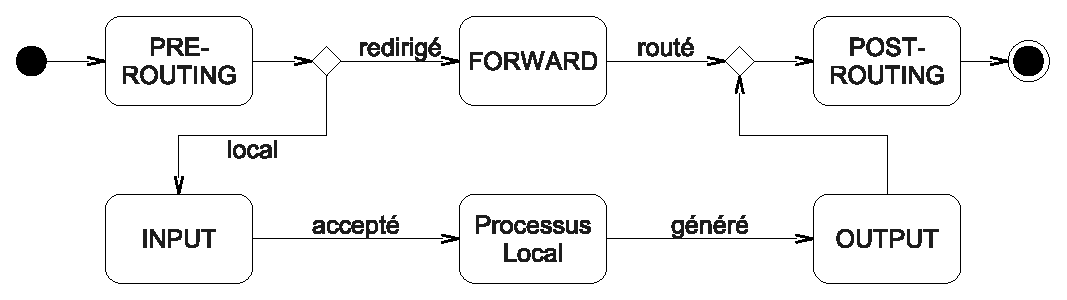
\includegraphics[width=\columnwidth]{firewall}
  \caption{Packet Filter Structure}
  \label{fig:netfilter}
\end{figure}

With the packet filter configuration, the individual chains of the 
packet filter can be modified directly. An individual array exists
for each chain, one for the
\fwchain{INPUT}-chain (\var{PF\_INPUT\_\%}), one for the
\fwchain{FORWARD}-chain (\var{PF\_FORWARD\_\%}), one for the
\fwchain{OUTPUT}-chain (\var{PF\_OUTPUT\_\%}), one for the
\fwchain{PREROUTING}-chain (managing port forwarding)
(\var{PF\_PREROUTING\_\%}), and one for the \fwchain{POSTROUTING}-chain,
managing packet masquerading (\var{PF\_POSTROUTING\_\%}).

An entry in one of these arrays consists mainly of an action (see below)
which can be restricted by additional conditions. These conditions
relate to properties of the considered packet. A packet contains
information about its origin (source PC that has sent the packet), 
its target (to which PC and which application should the packet be delivered)
and much more. Conditions can refer to the following properties of
a packet:

\begin{itemize}
  \item source (source address, source port or both)
  \item destination (destination address, destination port or both)
  \item protocol
  \item interface on which the packet comes in or goes out
  \item MAC-address of the originating PC
  \item state of the packet or the connection the packet comes from
\end{itemize}

If a packet comes in, the entries resp. the resulting rules generated
are processed from top to bottom and the first action to which all conditions
apply is performed. If none of the rules matches, the default action is executed,
which may be specified for (almost) any table.

An entry has the following format, bearing in mind that
all restrictions are optional:

\begin{example}
\begin{verbatim}
    restriction{0,} [[source] [destination]] action [BIDIRECTIONAL|LOG|NOLOG]
\end{verbatim}
\end{example}


At all points where networks, IP addresses or hosts need to be specified,
you can also refer to \var{IP\_NET\_\%}, \var{IP\_NET\_\%\_IPADDR} or
via \host{@hostname} to a host from \var{HOST\_\%}. If \var{OPT\_DNS}
is enabled, then outside of actions via \host{@fqdn} also hosts which
are \emph{nicht} mentioned in \var{HOST\_\%} can be referenced by their
names. This is particularly useful if dealing with external hosts which
also possess many (and changing) IP addresses.

\marklabel{sec:fwrules_actions}{\subsection{Packet Filter Actions}}

The following actions appy:
\begin{center}
    \begin{longtable}{|l|l|p{0.5\textwidth}|}
        \hline
        \multicolumn{1}{|l}{\textbf{Action}} &
        \multicolumn{1}{|l}{\textbf{chain(s)}} &
        \multicolumn{1}{|l|}{\textbf{Meaning}} \\
        \hline
        \endhead
        \hline
        \endfoot
        \endlastfoot
        \fwaction{ACCEPT}       & all
                                & Accept the packet.
                                \\
        \hline
        \fwaction{DROP}         &
                                \begin{tabular}[t]{@{}l@{}}
                                    \fwchain{INPUT} \\
                                    \fwchain{FORWARD} \\
                                    \fwchain{OUTPUT}
                                \end{tabular}
                                & Drop the packet (the sender recognizes that
                                just because no answer and no error message 
                                comes back).
                                \\
        \hline
        \fwaction{REJECT}       &
                                \begin{tabular}[t]{@{}l@{}}
                                    \fwchain{INPUT} \\
                                    \fwchain{FORWARD} \\
                                    \fwchain{OUTPUT}
                                \end{tabular}
                                & Reject the packet (the sender gets
                                a corresponding error message).
                                \\
        \hline
        \fwaction{LOG}          & all
                                & Log the packet and proceed to the next rule.
                                To distinguish log entries a prefix may be
                                used, specified by \fwaction{LOG:log-prefix}.
                                The maximum length of this prefix is 28
                                characters and it may contain letters, numbers,
                                hyphens (\texttt{-}), and underscores (\texttt{\_}).
                                \\
        \hline
        \fwaction{MASQUERADE}   & \fwchain{POSTROUTING}
                                & Mask the packet: Replace the source address
                                of the packet by the own one and make sure that
                                replies for this connection are redirected to 
                                the correct computer.
                                \\
        \hline
        \fwaction{SNAT}         & \fwchain{POSTROUTING}
                                & Replace source address and source port of the
                                packet by the address specified as a parameter
                                for \fwaction{SNAT} (for all packets belonging
                                to the connection in consideration).
                                \\
        \hline
        \fwaction{DNAT}         & \fwchain{PREROUTING}
                                & Replace destination address and destination port
                                of the packet by the address specified as a parameter
                                for \fwaction{SNAT} (for all packets belonging
                                to the connection in consideration).
                                \\
        \hline
        \fwaction{REDIRECT}     &
                                \begin{tabular}[t]{@{}l@{}}
                                    \fwchain{PREROUTING} \\
                                    \fwchain{OUTPUT}
                                \end{tabular}
                                & Replace destination port of the packet 
                                by the address specified as a parameter
                                for \fwaction{SNAT} (for all packets belonging
                                to the connection in consideration).
                                \\
        \hline
        \fwaction{NETMAP}       &
                                \begin{tabular}[t]{@{}l@{}}
                                    \fwchain{PREROUTING} \\
                                    \fwchain{POSTROUTING}
                                \end{tabular}
                                & Copy destination resp. source address of the
                                packet to the range specified as a parameter for
                                \fwaction{NETMAP}; the ports stay unchanged
                                (for all packets belonging to the connection 
                                in consideration; while changing the destination
                                address in the \fwchain{PREROUTING}-chain and the 
                                source address of the \fwchain{POSTROUTING}-chain).
                                \\
        \hline
        \caption{Packet Filter Actions}\marklabel{fwrule:actions}{}
    \end{longtable}
\end{center}

Some of these actions may be modified in behaviour by using the options 
\fwaction{BIDIRECTIONAL}, \fwaction{LOG} or \fwaction{NOLOG}.
\fwaction{BIDIRECTIONAL} generates the same rule a second time with
source and destination adresse exchanged (and source and destination
port exchanged and/or in- and outbound network interface exchanged if
specified). \fwaction{LOG}/\fwaction{NOLOG} activates resp. deactivates
logging for this rule.

\marklabel{sec:fwrules_limits}{\subsection{Restrictions For Rules}}

Restrictions may be defined by constraints explained in the following sections.
You may use \fwmatch{any} at any place where you don't want restrictions but
want/have to specify something. Constraints can be specified in any order
if they have a preceding prefix. This applies to all restrictions, except
for specifying a source or destination address which must always be placed
directly in front of the action, other constraints must be specified before.
Restrictions can also be negated, simply prefix them by a \fwmatch{!}.

\subsubsection{Constraints For Source And Target}

Each packet contains source and target informations in a tuple of an IP address and
ports.\footnote{A port only exists for TCP- and UDP-packets.} This source resp.
target can serve as a constraint and may be addressed like this:

\begin{center}
    \begin{longtable}{|l|p{0.5\textwidth}|}
        \hline
        \multicolumn{1}{|l}{\textbf{Expression}} &
        \multicolumn{1}{|l|}{\textbf{Meaning}} \\
        \hline
        \endhead
        \hline
        \endfoot
        \endlastfoot
    \verb+ip+               & a simple IP address\\
    \verb+network+          & a network declaration in the form of \verb+<ip>/<netmask>+ \\
    \verb+port[-port]+      & a port resp. a port range\\
    \verb+IP_NET_x_IPADDR+  & the IP address of the \verb+x+ router's interface\\
    \verb+IP_NET_x+         & the \verb+x+ router's subnet\\
    \verb+IP_ROUTE_x+       & the subnet \verb+x+ specified in the route
      (default routes can't be used, they would match \fwmatch{any} and are excluded precautiously)\\
    \verb+@name+            & one of the names or aliases set via HOST\_\%\_*; 
			      the associated IP address will be filled in here\\
    \verb+<ip oder netzwerk>:port[-port]+ & Host- resp. network address in one of the variants
			    above, combined with a port resp. port range\\
        \hline
        \caption{Constraints For Source And Target In Paket Filter Rules}
    \end{longtable}
\end{center}

\noindent Example: \verb+'192.168.6.2 any DROP'+

If two of these lines shine up the first will be considered as source
and the second as target. Hence, in this example we drop the packets
originating from the computer with the IP address 192.168.6.2, regardless
of where they are targeted.

If only one line exists the decision if target or source is meant will
be made depending on the value, which is quite easy:
\begin{itemize}
  \item If it contains a port value, target is meant,
  \item in all other cases the source is.
\end{itemize}

If you would like to shorten the example above you could write
\verb+'192.168.6.2 DROP'+. No port is mentioned, hence the constraint
is valid for the source (the machine the packet originated from).

If we were to allow communication with the \protocol{ssh}-deamon, we could
write \verb+'any any:22 ACCEPT'+ (packets from any machine to \protocol{ssh}-port
22 of any machine will be accepted) or even shorter \verb+'22 ACCEPT'+. Only
a port is mentioned, hence we address the target and thus all packets
targeted to port 22.

For simplification you may append \fwaction{BIDIRECTIONAL} to the action to
express that the rule is valid for both communication directions. Then rules
will be generated with source and target addresses and if applicable ports
and network interfaces exchanged while leaving the rest untouched.

Examples:
\medskip

\begin{example}
\noindent
{\footnotesize
 \begin{tabular}{@{}p{5cm}p{10cm}@{}}
    \verb+127.0.0.1 ACCEPT+             & local communication (source 127.0.0.1) is allowed\\
    \verb+any 192.168.12.1 DROP+        & packets to address 192.168.12.1 will be dropped\\
    \verb+any 192.168.12.1 DROP LOG+    & packets to address 192.168.12.1 will be dropped and logged additionally\\
    \verb+any 192.168.12.1 DROP NOLOG+  & packets to address 192.168.12.1 will be dropped but not logged\\
    \verb+22 ACCEPT+                    & packets to port 22 (\protocol{ssh}) will be accepted\\
    \verb+IP_NET_1_NET ACCEPT+          & packets from the subnet connected to the first interface will be accepted\\
    \verb+IP_NET_1_NET IP_NET_2_NET+    & communication between the subnets connected to the first and second\\
    \verb+  ACCEPT BIDIRECTIONAL+       & interface are allowed\\
 \end{tabular}
}
\end{example}

\subsubsection{Interface Constraints}

A rule can be restricted concerning the Interface on which a packet
was received resp. will be transmitted. The format is as follows:
\fwmatch{if:}\emph{in}\fwmatch{:}\emph{out}

In the \fwchain{INPUT}-chain the interface for outbound packets is not
restrictable (the packet does not leave anyway), in the \fwchain{POSTROUTING}-chain
the interface for received packets is not restrictable, because the
informations about it do not exist anymore. Only in the \fwchain{FORWARD}-chain
constraints for both can be defined.

Possible values for \emph{in} resp. \emph{out}:

\begin{itemize}
  \item \fwmatch{lo} (Loopback-interface, local communication on the router)
  \item \verb+IP_NET_x_DEV+
  \item \fwmatch{pppoe} (the PPPoE-interface; only with package \package{dsl}
		or \package{pppoe\_server} activated).
  \item \fwmatch{any}
\end{itemize}

\subsubsection{Protocol Constraints}

A rule can be restricted concerning the protocol a packet belongs to.
The format is as follows:
\fwmatch{prot:}\emph{protocol} resp. \fwmatch{prot:}\emph{icmp}\fwmatch{:}\emph{icmp-type}.
\emph{protocol} can be set to one of the following values:

\begin{itemize}
  \item \fwmatch{tcp}
  \item \fwmatch{udp}
  \item \fwmatch{gre} (Generic Routing Encapsulation)
  \item \fwmatch{icmp} (additionally you can specify a name for the ICMP-type to be filterd (\fwmatch{echo-reply} or
    \fwmatch{echo-request}), i.e. \fwmatch{prot:icmp:echo-request})
  \item numeric value of the protocol-ID (i.e. 41 for IPv6)
  \item \fwmatch{any}
\end{itemize}

If such a constraint does not exists, but port numbers should
be used in a rule, then the rule is generated \emph{twice},
once for the \protocol{tcp} and once for the \protocol{udp} protocol.

\subsubsection{MAC-Address Constraints}

Via \fwmatch{mac:}\emph{mac-address} constraints based on the MAC  address
may be specified.

\subsubsection{Packet State Constraints}

fli4l's packet filter gathers informations on the state of connections.
This informations can be used to filter packets, i.e let only packets pass that
belong to connections already existing. The state of a connection can take
this values:\footnote{see \altlink{http://www.sns.ias.edu/~jns/files/iptables_talk/x38.htm}
for a detailed description}

\begin{center}
    \begin{longtable}{|l|p{0.7\textwidth}|}
        \hline
        \multicolumn{1}{|l}{\textbf{State}} &
        \multicolumn{1}{|l|}{\textbf{Meaning}} \\
        \hline
        \endhead
        \hline
        \endfoot
        \endlastfoot
        \fwpktstate{INVALID}        & The packet does not belong to a know connection.
                                    \\
        \fwpktstate{ESTABLISHED}    & The packet belongs to a connection, where
                                    packets have already been transmitted in both
                                    directions.
                                    \\
        \fwpktstate{NEW}            & The packet has established a new connection
                                    or belongs to a connection that did not have
                                    packets transmitted in both directions.
                                    \\
        \fwpktstate{RELATED}        & The packet establishes a new connection,
                                    but has a relation to an already existing
                                    connection (i.e. \protocol{ftp} establishes
                                    a separate connection for data transfer).
                                    \\
        \hline
        \caption{Packet State Constraints in Packet Filter Rules}
    \end{longtable}
\end{center}

States are defined as follows:
\fwmatch{state:}\emph{state(s)}. If you want to specify more than one
state they have to be separated by commas. I.e. to let packets
pass that belong directly or indirectly to established connections
write \fwmatch{state:}\fwpktstate{ESTABLISHED,RELATED} (this makes
sense in \fwchain{INPUT}- or \fwchain{FORWARD}-chain).

\subsubsection{Constraints Based On The Frequency Of Actions}

Under certain circumstances you may wish to restrict the frequency of
actions, i.e. allow only one ICMP-Echo request per second. This may be
reached with \fwmatch{limit}-constraints, which look like this:
\fwmatch{limit:}\emph{Frequency:Burst}. The frequency is specified as
\emph{n/time units} (second, minute, hour, day), however, events may also occur
in rapid succession (Burst). \texttt{limit:3/minute:5} for example means
that a maximum of three events per minute is allowed, but also five events
in rapid succession will be accepted.

\marklabel{sec:templates}{\subsection{Using Templates With The Packet Filter}}

To simplify dealing with the packet filter you may summarize rules frequently
occuring in templates. Thus, it is possible to provide a wide range of
packet filtering rules and combine them in a collection with a symbolic
name. Instead of directly using protocols and port numbers, you may then
use entries such as \fwmatch{tmpl:ssh} if you want to use the \protocol{ssh}
protocol in a rule. How to deal with templates is shown here using the
example of \protocol{ssh}.

If you want to reach your fli4l from the Internet via \protocol{ssh},
write into an entry in the array variable \var{PF\_input\_\%} the
corresponding service name (here \protocol{ssh}) preceded by
\fwmatch{tmpl} and the action to apply for this service. Example:

\begin{example}
\begin{verbatim}
    PF_INPUT_2='tmpl:ssh ACCEPT'
\end{verbatim}
\end{example}

\fwmatch{tmpl:} means that the rule should be based on a template. Specify the
name of the service after the `:', adapted to our example hence \protocol{ssh}.
At last you have to set an action to be bound to the service. Since we want to
acces the fli4l over the internet, we allow the connection with \fwaction{ACCEPT}.
Restrictions for IP-addresses or nets are not provided so the \protocol{ssh}-service
will be accessible on all interfaces from all networks. If you want to invoke further
restrictions for accessing the \protocol{ssh}-service you may use the packet filter
notation already explained above.

For which services rules are predefined (e.g. templates exist) can be seen
in the template file at \verb+opt/etc/fwrules.tmpl/templates+. A list in a table
follows (see table \ref{tab:fwrules_tmpl}).

\begin{center}
  {\footnotesize
  \begin{longtable}{|lll|}
     \hline
     {\textbf{Template}} & {\textbf{Protocol}} & {\textbf{Port(s)}} \\
     \hline\hline
     \endhead
     \input{fwrules_tmpl_table.inc} \\
     \hline
     \caption{Templates Included With fli4l}
     \label{tab:fwrules_tmpl}
  \end{longtable}}
\end{center}

The Syntax for this kind of packet filter rules is

\begin{example}
\begin{verbatim}
    tmpl:<Name of the service> <Constraint> <Action>
\end{verbatim}
\end{example}

\verb+<Constraint>+ allows everything mentioned at \ref{sec:fwrules_limits}.
Possible values for \verb+<Action>+ are listed and described 
in \ref{sec:fwrules_actions}.

Some more examples should clarify the process. At first let's have a look at \var{PF\_PREROUTING}:

\begin{example}
\begin{verbatim}
    PF_PREROUTING_N='2'
    PF_PREROUTING_1='tmpl:xbl dynamic DNAT:@xbox'
    PF_PREROUTING_2='tmpl:https dynamic DNAT:192.168.193.250'
\end{verbatim}
\end{example}

The rule \var{PF\_PREROUTING\_1} supplies the Xbox with everything necessary
for Xbox Live. By the use of \fwmatch{tmpl:xbl} all ports and protocols used
for Xbox Live will be forwarded to the \host{xbox}. Instead of using an IP
address we use an entry from the \var{HOST\_\%\_NAME}-array. \fwmatch{dynamic}
tells the fli4l to forward all ports from the internet interface.

The second rule forwards the \protocol{https}-protocol to a webserver in a DMZ
(Demilitarized Zone).

No let's have a look at \var{PF\_INPUT}:

\begin{example}
\begin{verbatim}
    PF_INPUT_N='3'
    PF_INPUT_1='if:IP_NET_1_DEV:any ACCEPT'
    PF_INPUT_2='if:pppoe:any prot:tcp 113 ACCEPT'
    PF_INPUT_3='if:br0:any tmpl:dns @xbox IP_NET_1_IPADDR ACCEPT'
\end{verbatim}
\end{example}

The first rule allows access to the router for everyone from the net defined 
in \var{IP\_NET\_1}. The second rule opens the \protocol{ident}-port needed
for package \package{oident}. The third rule allows the xbox to access fli4l's
DNS server. Notice the use of a host alias here.

\var{PF\_FORWARD} and \var{PF\_POSTROUTING} do not provide
\fwmatch{tmpl}-specific content.

\begin{figure}[htbp]
  \centering
  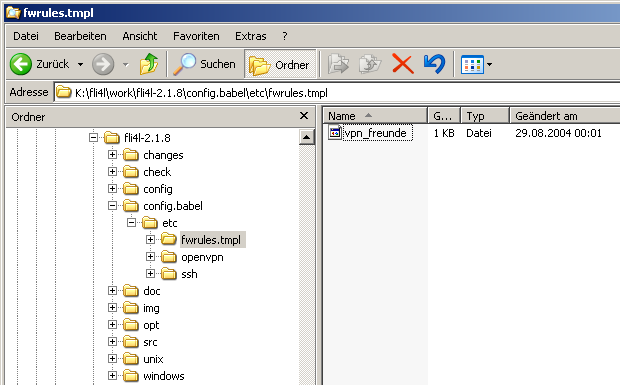
\includegraphics[width=0.9\columnwidth]{etc_fwrules_tmpl_dir}
  \caption{Directory Structure fli4l}
  \label{fig:etc_fwrules_tmpl_dir}
\end{figure}

It is also possible to create templates yourself or for other packages to
provide their own ones. To create a template you only need to create a text
file with the rules in it and name it like the template. For a private template
file use the directory \verb+etc/fwrules.tmpl+ (create it if necessary) under
your \texttt{config} directory as shown in picture \ref{fig:etc_fwrules_tmpl_dir}. 
Package developers or users needing templates for more than one configuration
may place their template files directly in \texttt{opt/etc/fwrules.tmpl}. 
The templates in the user's \texttt{config} directory override other settings, though.
The templates included in fli4l will be interpreted as the last ones. This enables you to
\glqq{}override\grqq{} fli4l's templates when providing templates by
the same name in your \texttt{config}-directory.

If, for example you like to create the template \fwmatch{vpn\_friends}, create a
file by the name \texttt{vpn\_friends}. The template should contain the services
\protocol{ssh}, \protocol{smtp}, \protocol{dns} and \protocol{samba}.
Hence you write the following to \texttt{vpn\_friends}:

\begin{example}
\begin{verbatim}
    prot:tcp 22
    prot:tcp 25
    53
    prot:udp 137-138
    prot:tcp 139
    prot:tcp 445
\end{verbatim}
\end{example}

\noindent Every time you use the template \fwmatch{vpn\_friends} rules will be
created for all contained protocols and ports.
\verb+PF_FORWARD_x='tmpl:vpn_friends ACCEPT'+ will create theses
\fwchain{FORWARD}-rules:

\begin{example}
\begin{verbatim}
    prot:tcp 22 ACCEPT
    prot:tcp 25 ACCEPT
    53 ACCEPT
    prot:udp 137-138 ACCEPT
    prot:tcp 139 ACCEPT
    prot:tcp 445 ACCEPT
\end{verbatim}
\end{example}

\subsection{Configuration Of The Packet Filter}

The packet filter is mainly configured by four array-variables:

\begin{itemize}
  \item \var{PF\_INPUT\_\%} configures the \fwchain{INPUT}-chain,
  \item \var{PF\_FORWARD\_\%} configures the \fwchain{FORWARD}-chain,
  \item \var{PF\_OUTPUT\_\%} configures the \fwchain{OUTPUT}-chain,
  \item \var{PF\_PREROUTING\_\%} configures the \fwchain{PREROUTING}-chain and
  \item \var{PF\_POSTROUTING\_\%} configures the \fwchain{POSTROUTING}-chain.
\end{itemize}

\configlabel{PF\_LOG\_LEVEL}{PFLOGLEVEL} For all chains following applies
the setting of the protocol level in \var{PF\_LOG\_LEVEL}, which may be
set to one of these values: \fwloglevel{debug}, \fwloglevel{info}, \fwloglevel{notice},
\fwloglevel{warning}, \fwloglevel{err}, \fwloglevel{crit}, \fwloglevel{alert},
\fwloglevel{emerg}.

\subsubsection{Then \fwchain{INPUT}-Chain}

The \fwchain{INPUT}-chain defines who is allowed to access the router.
If no rule of the \fwchain{INPUT}-chain matches, the default action
handles the packet and the protocol variable decides wheter a rejection
will be written to the system-protocol or not.

The following restrictions apply to the parameters:
\begin{itemize}
  \item Only \fwaction{ACCEPT}, \fwaction{DROP} and \fwaction{REJECT}
    can be specified as actions.
  \item If using interface constraints only the receiving
    interface can be restricted.
\end{itemize}

\begin{description}
\config{PF\_INPUT\_POLICY}{PF\_INPUT\_POLICY}{PFINPUTPOLICY}
This variable describes the default action to be taken if no other
rule applies. Possible values:

\begin{itemize}
\item \fwaction{ACCEPT} (not recommended)
\item \fwaction{REJECT}
\item \fwaction{DROP} (not recommended)
\end{itemize}

\config{PF\_INPUT\_ACCEPT\_DEF}{PF\_INPUT\_ACCEPT\_DEF}{PFINPUTACCEPTDEF}
If this variable is set to `yes' default rules will be generated needed for
the correct function of the router. Use `yes' as a default here.

If you want to configure the router's behaviour completely yourself you may
enter `no' here but you will have to define all rules on your own then.
An equivalent to the default behaviour would look like this (the explanation
of user defined chains can be found \jump{sec:userlists}{here}):

\begin{example}
{\footnotesize
\begin{verbatim}
    PF_INPUT_ACCEPT_DEF='no'
    #
    # limit ICMP echo requests - use a separate chain
    #
    PF_USR_CHAIN_N='1'
    PF_USR_CHAIN_1_NAME='usr-in-icmp'
    PF_USR_CHAIN_1_RULE_N='2'
    PF_USR_CHAIN_1_RULE_1='prot:icmp:echo-request length:0-150 limit:1/second:5 ACCEPT'
    PF_USR_CHAIN_1_RULE_2='state:RELATED ACCEPT'

    PF_INPUT_N='4'
    PF_INPUT_1='prot:icmp usr-in-icmp'
    PF_INPUT_2='state:ESTABLISHED,RELATED ACCEPT'
    PF_INPUT_3='if:lo:any ACCEPT'
    PF_INPUT_4='state:NEW 127.0.0.1 DROP BIDIRECTIONAL'
\end{verbatim}}
\end{example}

The first rule branches to the rate limited ``usr-in-icmp''-chain.
The second only accepts packets belonging to established connections
(packets that have either the state \fwpktstate{ESTABLISHED} or
\fwpktstate{RELATED}), and the third one allows local communication
(\verb+if:lo:any ACCEPT+). The fourth filters packets that pretend to
be local communication but are not accepted by the rules defined before.

If you work with OpenVPN, the rules have to be enhanced to enable packets used
by the chains there.

\begin{example}
\begin{verbatim}
    PF_INPUT_N='5'
    ...
    PF_INPUT_5='ovpn-chain'
\end{verbatim}
\end{example}

\config{PF\_INPUT\_LOG}{PF\_INPUT\_LOG}{PFINPUTLOG}
Defines if rejected packets should be logged by the kernel.
Log output can be directed to the syslog deamon by activating \var{OPT\_KLOGD}.

\config{PF\_INPUT\_LOG\_LIMIT}{PF\_INPUT\_LOG\_LIMIT}{PFINPUTLOGLIMIT}
Defines how often log entries will be generated. The frequency is described
as \emph{n/time units} with bursts in analog to the limit constraints, e.g.
\texttt{3/minute:5}. If this entry is empty a default of \texttt{1/second:5}
is used, if set to \texttt{none}, the limit constraints are disabled.

\configlabel{PF\_INPUT\_UDP\_REJ\_LIMIT}{PFINPUTUDPREJLIMIT}
\config{PF\_INPUT\_REJ\_LIMIT PF\_INPUT\_UDP\_REJ\_LIMIT}{PF\_INPUT\_REJ\_LIMIT}{PFINPUTREJLIMIT}
Specifies how often a \fwaction{REJECT}-packet is generated when rejecting
incoming packets. The frequency is described as \emph{n/time units} with bursts 
in analog to the limit constraints, e.g. \texttt{3/minute:5}. If this entry is
empty a default of \texttt{1/second:5} is used, if set to \texttt{none},
the limit constraints are disabled.

\config{PF\_INPUT\_ICMP\_ECHO\_REQ\_LIMIT}{PF\_INPUT\_ICMP\_ECHO\_REQ\_LIMIT}{PFINPUTICMPECHOREQLIMIT}
Defines how often fli4l should react to a ICMP-Echo-request.The frequency is
described as \emph{n/time units} with bursts in analog to the limit constraints,
e.g. \texttt{3/minute:5}. If the limit is reached packets will be ignored
(\fwaction{DROP}). If this entry is empty a default of \texttt{1/second:5}
is used, if set to \texttt{none}, the limit constraints are disabled.

\config{PF\_INPUT\_ICMP\_ECHO\_REQ\_SIZE}{PF\_INPUT\_ICMP\_ECHO\_REQ\_SIZE}{PFINPUTICMPECHOREQSIZE}
Defines the allowed size of an ICMP-Echo-request (in bytes). The packet header
has to be included in this setting besides the pure data. The default is 150 bytes.

\configlabel{PF\_INPUT\_x}{PFINPUTx}
\configlabel{PF\_INPUT\_x\_COMMENT}{PFINPUTxCOMMENT}
\config{PF\_INPUT\_N PF\_INPUT\_x PF\_INPUT\_x\_COMMENT}{PF\_INPUT\_N}{PFINPUTN}
A list of rules that describe which packets the router should accept resp. reject.
\end{description}

\subsubsection{The \fwchain{FORWARD}-Chain}

By using the \fwchain{FORWARD}-chain will be configured which packets are
forwarded by the router. If no rule of the \fwchain{FORWARD}-chain matches,
the default action handles the packet and the protocol variable decides
wheter a rejection will be written to the system-protocol or not.

With the used parameters the restriction applies that only the actions
\fwaction{ACCEPT}, \fwaction{DROP} and \fwaction{REJECT} are allowed.

\begin{description}
\config{PF\_FORWARD\_POLICY}{PF\_FORWARD\_POLICY}{PFFORWARDPOLICY}
This variable describes the default action to be taken if no other
rule applies. Possible values:

\begin{itemize}
\item \fwaction{ACCEPT}
\item \fwaction{REJECT}
\item \fwaction{DROP}
\end{itemize}

\config{PF\_FORWARD\_ACCEPT\_DEF}{PF\_FORWARD\_ACCEPT\_DEF}{PFFORWARDACCEPTDEF}
Determines if the router accepts packets belonging to established
connections. If this variable is set to `yes', fli4l generates
a rule for accepting packets of the according state automatically:

\verb+'state:ESTABLISHED,RELATED ACCEPT'+,

aswell as a rule to drop packets of unknown state:

\verb+'state:INVALID DROP'+.

and at last a rule to drop packets with faked IP addresses:

\verb+'state:NEW 127.0.0.1 DROP BIDIRECTIONAL'+.

In addition the other subsystems will generate some default rules~-- a
configuration without default rules with port forwarding and OpenVPN 
would contain at least the following rules:

\begin{example}
\begin{verbatim}
    PF_FORWARD_ACCEPT_DEF='no'
    PF_FORWARD_N='5'
    PF_FORWARD_1='state:ESTABLISHED,RELATED ACCEPT'
    PF_FORWARD_2='state:INVALID DROP'
    PF_FORWARD_3='state:NEW 127.0.0.1 DROP BIDIRECTIONAL'
    PF_FORWARD_4='pfwaccess-chain'
    PF_FORWARD_5='ovpn-chain'
\end{verbatim}
\end{example}

\config{PF\_FORWARD\_LOG}{PF\_FORWARD\_LOG}{PFFORWARDLOG}
Defines if rejected packets should be logged by the kernel.
Log output can be directed to the syslog deamon by activating \var{OPT\_KLOGD}.

\config{PF\_FORWARD\_LOG\_LIMIT}{PF\_FORWARD\_LOG\_LIMIT}{PFFORWARDLOGLIMIT}
Defines how often log entries will be generated. The frequency is described
as \emph{n/time units} with bursts in analog to the limit constraints, e.g.
\texttt{3/minute:5}. If this entry is empty a default of \texttt{1/second:5}
is used, if set to \texttt{none}, the limit constraints are disabled.

\configlabel{PF\_FORWARD\_UDP\_REJ\_LIMIT}{PFFORWARDUDPREJLIMIT}
\config{PF\_FORWARD\_REJ\_LIMIT PF\_FORWARD\_UDP\_REJ\_LIMIT}{PF\_FORWARD\_REJ\_LIMIT}{PFFORWARDREJLIMIT}
Specifies how often a \fwaction{REJECT}-packet is generated when rejecting
incoming packets. The frequency is described as \emph{n/time units} with bursts 
in analog to the limit constraints, e.g. \texttt{3/minute:5}. If this entry is
empty a default of \texttt{1/second:5} is used, if set to \texttt{none},
the limit constraints are disabled.

\configlabel{PF\_FORWARD\_x}{PFFORWARDx}
\configlabel{PF\_FORWARD\_x\_COMMENT}{PFFORWARDxCOMMENT}
\config{PF\_FORWARD\_N PF\_FORWARD\_x PF\_FORWARD\_x\_COMMENT}{PF\_FORWARD\_N}{PFFORWARDN}
A list of rules that describe which packets the router should forward resp. reject.

\end{description}

\subsubsection{The \fwchain{OUTPUT}-Chain}

The \fwchain{OUTPUT}-chain configures what the router is allowed to access. 
If no rule of the \fwchain{OUTPUT}-chain matches,
the default action handles the packet and the protocol variable decides
wheter a rejection will be written to the system-protocol or not.

With the used parameters the following restrictions apply:
\begin{itemize}
  \item Only \fwaction{ACCEPT}, \fwaction{DROP} and \fwaction{REJECT}
    can be specified as actions.
  \item For interface constraints only the output interface can
    be restricted.
\end{itemize}

\begin{description}
\config{PF\_OUTPUT\_POLICY}{PF\_OUTPUT\_POLICY}{PFOUTPUTPOLICY}
This variable describes the default action to be taken if no other
rule applies. Possible values:

\begin{itemize}
\item \fwaction{ACCEPT}
\item \fwaction{REJECT}
\item \fwaction{DROP}
\end{itemize}

\config{PF\_OUTPUT\_ACCEPT\_DEF}{PF\_OUTPUT\_ACCEPT\_DEF}{PFOUTPUTACCEPTDEF}
If this variable is set to `yes' default rules necessary for correct function of
the router will be generated. Use `yes' as a default here.

If you want to configure the router's behaviour completely yourself you may
enter `no' here but you will have to define all rules on your own then.
An equivalent to the default behaviour would look like this:

\begin{example}
{\footnotesize
\begin{verbatim}
    PF_OUTPUT_ACCEPT_DEF='no'

    PF_OUTPUT_N='1'
    PF_OUTPUT_1='state:ESTABLISHED,RELATED ACCEPT'
\end{verbatim}}
\end{example}

This single rule accepts only packets belonging to established connections
(e.g. packets of the state \fwpktstate{ESTABLISHED} or \fwpktstate{RELATED}).

\config{PF\_OUTPUT\_LOG}{PF\_OUTPUT\_LOG}{PFOUTPUTLOG}
Defines if rejected packets should be logged by the kernel.
Log output can be directed to the syslog deamon by activating \var{OPT\_KLOGD}.

\config{PF\_OUTPUT\_LOG\_LIMIT}{PF\_OUTPUT\_LOG\_LIMIT}{PFOUTPUTLOGLIMIT}
Defines how often log entries will be generated. The frequency is described
as \emph{n/time units} with bursts in analog to the limit constraints, e.g.
\texttt{3/minute:5}. If this entry is empty a default of \texttt{1/second:5}
is used, if set to \texttt{none}, the limit constraints are disabled.

\configlabel{PF\_OUTPUT\_UDP\_REJ\_LIMIT}{PFOUTPUTUDPREJLIMIT}
\config{PF\_OUTPUT\_REJ\_LIMIT PF\_OUTPUT\_UDP\_REJ\_LIMIT}{PF\_OUTPUT\_REJ\_LIMIT}{PFOUTPUTREJLIMIT}
Specifies how often a \fwaction{REJECT}-packet is generated when rejecting
incoming packets. The frequency is described as \emph{n/time units} with bursts 
in analog to the limit constraints, e.g. \texttt{3/minute:5}. If the limit is
exceeded packets will be ignored (\fwaction{DROP}). If this entry is
empty a default of \texttt{1/second:5} is used, if set to \texttt{none},
the limit constraints are disabled.

\configlabel{PF\_OUTPUT\_x}{PFOUTPUTx}
\configlabel{PF\_OUTPUT\_x\_COMMENT}{PFOUTPUTxCOMMENT}
\config{PF\_OUTPUT\_N PF\_OUTPUT\_x PF\_OUTPUT\_x\_COMMENT}{PF\_OUTPUT\_N}{PFOUTPUTN}
A list of rules that describe which packets the router should transmit resp. drop.
\end{description}

\marklabel{sec:userlists}{\subsubsection{User Defined Lists}}

In several cases you may want to establish own chains to filter packets
in detail there. These chains can be defined and filled with rules via 
\var{PF\_USR\_CHAIN\_\%}. The names of the chains have to start with 
\emph{usr-} and after their definition can be used everywhere in the 
\fwchain{INPUT}- or \fwchain{FORWARD}-chain as actions. The ICMP-filter 
chain used before will serve as an example here:

\begin{example}
{\footnotesize
\begin{verbatim}
    PF_USR_CHAIN_N='1'
    #
    # create usr-in-icmp
    #
    PF_USR_CHAIN_1_NAME='usr-in-icmp'
    #
    # add rule to usr-in-icmp
    #
    PF_USR_CHAIN_1_RULE_N='2'
    PF_USR_CHAIN_1_RULE_1='prot:icmp:echo-request length:0-150 limit:1/second:5 ACCEPT'
    PF_USR_CHAIN_1_RULE_2='state:RELATED ACCEPT'
    #
    # use chain in PF_INPUT
    #
    PF_INPUT_2='prot:icmp usr-in-icmp'
\end{verbatim}}
\end{example}

\begin{description}
\config{PF\_USR\_CHAIN\_N}{PF\_USR\_CHAIN\_N}{PFUSRCHAINN} Defines the number
of user defined chains.

\config{PF\_USR\_CHAIN\_x\_NAME}{PF\_USR\_CHAIN\_x\_NAME}{PFUSRCHAINxNAME}
Defines the name of an user defined chain. The name has to be prefixed by
\emph{usr-}.

\configlabel{PF\_USR\_CHAIN\_x\_RULE\_x}{PFUSRCHAINxRULEx}
\configlabel{PF\_USR\_CHAIN\_x\_RULE\_x\_COMMENT}{PFUSRCHAINxRULExCOMMENT}
\config{PF\_USR\_CHAIN\_x\_RULE\_N}{PF\_USR\_CHAIN\_x\_RULE\_N}{dummy0}
\config{PF\_USR\_CHAIN\_x\_RULE\_x}{PF\_USR\_CHAIN\_x\_RULE\_N}{dummy1}
\config{PF\_USR\_CHAIN\_x\_RULE\_x\_COMMENT}{PF\_USR\_CHAIN\_x\_RULE\_N}{PFUSRCHAINxRULEN}
These variables define the rules to be inserted in the user defined chain.
All rules may be used that are also valid for the \fwchain{FORWARD}-chain.
If no rule of the user defined chains matches, the router will return to
the parent chain and check the next rule after the branching to
the user defined rules.
\end{description}

\subsubsection{The NAT-Chains (Network Address Translation)}

Packets still can be changed after the routing decision. For example they
may get a new target address to be forwarded to another computer (port
forwarding) or a new source address may be inserted to mask the network
behind the router. Masquerading is used i.e. to provide internet access
for a private net over one public IP or a in DMZ-setup to hide the structure
of the local net from computers in the DMZ.\\

Configuration is done with two chains, \fwchain{PREROUTING}- and
\fwchain{POSTROUTING}-chain.\\
By the \fwchain{POSTROUTING}-chain the
packets are defined that have to be masked by the router. If no rule of
the \fwchain{POSTROUTING}-chain matches, the packets will be forwarded unmasked. 

Two variants exist for masquerading: one for network interfaces that do
get an IP address allocated on dialin (\fwaction{MASQUERADE}) and one for
network interfaces  with static IP address (\fwaction{SNAT}). \fwaction{SNAT}
in addition expects the source IP address to be inserted into the packet.
It may be specified as an:
\begin{itemize}
\item IP address (Example: \fwaction{SNAT:1.2.3.4}),
\item IP range (Example: \fwaction{SNAT:1.2.3.4-1.2.3.10})
\item or as symbolic reference (Example:
\fwaction{SNAT:IP\_NET\_1\_IPADDR})
\end{itemize}

For both \fwaction{SNAT} and \fwaction{MASQUERADE} a port or port range
may be set to which the source port may be redirected. Usually this notation is
necessary because the kernel can choose the ports on its own. But there exist
applications that desire the source port unchanged (and thus require 1:1-NAT) or
which forbid PAT (Port Address Translation) or NAPT (Network Address and Port
Translation). The port range is simply added to the end, like this:
\fwaction{SNAT:IP\_NET\_1\_IPADDR:4000-8000}.

With the \fwchain{POSTROUTING}-chain only \fwaction{ACCEPT}, \fwaction{SNAT},
\fwaction{NETMAP} and \fwaction{MASQUERADE} may be used as actions.

\begin{description}

\configlabel{PF\_POSTROUTING\_x}{PFPOSTROUTINGx}
\configlabel{PF\_POSTROUTING\_x\_COMMENT}{PFPOSTROUTINGxCOMMENT}
\config{PF\_POSTROUTING\_N PF\_POSTROUTING\_x PF\_POSTROUTING\_x\_COMMENT}{PF\_POSTROUTING\_N}{PFPOSTROUTINGN}
\mbox{}\newline
A list of rules that describe which packets the router should mask
resp. forward unmasked. If packets should be excluded from masking
an ACCEPT-rule for these packets may be put in front of the 
MASQUERADE rule.

\end{description}

The \fwchain{PREROUTING}-chain configures which packets should be transferred
to another computer. If no rule of the \fwchain{PREROUTING}-chain matches the
packets will be processed further without changes. The action \fwaction{DNAT} expects
the IP address to be inserted as the target address.
It may be specified as an:
\begin{itemize}
\item IP address (Example: \fwaction{DNAT:1.2.3.4}),
\item IP range (Example: \fwaction{DNAT:1.2.3.4-1.2.3.10})
\item or as a hostname (Example: \fwaction{DNAT:@client1})
\end{itemize}

At last a port or port range may be set to which the target port may be redirected. 
This is only necessary if the target port should be changed. The port (range) is
simply added to the end, like this:
\fwaction{DNAT:@server:21}.

\fwaction{REDIRECT} behaves like \fwaction{DNAT}, except for that the
Destination IP address is always set to the (primary) IP address of the interface on
which the packet came in so the packet is delivered locally. This
is needed i.e. for transparent proxies, see
\jump{OPTTRANSPROXY}{\var{OPT\_TRANSPROXY}}.

If you want a port forwarded to an interface with a dynamic address you do not know
to which IP the packet should be sent (at the time of configuration). Thus you can
use \fwmatch{dynamic} in the \fwchain{PREROUTING}-chain as a wildcard for the
IP address assigned later on, like this:

\begin{example}
{\footnotesize
\begin{verbatim}
    'dynamic:80  DNAT:1.2.3.4'           # forward http-packets to
                                         # IP address 1.2.3.4
    'prot:gre any dynamic DNAT:1.2.3.4'  # forward gre-packets (part of the  PPTP-
                                         # protocol) to IP address 1.2.3.4
\end{verbatim}}
\end{example}

Only \fwaction{ACCEPT}, \fwaction{DNAT}, \fwaction{NETMAP} and \fwaction{REDIRECT}
may be used as actions with the \fwchain{PREROUTING}-chain.

For further examples on port forwarding see the next paragraph.

\begin{description}

\configlabel{PF\_PREROUTING\_x}{PFPREROUTINGx}
\configlabel{PF\_PREROUTING\_x\_COMMENT}{PFPREROUTINGxCOMMENT}
\config{PF\_PREROUTING\_N PF\_PREROUTING\_x PF\_PREROUTING\_x\_COMMENT}{PF\_PREROUTING\_N}{PFPREROUTINGN}
\mbox{}\newline
A list of rules that describe which packets should be forwarded to another target by the router.

\end{description}

\subsection{Example}

Below see some examples of the packet filter configuration.

\subsubsection{The fli4l Default Configuration}

fli4l's default configuration for the
\fwchain{INPUT}-chain looks like this:

\begin{example}
\begin{verbatim}
    PF_INPUT_POLICY='REJECT'
    PF_INPUT_ACCEPT_DEF='yes'
    PF_INPUT_LOG='no'
    PF_INPUT_N='1'
    PF_INPUT_1='IP_NET_1 ACCEPT'
\end{verbatim}
\end{example}

By this we accomplish that
\begin{itemize}
\item computers in the local net are allowed to access the router\\
(\verb+PF_INPUT_1='IP_NET_1 ACCEPT'+),
\item local communication on the router itself is allowed
  (\verb+PF_INPUT_ACCEPT_DEF='yes'+),
\item packets belonging to connections established by the router are accepted
  \newline (\verb+PF_INPUT_ACCEPT_DEF='yes'+),
\item everything else is rejected (\verb+PF_INPUT_POLICY='REJECT'+),
\item but nothing is logged to the syslog
  (\verb+PF_INPUT_LOG='no'+).
\end{itemize}

The \fwchain{FORWARD}-chain looks alike: Only packets of our local
net and packets belonging to connections that were established by
machines in our local net should be forwarded. In addition NetBIOS-
and CIFS-packets will be dropped.

\begin{example}
\begin{verbatim}
    PF_FORWARD_POLICY='REJECT'
    PF_FORWARD_ACCEPT_DEF='yes'
    PF_FORWARD_LOG='no'
    PF_FORWARD_N='2'
    PF_FORWARD_1='tmpl:samba DROP'
    PF_FORWARD_2='IP_NET_1 ACCEPT'
\end{verbatim}
\end{example}

Note the dependance on the order of rules: \emph{At first} the
NetBIOS-packets are dropped and \emph{afterwards} the packets of
the local net are accepted.

The local net may communicate with the router, its packets get forwarded,
only the masking which is necessary for the internet access of a local
network is still missing:

\begin{example}
\begin{verbatim}
    PF_POSTROUTING_N='1'
    PF_POSTROUTING_1='IP_NET_1 MASQUERADE'
\end{verbatim}
\end{example}

\subsubsection{Trusted Nets}

If we do want to have several local subnets which should communicate with
each other free and unmasked we have to ensure that packets between those nets
don't get dropped or masked. In order to achieve this we add a rule or edit
the existing one.

Let's assume we have a DSL connection over PPPoE and the two subnets are
\var{IP\_NET\_1} (192.168.6.0/24) and \var{IP\_NET\_2} (192.168.7.0/24).
In this case the configuration would be as follows:

\begin{example}
\begin{verbatim}
    PF_FORWARD_POLICY='REJECT'
    PF_FORWARD_ACCEPT_DEF='yes'
    PF_FORWARD_LOG='no'
    PF_FORWARD_N='4'
    PF_FORWARD_1='IP_NET_1 IP_NET_2 ACCEPT BIDIRECTIONAL'
    PF_FORWARD_2='tmpl:samba DROP'
    PF_FORWARD_3='IP_NET_1 ACCEPT'
    PF_FORWARD_4='IP_NET_2 ACCEPT'

    PF_POSTROUTING_N='3'
    PF_POSTROUTING_1='IP_NET_1 IP_NET_2 ACCEPT BIDIRECTIONAL'
    PF_POSTROUTING_2='IP_NET_1 MASQUERADE'
    PF_POSTROUTING_3='IP_NET_2 MASQUERADE'
\end{verbatim}
\end{example}

The first rule ensures forwarding of packets between both subnets without further
processing. The third and fourth rule ensure that both subnets also have Internet
access. The first rule of the \fwchain{POSTROUTING}-chain provides unmasked
communication between both subnets.

In other words we could say that only packets transferred over the
\fwmatch{pppoe}-interface have to be masked:

\begin{example}
\begin{verbatim}
    PF_POSTROUTING_N='1'
    PF_POSTROUTING_1='if:any:pppoe MASQUERADE'
\end{verbatim}
\end{example}

We could as well have restricted the port filtering to the
\fwmatch{pppoe}-interface and combined both subnets to one,
as seen here:

\begin{example}
\begin{verbatim}
    PF_FORWARD_POLICY='REJECT'
    PF_FORWARD_ACCEPT_DEF='yes'
    PF_FORWARD_LOG='no'
    PF_FORWARD_N='2'
    PF_FORWARD_1='if:any:pppoe tmpl:samba DROP'
    PF_FORWARD_2='192.168.6.0/23 ACCEPT'

    PF_POSTROUTING_N='1'
    PF_POSTROUTING_1='if:any:pppoe MASQUERADE'
\end{verbatim}
\end{example}

Packets going out over the \fwmatch{pppoe}-interface and those addressed to 
\protocol{udp}-ports 137-138 or to \protocol{tcp}-ports 139 and 445 will be
dropped (rule~1), all other packets from subnet 192.168.6.0/23 will be 
forwarded (rule~2).

\subsubsection{Route Network}

Let's add a net 10.0.0.0/24 (i.e. a dial-in network) which we want to communicate
with unmasked, but packets to \protocol{udp}-ports 137-138 and to \protocol{tcp}-Ports
139 and 445 should be dropped:

\begin{example}
\begin{verbatim}
    PF_FORWARD_POLICY='REJECT'
    PF_FORWARD_ACCEPT_DEF='yes'
    PF_FORWARD_LOG='no'
    PF_FORWARD_N='4'
    PF_FORWARD_1='IP_NET_1 IP_NET_2 ACCEPT BIDIRECTIONAL'
    PF_FORWARD_2='tmpl:samba DROP'
    PF_FORWARD_3='192.168.6.0/23 ACCEPT'
    PF_FORWARD_4='10.0.0.0/24 ACCEPT'

    PF_POSTROUTING_N='2'
    PF_POSTROUTING_1='10.0.0.0/24 ACCEPT BIDIRECTIONAL'
    PF_POSTROUTING_2='192.168.6.0/23 MASQUERADE'
\end{verbatim}
\end{example}

\begin{itemize}
\item rule~1 allows unrestricted communication between the subnets
  \var{IP\_NET\_1} and \var{IP\_NET\_2}.
\item rule~2 drops packets to the samba ports.
\item rule 3 and 4 allow forwarding of packets orginating from the
  subnets 192.168.6.0/24, 192.168.7.0/24 and 10.0.0.0/24; the reverse
  direction is included by writing\\
  \verb+PF_FORWARD_ACCEPT_DEF='yes'+.
\item rule~1 of the \fwchain{POSTROUTING}-chain ensures that packets to
  resp. from the subnet 10.0.0.0/24-Subnetz are not masked.
\end{itemize}

An alternative:

\begin{example}
\begin{verbatim}
    PF_POSTROUTING_N='1'
    PF_POSTROUTING_1='if:any:pppoe MASQUERADE'
\end{verbatim}
\end{example}

This rule enables masking only for packets going out over the 
\fwmatch{pppoe}-interface.

\subsubsection{Blacklists, Whitelists}

Blacklists (a machine in this list is forbidden to do something) and
Whitelists (a machine in this list is allowed to do something) are
defined in a very similarl way. Rules are written that are very special at the beginning
and to the end are becoming more universal. With a blacklist rules are defined
that at the beginning forbid something and at the end allow something to
all not previously mentioned. With a Whitelist it is exactly the other way round.

\emph{Example~1:} All machines in subnet 192.168.6.0/24 except number 12
are allowed to access the Internet as long as they don't use CIFS Ports 137-138
(\protocol{udp}), 139 and 445 (\protocol{tcp}) to communicate:

\begin{example}
\begin{verbatim}
    PF_FORWARD_POLICY='REJECT'
    PF_FORWARD_ACCEPT_DEF='yes'
    PF_FORWARD_LOG='no'
    PF_FORWARD_N='3'
    PF_FORWARD_1='192.168.6.12 DROP'
    PF_FORWARD_2='tmpl:samba DROP'
    PF_FORWARD_3='192.168.6.0/23 ACCEPT'

    PF_POSTROUTING_N='1'
    PF_POSTROUTING_2='192.168.6.0/24 MASQUERADE'
\end{verbatim}
\end{example}

\emph{Example~2:} Only machine 12 has Internet access (with exception of the
ports mentioned above\ldots), all others are only allowed to communicate with
another local subnet:

\begin{example}
\begin{verbatim}
    PF_FORWARD_POLICY='REJECT'
    PF_FORWARD_ACCEPT_DEF='yes'
    PF_FORWARD_LOG='no'
    PF_FORWARD_N='3'
    PF_FORWARD_1='192.168.6.0/24 192.168.7.0/24 ACCEPT BIDIRECTIONAL'
    PF_FORWARD_2='tmpl:samba DROP'
    PF_FORWARD_3='192.168.6.12 ACCEPT'

    PF_POSTROUTING_N='1'
    PF_POSTROUTING_1='if:any:pppoe MASQUERADE'
\end{verbatim}
\end{example}

\subsection{Default Configurations}

\subsubsection{Simple Router Masking A Net Behind Itself}

\begin{example}
\begin{verbatim}
#
# Access to the router
#
PF_INPUT_POLICY='REJECT'
PF_INPUT_ACCEPT_DEF='yes'
PF_INPUT_LOG='no'
PF_INPUT_N='1'
PF_INPUT_1='IP_NET_1 ACCEPT'   # all hosts of the local net are allowed
                               # to access the router

#
# Internet access
#
PF_FORWARD_POLICY='REJECT'
PF_FORWARD_ACCEPT_DEF='yes'
PF_FORWARD_LOG='no'

PF_FORWARD_N='2'
PF_FORWARD_1='tmpl:samba DROP' # Samba-packets, that want to leave the
                               # net are dropped
PF_FORWARD_2='IP_NET_1 ACCEPT' # all other packets are allowed
                               # to leave the local net

#
# Maskieren des lokalen Netzes
#
PF_POSTROUTING_N='1'
PF_POSTROUTING_1='IP_NET_1 MASQUERADE'  # mask packets leaving the
                                        # subnet
\end{verbatim}
\end{example}

\subsubsection{Simple Router Masking Two Nets Behind Itself}

\begin{example}
\begin{verbatim}
#
# Access to the router
#
PF_INPUT_POLICY='REJECT'
PF_INPUT_ACCEPT_DEF='yes'
PF_INPUT_LOG='no'
PF_INPUT_N='2'
PF_INPUT_1='IP_NET_1 ACCEPT'   # all hosts of the local net are allowed
                               # to access the router
PF_INPUT_2='IP_NET_2 ACCEPT'   # all hosts of the local net are allowed
                               # to access the router

#
# Internet access
#
PF_FORWARD_POLICY='REJECT'
PF_FORWARD_ACCEPT_DEF='yes'
PF_FORWARD_LOG='no'

#
# Free communication between the nets
#
PF_FORWARD_N='4'
PF_FORWARD_1='IP_NET_1 IP_NET_2 ACCEPT BIDIRECTIONAL'
PF_FORWARD_2='tmpl:samba DROP' # Samba-packets, that want to leave the
                               # net are dropped
PF_FORWARD_3='IP_NET_1 ACCEPT' # all other packets are allowed
                               # to leave the local net
PF_FORWARD_4='IP_NET_2 ACCEPT' # all other packets are allowed
                               # to leave the local net

#
# Masking of local nets, unmasked communication between those nets
#
PF_POSTROUTING_N='3'
PF_POSTROUTING_1'IP_NET_1 IP_NET_2 ACCEPT BIDIRECTIONAL'
PF_POSTROUTING_2='IP_NET_1 MASQUERADE'  # mask packets leaving the
                                        # subnet
PF_POSTROUTING_3='IP_NET_2 MASQUERADE'  # mask packets leaving the
                                        # subnet
\end{verbatim}
\end{example}

\subsubsection{Masking DSL-Router With Two Nets Behind It And SSH/HTTP-Access From the Internet}

\begin{example}
\begin{verbatim}
#
# Access to the router
#
PF_INPUT_POLICY='REJECT'
PF_INPUT_ACCEPT_DEF='yes'
PF_INPUT_LOG='no'
PF_INPUT_N='4'
PF_INPUT_1='IP_NET_1 ACCEPT'   # all hosts of the local net are allowed
                               # to access the router
PF_INPUT_2='IP_NET_2 ACCEPT'   # all hosts of the local net are allowed
                               # to access the router
PF_INPUT_3='tmpl:ssh ACCEPT'   # allow access to the SSH service
                               # from everywhere
PF_INPUT_4='tmpl:http 1.2.3.4/24 ACCEPT'  # allow machines from
                               # a defined subnet access to the
                               # HTTP service


#
# Internet access
#
PF_FORWARD_POLICY='REJECT'
PF_FORWARD_ACCEPT_DEF='yes'
PF_FORWARD_LOG='no'

#
# No communication between the nets, both nets have
# Internet access, Samba-packets are dropped
#
PF_FORWARD_N='2'
PF_FORWARD_1='tmpl:samba if:any:pppoe DROP' # Samba-packets, that want to leave the
                               # net are dropped
PF_FORWARD_2='if:any:pppoe ACCEPT' # all other packets are allowed
                               # to leave the local net

#
# Masking of local nets, unmasked communication between those nets
#
PF_POSTROUTING_N='1'
PF_POSTROUTING_1='if:any:pppoe MASQUERADE'  # mask packets leaving the
                                            # subnet
\end{verbatim}
\end{example}

\subsubsection{Port Forwarding}

Port forwarding can be accomplished with the \fwchain{PREROUTING}-rules like
this (\verb+TARGET+ refers to the original target address (optional) and
the original target port, \verb+NEW_TARGET+ refers to the new target address
and new target port (optional), \verb+PROTOCOL+ refers to the protocol in use):

\begin{example}
\begin{verbatim}
    TARGET='<port>'
    NEW_TARGET='<ip>'
    PROTOCOL='<proto>'
    PF_PREROUTING_x='prot:<proto> dynamic:<port> DNAT:<ip>'

    TARGET='<port1>-<port2>'
    NEW_TARGET='<ip>'
    PROTOCOL='<proto>'
    PF_PREROUTING_x='prot:<proto> dynamic:<port1>-<port2> DNAT:<ip>'

    TARGET='<ip>:<port-a>'
    NEW_TARGET='<ip>:<port-b>'
    PROTOCOL='<proto>'
    PF_PREROUTING_x='prot:<proto> any <ip>:<port-a> DNAT:<ip>:<port-b>'
\end{verbatim}
\end{example}

\subsubsection{Transparent Proxy}
If access to the Internet should only be allowed over a local proxy
you may force this behaviour by the help of the \fwchain{PREROUTING}- and
\fwchain{POSTROUTING}-chains without the client noticing it.
In priciple you need to do this in three steps:

\begin{enumerate}
\item Redirect all HTTP-port-request to the Proxy except for its own ones
(\fwchain{PREROUTING}).
\item Change the redirected packets in a way that fools the proxy to think they
all come from the router so it will return its answers there
(\fwchain{POSTROUTING}).
\item Allow the packets to pass the FORWARD-chain, as far as an entry like

\begin{example}
\begin{verbatim}
PF_FORWARD_x='IP_NET_1 ACCEPT'
\end{verbatim}
\end{example}
does not exist (\fwchain{FORWARD}).
\end{enumerate}

\emph{Example~1:} Let's assume we only have one net \var{IP\_NET\_1},
a squid proxy is running there on a host by the name of \host{proxy} and
the whole \protocol{http}-traffic should be processed by it. Squid listens
on port 3128. For simplicity we refer via \host{@proxy} to the host
entered in \verb+HOST_1_NAME='proxy'+ (see
\jump{sec:domainkonfiguration}{Domain Configuration}).

Here are the resulting rules:

\begin{example}
\begin{verbatim}
...
  PF_PREROUTING_x='@proxy ACCEPT'
      # packets from the proxy should not be redirected

  PF_PREROUTING_x='prot:tcp IP_NET_1 80 DNAT:@proxy:3128'
      # HTTP-packets from IP_NET_1 will be redirected to @proxy, Port 3128
      # independet of the target

  PF_POSTROUTING_x='any @proxy:3128 SNAT:IP_NET_1_IPADDR'
      # change all packets to port 3128 in a way as if they came from
      # fli4l (IP_NET_1_IPADDR)

  PF_FORWARD_x='prot:tcp @proxy 80 ACCEPT'
      # let HTTP-packets from the proxy pass the FORWARD-chain (if necessary)
...
\end{verbatim}
\end{example}

If more nets or conflicting port forwardings (which are also \fwaction{DNAT}-rules)
exist, the rules may have to be more differentiated.

\emph{Example~2:} Our proxy by the name of \host{proxy} resides in \var{IP\_NET\_1},
listens to port 3128 and should only serve clients from \var{IP\_NET\_1}. 
\var{IP\_NET\_1} is reachabel over \var{IP\_NET\_1\_DEV}. Packets from other nets
should not be considered.

\begin{example}
\begin{verbatim}
...
  PF_PREROUTING_x='if:IP_NET_1_DEV:any !@proxy 80 DNAT:@proxy:3128'
      # Redirect queries to the HTTP-port that do not emerge from the proxy but
      # come in on an internal interface (IP_NET_1_DEV) to the proxy's port.
      # At this point it is important to check with if:IP_NET_1_DEV:any that the 
      # packets are coming from inside because otherwise packets from outside 
      # would also be redirected (security breakage)

  PF_POSTROUTING_x='prot:tcp IP_NET_1 @proxy:3128 SNAT:IP_NET_1_IPADDR'
      # Change HTTP-packets originating from IP_NET_1 and destinated to proxy-port 3128
      # in a way as if they came from fli4l (IP_NET_1_IPADDR)

  PF_FORWARD_x='prot:tcp @proxy 80 ACCEPT'
      # let HTTP-packets from the proxy pass the FORWARD-chain (if necessary)
...
\end{verbatim}
\end{example}

\emph{Example~3:} To ease our live and shorten the rules we may use
templates (see \jump{sec:templates}{Using Templates With The Packet Filter}).
At this point \fwmatch{tmpl:http}, translated in \fwmatch{prot:tcp any any:80}
is of advantage. \fwmatch{tmpl:http IP\_NET\_1 DNAT:@proxy:3128} then changes
to \fwmatch{prot:tcp IP\_NET\_1 80 DNAT:@proxy:3128}.

Both \var{IP\_NET\_1} and \var{IP\_NET\_2} should be redirected transparently
over the proxy. Simplified you could write:

\begin{example}
\begin{verbatim}
...
  PF_PREROUTING_x='tmpl:http @proxy   ACCEPT'
      # HTTP-packets from the proxy should not be redirected

  PF_PREROUTING_x='tmpl:http IP_NET_1 DNAT:@proxy:3128'
      # HTTP-packets from IP_NET_1 should be redirected

  PF_PREROUTING_x='tmpl:http IP_NET_2 DNAT:@proxy:3128'
      # HTTP-packets from IP_NET_2 should be redirected

  PF_POSTROUTING_x='IP_NET_1 @proxy:3128 SNAT:IP_NET_1_IPADDR'
  PF_POSTROUTING_x='IP_NET_2 @proxy:3128 SNAT:IP_NET_2_IPADDR'

  PF_FORWARD_x='tmpl:http @proxy ACCEPT'
...
\end{verbatim}
\end{example}

You may continue here forever\ldots

\marklabel{sec:dmz}{\subsection{DMZ~-- Demilitarized Zone}}

fli4l may also serve to build a DMZ. As this is only another additional
ruleset for the router please refer to the wiki at
https://ssl.nettworks.org/wiki for the time being.

\marklabel{sec:masqueradingmodule}{\subsection{Conntrack-Helpers}}

  Using IP-Masquerading\index{Masquerading} has the advantage
  that a bunch of machines in the LAN can be routed over only one
  official IP-address. However, there are also disadvantages that
  you have to take into account.

  A big problem for example is that no machine from outside can
  contact the machines in the LAN. This may be desired for security
  reasons but certain protocols will not work anymore because they
  require a connection from outside.

  A classic example is FTP. Beside a communication channel to exchange
  commands and answers another channel is needed (an IP-port) to
  transfer the actual data. fli4l uses certain conntrack-helpers for
  this in order to open such ports instantaneously and redirect them
  to the machine in question when needed. The conntrack-helper
  ``listens'' to the data stream to recognize when such an additional
  port is needed.

  Typical applications for conntrack-helpers are i.e. chat-protocols and
  Internet games.

  Conntrack-helper are activated over rules in two special arrays.
  The array \var{PF\_PREROUTING\_CT\_\%} contains helper-assignments
  to packets coming from outside, the array \var{PF\_OUTPUT\_CT\_\%}
  contains helper-assignments to packets generated on the router.
  Some practical examples help to illustrate this.
  
  \emph{Example 1:} If active FTP from the LAN should be allowed this is, 
  from the router's view, a connection from outside the router, thus an
  entry in \var{PF\_PREROUTING\_CT\_\%} has to be created:
  
\begin{example}
\begin{verbatim}
    PF_PREROUTING_CT_N='1'
    PF_PREROUTING_CT_1='tmpl:ftp IP_NET_1 HELPER:ftp'
\end{verbatim}
\end{example}

  The \protocol{ftp}-helper module will be loaded for all TCP connections from the
  local network (\var{IP\_NET\_1}) to any other addresses' port 21 (which is the
  \protocol{ftp}-Port). This module will allow the FTP server to establish a data
  transfer connection back to the client during this connection by opening a ``hole''
  in the firewall temporarily.

  \emph{Example 2:} If you want to enable passive ftp for a FTP server on the LAN
  (the data connection is established from the outside to the inside, so
  that a hole in the firewall must be opened here as well), this is also seen
  as a connection from outside by the router. Here we see the rule as for this:

\begin{example}
\begin{verbatim}
    PF_PREROUTING_CT_N='1'
    PF_PREROUTING_CT_1='tmpl:ftp any dynamic HELPER:ftp'
\end{verbatim}
\end{example}

  By this rule it is expressed that all FTP connections to the dynamic address
  of the router are associated to the FTP conntrack helper. Here \fwmatch{dynamic}
  was used because it is assumed that the router is responsible for dialing in to
  the Internet and thus has an external IP address. If the router performs dial-in
  via DSL, the rule can also be written as:

\begin{example}
\begin{verbatim}
    PF_PREROUTING_CT_N='1'
    PF_PREROUTING_CT_1='tmpl:ftp if:pppoe:any HELPER:ftp'
\end{verbatim}
\end{example}

  By this rule it is expressed that all FTP connections coming from the DSL
  interface (\fwmatch{pppoe}) are associated to the conntrack helper.

  If the router is not dialing, but e.g. is behind another router (Fritz! box,
  cable modem, a.s.o.) the following rules can be used:

\begin{example}
\begin{verbatim}
    PF_PREROUTING_CT_N='1'
    PF_PREROUTING_CT_1='tmpl:ftp if:IP_NET_2_DEV:any HELPER:ftp'
\end{verbatim}
\end{example}

  It is assumed in the Example, that the connection to the other router
  is performed over the interface associated with the second subnet
  (\var{IP\_NET\_2\_DEV}).

  Remember that of course an \emph{additional} configuration of the
  \fwchain{FORWARD}-chain is needed to really forward the FTP-packets. 
  A typical rule would be
  
\begin{example}
\begin{verbatim}
    PF_PREROUTING_1='tmpl:ftp any dynamic DNAT:@ftpserver'
\end{verbatim}
\end{example}

  assuming that the host running the FTP-server has the name \host{ftpserver}.

  \emph{Example 3:} If you like to use active FTP directly from fli4l (perhaps with 
  the help of the \protocol{ftp} program from the \package{Tools}-package) the firewall
  has to be prepared, this time in the \fwchain{OUTPUT}-chain by using 
  the array \var{PF\_output\_CT\_\%}:

\begin{example}
\begin{verbatim}
    PF_OUTPUT_CT_N='1'
    PF_OUTPUT_CT_1='tmpl:ftp HELPER:ftp'
\end{verbatim}
\end{example}

  This rule is not necessary if \verb+FTP_PF_ENABLE_ACTIVE='yes'+
  is used -- see the documentation for the \protocol{ftp}-OPT in
  the \package{tools}-package.

  Following is an overview over the existing conntrack-helpers:

\begin{center}
    \begin{longtable}{|l|p{0.5\textwidth}|}
        \hline
        \multicolumn{1}{|l}{\textbf{Helper}} &
        \multicolumn{1}{|l|}{\textbf{Explanation}} \\
        \hline
        \endhead
        \hline
        \endfoot
        \endlastfoot
            \index{ftp}\protocol{ftp}      & File Transfer Protocol\\
        \hline
            \index{h323}\protocol{h323}    & H.323 (Voice over IP)\\
        \hline
            \index{irc}\protocol{irc}      & Internet Relay Chat\\
        \hline
            \index{pptp}\protocol{pptp}    & PPTP Masquerading
                (By the use of this module it is possible to run more than one PPTP-Client
                behind the fli4l router at the same time.)\\
        \hline
            \index{sip}\protocol{sip}      & Session Initiation Protocol \\
        \hline
            \index{sane}\protocol{sane}    & SANE Network Procotol \\
        \hline
            \index{snmp}\protocol{snmp}    & Simple Network Management Protocol \\
        \hline
            \index{tftp}\protocol{tftp}    & Trivial File Transfer Protocol \\
        \hline
        \caption{Available Conntrack Helpers In The Packet Filter}\marklabel{fwrule:cthelpers}{}
    \end{longtable}
\end{center}

  Here is an overview over the variables to configure:

\begin{description}

\config{PF\_PREROUTING\_CT\_ACCEPT\_DEF}{PF\_PREROUTING\_CT\_ACCEPT\_DEF}{PFPREROUTINGCTACCEPTDEF}
If this variable is set to `yes', default rules are generated that
are necessary for proper functioning of the router. By default, you should use `yes' here.

\configlabel{PF\_PREROUTING\_CT\_x}{PFPREROUTINGCTx}
\configlabel{PF\_PREROUTING\_CT\_x\_COMMENT}{PFPREROUTINGCTxCOMMENT}
\config{PF\_PREROUTING\_CT\_N PF\_PREROUTING\_CT\_x PF\_PREROUTING\_CT\_x\_COMMENT}{PF\_PREROUTING\_CT\_N}{PFPREROUTINGCTN}
List of rules that describe which incoming packets are associated with
conntrack helpers by the router.

\config{PF\_OUTPUT\_CT\_ACCEPT\_DEF}{PF\_OUTPUT\_CT\_ACCEPT\_DEF}{PFOUTPUTCTACCEPTDEF}
If this variable is set to `yes', default rules are generated that
are necessary for proper functioning of the router. By default, you should use `yes' here.

\configlabel{PF\_OUTPUT\_CT\_x}{PFOUTPUTCTx}
\configlabel{PF\_OUTPUT\_CT\_x\_COMMENT}{PFOUTPUTCTxCOMMENT}
\config{PF\_OUTPUT\_CT\_N PF\_OUTPUT\_CT\_x PF\_OUTPUT\_CT\_x\_COMMENT}{PF\_OUTPUT\_CT\_N}{PFOUTPUTCTN}
\mbox{}\\
List of rules that describe which packets generated on the router are associated with
conntrack helpers by the router.

\end{description}

% Do not remove the next line
% Synchronized to r40999

\marklabel{sec:domainkonfiguration}{\section{Configuration du domaine}}

  Dans un LAN les ordinateurs Windows ont des caractéristiques désagréables~:
  si vous avez besoin d'utiliser un serveur de nom (ou DNS), vous devez
  configurer vos PC Windows pour ce service. Le problème c'est que les PCs
  Windows questionnent à intervalle régulier le serveur~-- même si personne
  n'utilise l'ordinateur~!
  Si vous configurez un serveur-DNS sur Internet pour votre PC Windows, cela
  pourrait revenir très cher \ldots

  Le truc est le suivant~: s'il n'y a pas de serveur DNS disponible sur
  le LAN (ou réseau local), on peut utiliser le routeur fli4l comme
  serveur DNS.

  DNSMASQ est utilisé en tant que serveurs DNS.

  Avant que nous commençions la configuration du DNS, vous devez d'abord
  réfléchir au nom de domaine et aux noms des PCs avant de les écrire dans
  votre réseau local. Le nom de domaine que vous emploierez ne sera pas
  visible sur Internet. Ainsi vous êtes libre pour employer presque
  n'importe quel nom de domaine.

  Vous devez donner un nom à chaque ordinateur de Windows dans votre réseau.
  En outre le routeur-fli4l doit avoir connaissance de ces noms.

  \begin{description}
    \config{DOMAIN\_NAME}{DOMAIN\_NAME}{DOMAINNAME}

    Configuration par défaut~: \var{DOMAIN\_NAME='lan.fli4l'}

      {Dans la version fli4l le nom de domaine "lan.fli4l" est paramètrè par 
      défaut. Vous êtes libre d'écrire votre propre nom de domaine. Vous devez
      éviter d'utiliser un nom qui pourrait exister sur Internet.
      Si vous employez un nom de domaine existant (par ex. france3.fr), vous ne
      pourrez pas accéder à ce domaine.}

    \config{DNS\_FORWARDERS}{DNS\_FORWARDERS}{DNSFORWARDERS}

    Configuration par défaut~: \var{DNS\_FORWARDERS=''}

      {On indique dans cette variable l'adresse IP du serveur DNS de votre
      Fournisseur Accès Internet (ou FAI), si fli4l est utilisé comme routeur
      pour Internet. Le routeur fli4l expédie à cette adresse toutes les
      requêtes DNS auxquelles il ne peut pas répondre.

      Vous pouvez entrer plusieurs adresses IP pour les serveurs DNS, vous devez
      séparer toutes les adresses IP par un espace (ou un blanc).

      Si plusieurs serveurs DNS sont configurés, les requêtes DNS seront utilisés
	  dans l'ordre de configuration des serveurs, ainsi le deuxième serveur spécifié
	  sera utilisé seulement si le premier n'a pas répondu à la requête DNS, etc.

      Il est également possible d'ajouter en option un numéro de port à
      l'adresse IP, pour cela, il faut séparer l'adresse IP et le port par deux
      points. Toutefois, il est nécessère d'activer la variable
      \jump{OPTDNS}{\var{OPT\_DNS='yes'}} dans le (paquetage
      \jump{sec:dnsdhcp}{dns\_dhcp}), cependant, cette variable
      ne doit jamais être substituée à la variable \var{*\_USEPEERDNS}.

      Attention~:
        \begin{itemize}
        \item \jump{PPPOEUSEPEERDNS}{\var{PPPOE\_USEPEERDNS}},
        \item \jump{ISDNCIRCxUSEPEERDNS}{\var{ISDN\_CIRC\_x\_USEPEERDNS}}
        ou
        \item \jump{DHCPCLIENTxUSEPEERDNS}{\var{DHCPCLIENT\_x\_USEPEERDNS}}
        \end{itemize}

        L'une de ces variables doit être paramétrées sur (='yes'), cela est
        nécessaire pour que le serveur DNS externe soit enregistré, sinon après
        le démarrage du routeur aucune résolution de nom ne sera possible.
        Le serveur DNS externe ne fonctionnera pas.

      Exception~: si vous configurez le routeur fli4l dans un réseau local 
      \emph{sans} connexion Internet ou dans un réseau avec un serveur DNS
      supplémentaire (réseau d'entreprise). Dans ce cas vous devez paramètrer
      l'adresse IP 127.0.0.1 pour empêcher le forwarding (empêcher les connexions
      extérieure).}

    \config{HOSTNAME\_IP}{HOSTNAME\_IP}{HOSTNAMEIP} (optionnelle)

    {Avec cette variable optionnelle vous pouvez définir, le réseau 'IP\_NET\_x'
    qui sera rattaché au \var{HOSTNAME} (ou nom d'Hôte).}

    \config{HOSTNAME\_ALIAS\_N}{HOSTNAME\_ALIAS\_N}{HOSTNAMEALIASN} (optionnelle)

    {Dans cette variable vous indiquez, le nombre d'alias (ou de surnom)
    supplémentaire pour le routeur.}

    \config{HOSTNAME\_ALIAS\_x}{HOSTNAME\_ALIAS\_x}{HOSTNAMEALIASx} (optionnelle)

    {Dans cette variable vous indiquez, l'alias pour le routeur.}

  \end{description}

% Synchronized to r29848

  \section{imond configuration}

  \begin{description}

    \config{OPT\_IMOND}{OPT\_IMOND}{OPTIMOND}

      Default setting: \var{OPT\_\-IMOND='no'}
    
    {\var{OPT\_\-IMOND} controls whether to start the imond server or not.
      The imond server is responsible for monitoring/controlling the fli4l
      router and for the so-called least cost routing. You can
      find a detailed description of the
      \jump{IMONDSCHNITTSTELLE}{Client/Server interface imond} in a separate
      appendix.

      Important: The least cost routing funtionality of fli4l can only be used
      when imond is running. Time-based switching of connections is impossible
      without imond!

      Starting with version 1.5, imond is mandatory for ISDN and DSL routing.
      In this case you have to set \var{OPT\_\-IMOND}='yes'. If you use fli4l
      as a router between LANs only, you should set \var{OPT\_\-IMOND}='no'.}

    \config{IMOND\_PORT}{IMOND\_PORT}{IMONDPORT}

    {The TCP/IP port where imond should wait for connections. You shouldn't
      change the default value `5000' unless in very exceptional cases.}


    \config{IMOND\_PASS}{IMOND\_PASS}{IMONDPASS}

      Default setting: \var{IMOND\_\-PASS=''}

    {This variable can be used to set a user password for imond.
      If a client connects to imond at port 5000, imond expects the client to
      provide this password before processing any requests, with the exception
      of the commands ``quit'', ``help'', and ``pass''. If you leave
      \var{IMOND\_\-PASS} empty, no password is necessary.

      The variables
      \begin{itemize}
      \item \jump{IMONDENABLE}{IMOND\_ENABLE},
      \item \jump{IMONDDIAL}{IMOND\_DIAL},
      \item \jump{IMONDROUTE}{IMOND\_ROUTE}, and
      \item \jump{IMONDREBOOT}{IMOND\_REBOOT}
      \end{itemize}
      control whether providing the user password is sufficient to execute the
      control commands like Dial, Hangup, Reboot, or Changing the Default Route, or
      whether you need a special admin password for these requests (see below).}

    \config{IMOND\_ADMIN\_PASS}{IMOND\_ADMIN\_PASS}{IMONDADMINPASS}

    Default setting: \var{IMOND\_ADMIN\_\-PASS=''}

    {Using the Admin Passwords the client receives all the rights and
    can thus use all control functions of the server imond~-- regardless 
    of the content of the variables \var{IMOND\_\-ENABLE}, \var{IMOND\_\-DIAL} etc.
    If you leave \var{IMOND\_\-ADMIN\_\-PASS} empty, the user password is
    sufficient to gain all rights!
    }

    \config{IMOND\_LED}{IMOND\_LED}{IMONDLED}

    {The imond server is able to display the router's online/offline state via
     a LED. This LED is connected to a serial port as follows:

      25 pin connector:

\begin{example}
\begin{verbatim}
        20 DTR  -------- 1kOhm ----- >| ---------- 7 GND
\end{verbatim}
\end{example}


      9 pin connector:
\begin{example}
\begin{verbatim}
         4 DTR  -------- 1kOhm ----- >| ---------- 5 GND
\end{verbatim}
\end{example}

      The LED is on if an ISDN or DSL connection is established, otherwise
      it is off. If you want this the other way round you have to reverse the polarity of
      the LED. You can reduce the dropper resistor down to 470 ohm if the LED
      is lit too dimly.

      It is also possible to use two different coloured LEDs. In this
      case you have to connect the second LED together with a dropper
      resistor between DTR and GND too, but with reversed polarity. Then either the
      first or the second LED will be lit depending on the router's state.
      Another possibility is to use a DUO LED (two-coloured, three pins).

      Currently, the serial port's RTS pin behaves exactly as the DTR pin.
      You could even attach a third LED for displaying the
      online/offline state. However, this behaviour may change in the future.

      The variable \var{IMOND\_\-LED} has to be set to the name of the serial
      port to where the LED is attached; possible values are `com1', `com2',
      `com3', and `com4'. Leave the variable empty if you don't use an LED.}


    \config{IMOND\_BEEP}{IMOND\_BEEP}{IMONDBEEP}

    {If setting \var{IMOND\_\-BEEP}='yes', imond will emit a two-tone sound
      over the PC speaker whenever the router's state changes from offline to
      online and the other way round. In the first case, the higher tone
      follows the lower one. In the second case, the higher tone is emitted
      before the lower one.}


    \config{IMOND\_LOG}{IMOND\_LOG}{IMONDLOG}

     Default setting: \var{IMOND\_\-LOG='no'}
    
    {You can set \var{IMOND\_LOG}='yes' in order to log connections in the
      file \verb+/var/log/imond.log+. This file can be copied i.e. by scp to
      another host e.g. for statistical purposes. However, using scp requires
      you to install and configure the sshd package appropriately.

      The structure of the log file entries is described in Table \ref{tab:imondlog}.
      \begin{table}[htbp]
        \small
        \centering
        \caption{Structure of Imond log files}\label{tab:imondlog}
        \begin{tabular}{lp{12cm}}
          \hline
          Entry & Meaning \\
          \hline
          Circuit & the name of the circuit for which the entry has been created \\
          Start time & the date and time of dialing this circuit \\
          Stop time & the date and time of hanging up this circuit \\
          Online time & the time this circuit was online \\
          Billed time & the time for which the provider will charge you (depends on
          the timing) \\
          Costs & the costs the provider will charge to your account \\
          Bandwidth & the bandwidth used, separated into ``in'' and ``out''
          (``in'' coming first), presented as two unsigned integer numbers
          for which the following applies: Bandwidth =\newline
          \emph{4GiB~$*<$first~number$>+<$second~number$>$} \\
          Device & the device used for communication \\
          Invoice pulse & the invoice pulse used by the provider for charging
          (taken from the circuit configuration)\\
          Call charge & the fee charged per invoice pulse (taken from the
          circuit configuration)\\
          \hline
        \end{tabular}
      \end{table}

      The costs are denoted in Euro. These values are only meaningful if you
      correctly define the corresponding circuit variables
      \jump{ISDNCIRCxTIMES}{\var{ISDN\_CIRC\_x\_TIMES}}}.

    \config{IMOND\_LOGDIR}{IMOND\_LOGDIR}{IMONDLOGDIR}

    {If the imond log is activated, this variable can be used to choose an
    alternative log directory instead of the default /var/log, e.g. /boot.
    This is useful in order to make the log persistent on the boot medium.
    However, this requires the boot medium to be mounted read/write.

    The default value is 'auto' which lets the fli4l router to determine the
    storage location automatically. Depending on further configuration, the
    storage path is /boot/persistent/base or some other path determined by
    the FLI4L\_UUID variable. If neither FLI4L\_UUID is set nor /boot is mounted
    read/write, the log file can be found under /var/run.}

    \configlabel{IMOND\_DIAL}{IMONDDIAL}
    \configlabel{IMOND\_ROUTE}{IMONDROUTE}
    \configlabel{IMOND\_REBOOT}{IMONDREBOOT}
    \config{IMOND\_ENABLE  IMOND\_DIAL  IMOND\_ROUTE  IMOND\_REBOOT}{IMOND\_ENABLE}{IMONDENABLE}

    {These variables make certain imond commands available in user mode
    (enabling/disabling the ISDN interface, dialing/hanging up, changing the
    default route, rebooting the router).

    Default settings:

\begin{example}
\begin{verbatim}
        IMOND_ENABLE='yes'
        IMOND_DIAL='yes'
        IMOND_ROUTE='yes'
        IMOND_REBOOT='yes'
\end{verbatim}
\end{example}

      All other features of imond's Client-Server interface are described in a
      \jump{IMONDSCHNITTSTELLE}{separate chapter}.}

  \end{description}

% Do not remove the next line
% Synchronized to r29829

  \section{Configuration du circuit général}

  \begin{description}
    \config{IP\_DYN\_ADDR}{IP\_DYN\_ADDR}{IPDYNADDR}

    {Si une connexion avec une IP dynamique est utilisée, vous
     devez placée la variable \var{IP\_\-DYN\_\-ADDR} sur 'yes', ou
     sur 'no' si statique. La plupart des fournisseurs d'accés utilisent
     une IP dynamique.

      Configuration par défaut~: \var{IP\_\-DYN\_\-ADDR}='yes'}

    \config{DIALMODE}{DIALMODE}{DIALMODE}

    {Par défaut fli4l utilise 'auto' pour le mode de numérotation,
     c-à-d. une connexion sera établie automatiquement dès qu'un ordinateur
     du réseau local essayera d'accéder à une adresse IP extérieure par ex.
     Internet. Il est également possible de spécifier le modes de connexion
     'manual' ou 'off'. Dans ce cas, la connexion peut uniquement être déclenchée
     en utilisant le client imonc.

      Configuration par défaut~: \var{DIALMODE}='auto'}

  \end{description}

% Do not remove the next line
% Synchronized to r38958

  \chapter{Les paquetages}

  En plus de l'installation de la base (BASE) il existe d'autres paquetages. Il
  s'agit notamment de "OPTs"\footnote{abréviation pour "module OPTionnel"}
  supplémentaire, qui peuvent au besoin être installés dans la base. Certains
  de ces OPTs sont intégrés dans le paquetage base, les autres sont à télécharger
  part. Une vue d'ensemble les paquetages fournis par l'équipe fli4l peuvent
  être téléchargés sur cette page Web
  (\altlink{http://www.fli4l.de/fr/telechargement/version-stable/}). D'autres
  paquetages crées par des concepteurs privés peuvent être trouvés dans la banque
  de données OPT (\altlink{http://extern.fli4l.de/fli4l_opt-db3/}). Nous allons
  voir dans les paragraphes suivant une description des paquetages créés et
  utilisés par l'équipe fli4l.


  \section{Outils dans le paquetage base}

  Dans le paquetage base vous trouverez les OPTs suivants~:

  \begin{center}
  \begin{tabular}{@{}lp{12cm}@{}}\hline
    Nom                & Description \\\hline
    \var{OPT\_SYSLOGD} & \jump{OPTSYSLOGD}{Programme qui enregistre tous les messages} \\
    \var{OPT\_KLOGD}   & \jump{OPTKLOGD}{Programme qui enregistre les messages Kernel} \\
    \var{OPT\_LOGIP}   & \jump{OPTLOGIP}{Programme qui enregistre les protocoles IP WAN} \\
    \var{OPT\_Y2K}     & \jump{OPTY2K}{Correctif pour les ordinateurs avant l'année 2K} \\
    \var{OPT\_PNP}     & \jump{OPTPNP}{Outil pour l'installation des cartes ISAPnP} \\
    \var{OPT\_HOTPLUG\_PCI} & \jump{OPTHOTPLUGPCI}{Activation du PCI hot-plugging}\\\hline
  \end{tabular}
  \end{center}


\marklabel{OPTSYSLOGD}{\subsection{OPT\_SYSLOGD~- Enregistre tous les messages du système}}\index{OPT\_SYSLOGD}

  Beaucoup de programmes utilisent l'interface de syslogd pour
  visualiser les messages du système. Pour rendre les messages visibles,
  installer le démon syslogd.

  Si vous voulez voir les messages debug, placer \var{OPT\_\-SYSLOGD}
  sur 'yes', si vous ne voulez pas de message sur 'no'.

  Voir également \jump{ISDNCIRCxDEBUG}{\var{ISDN\_CIRC\_x\_DEBUG}} et
  \jump{PPPOEDEBUG}{\var{PPPOE\_DEBUG}}.

  Configuration par défaut~: \var{OPT\_\-SYSLOGD}='no'

  \begin{description}
    \config{SYSLOGD\_RECEIVER}{SYSLOGD\_RECEIVER}{SYSLOGDRECEIVER}

  Avec la variable \var{SYSLOGD\_RECEIVER} on peut définir, si fli4l doit
  recevoir ou non les messages syslog par le réseau.

    \configlabel{SYSLOGD\_DEST\_x}{SYSLOGDDESTx}
    \config{SYSLOGD\_DEST\_N SYSLOGD\_DEST\_x}{SYSLOGD\_DEST\_N}{SYSLOGDDESTN}

  Avec la variable \var{SYSLOGD\_\-DEST\_\-x} on indique les emplacements,
  où vous voulez voir les messages système enregistrés par l'interface syslogd.
  Normalement c'est sur la console de fli4l que l'on voit les messages~:

\begin{example}
\begin{verbatim}
        SYSLOGD_DEST_1='*.* /dev/console'
\end{verbatim}
\end{example}

  Si vous souhaitez utiliser un fichier pour enregistrer les messages~:

\begin{example}
\begin{verbatim}
        SYSLOGD_DEST_1='*.* /var/log/messages'
\end{verbatim}
\end{example}

  Si un hôte dans le réseau veut lire les messages, vous pouvez réorienter des
  messages vers cette ordinateur~-- en indiquant l'adresse IP.

  Exemple~:
\begin{example}
\begin{verbatim}
        SYSLOGD_DEST_1='*.* @192.168.4.1'
\end{verbatim}
\end{example}

  Il faut préfixer par le caractère @ avant d'écrire l'adresse IP ou le nom hôte.

  Si vous voulez envoyer les messages sur différent système, il est nécessaire
  d'augmenter le nombre dans la variable \var{SYSLOGD\_DEST\_N} (nombre de
  descrition) et de remplir les variables en conséquence, par ex.
  \var{SYSLOG\_DEST\_1}, \var{SYSLOG\_DEST\_2} etc.

  Les caractères '*.*' désignent l'ensemble des services et des
  priorités des messages, on peut limiter les priorités pour une
  "destination" déterminée. Dans ce cas, on remplace l'étoile
  après le point Par l'un des mots clés suivant~:

  \begin{itemize}
  \item debug
  \item info
  \item notice
  \item warning (obsolète~: warn)
  \item err (obsolète~: error)
  \item crit
  \item alert
  \item emerg (obsolète~: panic)
  \end{itemize}

  L'ordre dans la liste reflète le "poids" des annonces. Les mots
  clés "error", "warn" et "panic" sont obsolètes et ne devaient plus être
  utilisés ils sont remplacés par err, warning et emerg.

  Vous pouvez remplacer l'astérisque (*) devant le point par un soi-disant
  "sélecteur", cependant il seraient trop long d'expliquer ici tous des
  paramètres. Le lecteur peut essayer trouver toutes les informations
  nécessaires sur un moteur de recherche. Vous pouvez voir la configuration
  dans le manuel de syslog.conf~:

  \enlargethispage{\baselineskip}
  \noindent \altlink{http://linux.die.net/man/5/syslog.conf} ou\\
  \altlink{http://okki666.free.fr/docmaster/articles/linux068.htm}

  Normalement, l'astérisque, est tout à fait suffisant. Exemple~:
\begin{example}
\begin{verbatim}
          SYSLOGD_DEST_1='*.warning @192.168.4.1'
\end{verbatim}
\end{example}

  Non seulement les ordinateurs Unix et Linux, mais aussi les ordinateurs Windows
  peuvent servir d'hôte pour les logs (ou fichiers journal). Sur
  \altlink{http://www.fli4l.de/fr/divers/liens/} vous trouverez des liens
  pour avoir des logiciels appropriés. L'application d'un serveur log est recommandée,
  pour l'enregistrement détaillé des protocoles, l'enregistrement des protocoles
  aide également au dépistage des erreurs. Le protocole syslog est aussi
  compatible avec imonc client Windows et peut ainsi recevoir les messages log.

  Malheureusement, les informations de Boot fli4l ne peuvent pas être
  enregistrées avec le démon syslogd. Toutefois, on peut configurer fli4l pour
  que les informations de Boot puissent sortir sur une console de terminal
  série (voir \jump{CONSOLESETTINGS}{Configuration de la console}).

  \config{SYSLOGD\_ROTATE}{SYSLOGD\_ROTATE}{SYSLOGDROTATE}

  Vous pouvez définir avec la variable \var{SYSLOGD\_ROTATE} si fli4l doit faire
  une rotation des messages syslog une fois par jour. Ainsi les derniers messages
  seront enregistrés tous les x jours.

  \config{SYSLOGD\_ROTATE\_DIR}{SYSLOGD\_ROTATE\_DIR}{SYSLOGDROTATEDIR}

  La variable \var{SYSLOGD\_ROTATE\_DIR} est optionnelle, vous pouvez définir
  ici le répertoire pour l'enregistrement des fichiers syslog de rotation.
  Si cette variable est vide, le répertoire par défaut /var/log sera utilisé.

  \config{SYSLOGD\_ROTATE\_MAX}{SYSLOGD\_ROTATE\_MAX}{SYSLOGDROTATEMAX}

  La variable \var{SYSLOGD\_ROTATE\_MAX} est optionnelle, elle vous permet de
  spécifier un nombre d'enregistrements par rotation des fichiers syslog.

  \config{SYSLOGD\_ROTATE\_AT\_SHUTDOWN}{SYSLOGD\_ROTATE\_AT\_SHUTDOWN}{SYSLOGDROTATEATSHUTDOWN}

  La variable \var{SYSLOGD\_ROTATE\_AT\_SHUTDOWN} est optionnelle, elle vous
  permet de désactiver la rotation du fichier syslog lors d'un arrêt du routeur.
  Attention vous ne pouvait pas désactiver la rotation, si vos fichiers syslog
  sont écrit directement vers une destination permanente.

\end{description}

\marklabel{OPTKLOGD}{\subsection{OPT\_KLOGD~-- Messages du Kernel lors du boot}}\index{OPT\_KLOGD}

  Parfois des erreurs apparaissent lors du Boot de Linux Kernel, ils
  sont écrits directement sur la console (ou écran) et il est difficile
  de les visualiser. En utilisant \var{OPT\_\-KLOGD}='yes' ces messages
  sont réorientés sur le syslogd, ils peuvent être soit expédiés sur un
  client log ou écrits dans un fichier voir ci-dessus. Ainsi nous
  ne sommes pas obligés de surveiller la console.

  \noindent Il est recommandé de paramétrer~: \var{OPT\_\-SYSLOGD}='yes' et aussi
  de paramétrer \var{OPT\_\-KLOGD}='yes'.

  Configuration par défaut~: \var{OPT\_\-KLOGD}='no'


\marklabel{OPTLOGIP}{\subsection{OPT\_LOGIP~-- Journalisation des adresses IP WAN}}\index{OPT\_LOGIP}

  Avec LOGIP il est possible, d'enregistrer les messages IP WAN dans un fichier
  journal pour cela il faut activer la variable \var{OPT\_LOGIP}='yes'.

  Configuration par défaut~: \var{OPT\_LOGIP}='no'

\begin{description}
  \config{LOGIP\_LOGDIR}{LOGIP\_LOGDIR}{LOGIPLOGDIR}{~- Défini le répertoire des fichiers LOG}

  Avec la variable \var{LOGIP\_LOGDIR} on défini le répertoire, dans
  lequel les fichiers Log sont créés ou 'auto' pour l'autodétection.

  Configuration par défaut~: \var{LOGIP\_LOGDIR}='auto'
\end{description}


\marklabel{OPTY2K}{\subsection{OPT\_Y2K~-- Correctif pour avant l'année 2000}}\index{OPT\_Y2K}

  Dans la plupart des cas les routeurs fli4l sont assemblés avec du
  vieux matériel. Parfois les cartes mères ne sont pas compatible pour
  passer l'année 2000. Lorsque vous réglerez la date du 27/05/2000
  dans le BIOS, au prochain démarrage la date dans le BIOS sera peut être
  indiquée 27/05/2094~! Et dans Linux elle sera indiqué 27/05/1994~:-)

  Si votre date n'est pas correcte il n'y a pas vraiment d'importance pour
  le routeur fli4l. Mais si le routeur est utilisé en tant gestionnaire
  de coût (ou frais de connexion Internet), cela est important.

  La raison~: le 27/05/1994 est un vendredi et le 27/05/2000 est un samedi
  et les week-ends les prix des connexion Internet et/ou les fournisseurs sont
  meilleur marché. \ldots

  La première alternative~: vous indiquez dans la BIOS la date du 28/05/1994,
  au lieu du 27/05/2000, qui est un samedi. Mais le problème n'est pas
  complètement résolu. parce que fli4l utilise non seulement la semaine mais
  aussi l'heure actuelle pour le réglage du LC-routage, il prend également en
  compte les jours fériés.

\begin{description}
  \config{Y2K\_DAYS}{Y2K\_DAYS}{Y2KDAYS}{~-- Ajouter N jours à la date du système}

  Puisque la différence exact de la date est de 2191 jours par rapport à
  la date réelle, on peut indiquer~:

\begin{example}
\begin{verbatim}
        Y2K_DAYS='2191'
\end{verbatim}
\end{example}

  En ajoutant 2191 jours à la date du BIOS, la date dans Linux
  sera à jour. Cependant, la date du BIOS ne doit pas être modifier.
  Autrement la date sera remise à zéro à 2094 (ou à 1994) au
  prochain démarrage~:-)
\end{description}

  Il y a une autre alternative~:

  En accédant à un serveur de temps fli4l peut rechercher la date et
  l'heure exacte sur Internet. Pour cela vous avez le paquetage
  \jump{sec:opt-chrony}{\var{CHRONY}} qui fait cette recherche. Vous pouvez
  combiner les deux variables, ainsi la date sera corrigée en utilisant
  \var{Y2K\_DAYS} et l'heure exacte sera recherché sur le serveur de temps.

  Si vous n'avez aucun problème lié à Y2K, placer \var{OPT\_\-Y2K}='no'
  et oublier ce fonction \ldots


\marklabel{OPTPNP}{\subsection{OPT\_PNP~-- Installation des cartes ISAPnP}}\index{OPT\_PNP}

  Quelques cartes ISAPnP doivent être configurées en utilisant
  l'outil isapnp. cela concerne les cartes ISDN du \var{ISDN\_\-TYPE} 7, 12, 19,
  24, 27, 28, 30 et 106~-- Mais uniquement si vous avez vraiment une carte ISAPnP.

  Au démarrage, il est nécessaire de créer un fichier de configuration etc/isapnp.conf.

  Voici une description courte pour le créer~:

  \begin{itemize}
  \item Dans le fichier $<$config$>$/base.txt régler les variables
    comme ceci \var{OPT\_\-PNP}='yes' et \var{MOUNT\_\-BOOT}='rw'
  \item La carte ISAPnP ne sera probablement pas identifiée au boot (ou démarrage)
  \item Écrire sur la console du routeur fli4l~:
\begin{example}
\begin{verbatim}
        pnpdump -c >/boot/isapnp.conf
        umount /boot
\end{verbatim}
\end{example}
    Maintenant la configuration doit être sauvegardée sur un média de boot.
  \end{itemize}
  On continue la configuration sur le PC (Unix/Linux/Windows)~:
  \begin{itemize}
  \item Copier le fichier isapnp.conf depuis le média de boot dans le
    répertoire $<$config$>$/etc/isapnp.conf de votre PC
  \item Ouvrez isapnp.conf avec un éditeur de texte\\
        On peut garder les valeurs avancées ou remplacer ces valeurs
        par d'autres. Les lignes suivantes sont importantes dans
        l'exemple qui suit~:

\begin{example}
\begin{verbatim}
            #     Start dependent functions: priority acceptable
            #       Logical device decodes 16 bit IO address lines
            #             Minimum IO base address 0x0160
            #             Maximum IO base address 0x0360
            #             IO base alignment 8 bytes
            #             Number of IO addresses required: 8
       1)      (IO 0 (SIZE 8) (BASE 0x0160))
            #       IRQ 3, 4, 5, 7, 10, 11, 12 or 15.
            #             High true, edge sensitive interrupt (by default)
       2)      (INT 0 (IRQ 10 (MODE +E
\end{verbatim}
\end{example}

    \begin{description}
      \item 1)~-- Dans la \flqq{}BASE\frqq{} on indique les adresses
                 Minimum et Maximum utilisées, on doit toujours prendre
                 en considération \flqq{}l'alignement de base\frqq{}.\\
                 Si vous avez plus d'une carte ISA dans votre système,
                 vous devez toujours vérifier s'il n'y a pas d'intersection
                 entre les adresses et faire attention à la quantité
                 d'adresses nécessaire (number of addresses required).

      \item 2)~-- La liste des IRQ suivante est un mauvais choix pour le
                 paramètrage de la carte ISA.
                 2, (9), 3, 4, 5 et 7 ils sont normalement utilisé par le système,
                 les ports serie, le port parallèle, ect.\\
                 On ne peut pas diviser une IRQ pour plusieurs cartes ISA,
                 c'est pourquoi on ne doit jamais utiliser une IRQ dèjà occupée.
    \end{description}
  \item Copier les valeurs (IRQ/IO) et les écrire dans le fichier
    $<$config$>$/isdn.txt
  \item Il est nécessaire de régler la variable \var{OPT\_\-PNP}
    dans $<$config$>$/base.txt sur 'yes' autrement les fichiers ne seront
    pas copiés sur le média de boot. Vous pouvez remodifier la variable
    \var{MOUNT\_BOOT} selon votre choix.
  \item Créer un nouveau média de boot
  \end{itemize}

  \achtung {Le fichier qui a été généré automatiquement est sauvegardé dans le
    format Unix et ne contient aucun CRs (ou Retours Chariots). Si on lance
    l'éditeur Notepad sous Windows on verra le fichier sur une seul ligne.
    L'éditeur Notepad sous DOS "édite" et peut traiter des fichiers Unix. Il
    faut le sauvegarder comme un fichier DOS avec les CRs.}

  Remède~:
  \begin{itemize}
  \item Lancer la boite de commande DOS
  \item Charger le répertoire $<$config$>$/etc
  \item Entrer~: edit isapnp.conf
  \item Éditer le fichier et sauvegardez le
  \end{itemize}

  Ensuite, on peut travailler sur le fichier avec Notepad.

  On peut aussi utiliser simplement l'éditeur de Wordpad sous Windows.

  De plus les CRs générés sont filtrés, ils ne causeront pas de
  problème lors du Boot de fli4l.

  Au début, vous devriez essayer sans activer \var{OPT\_\-PNP}. Au cas où
  la carte ne serait pas identifiée, suivre la procédure décrite ci-dessus.

  Quand vous installez une nouvelle version fli4l, vous pouvez récupérer le
  fichier \hbox{isapnp.conf} qui a été créé, il ne doit pas être créé à nouveau,
  mais peut être réutilisé.

  Configuration par défaut~: \var{OPT\_\-PNP}='no'

\marklabel{OPTHOTPLUGPCI}{\subsection{OPT\_HOTPLUG\_PCI~-- Activation du PCI hot-plugging}}\index{OPT\_HOTPLUG\_PCI}

  Si vous activez cette variable \var{OPT\_HOTPLUG\_PCI='yes'} les
  modules seront copiés dans fli4l et chargés au démarrage ainsi le PCI hot-plugging
  (ou branchement PCI à chaud) sera activé, c'est à dire que vous pourrez ajouter
  ou retirer des cartes PCI pendant que le système est en marche. Pour que
  cela fonctionne un contrôleur PCI hot-plug doit être présent sur l'ordinateur.

  Cette option ne doit \emph{pas} être activé pour ajouter ou supprimer des périphériques
  virtuels dans un \emph{environnement de virtualisation} comme KVM, puisque cela
  se fait par l'intermédiaire du mécanisme ACPI et que les pilotes ACPI sont activés en
  permanence dans le Kernel.


% Do not remove the next line
% Synchronized to r34917

\marklabel{chap:bootmedien}{
  \chapter{Création une archive fli4l/Média de Boot}
  }

  Lorsque tous les fichiers de configuration seront paramétrés,
  l'archive fli4l/Média de Boot peut être construite, on peut
  soit utiliser une carte Compact Flash pour booter ou créer une image ISO,
  soit uniquement faire une mise à jour des fichiers.


\marklabel{sec:bootmedien_linux}{
  \section{Création de l'archive fli4l/Média de Boot sous Linux, dérivé Unix
  et Mac OS X}
  }

  La construction se fait à l'aide du Scripts (\texttt{.sh}) qui se trouve
  dans la racine du répertoire de fli4l.

  \begin{description}
    \item \texttt{mkfli4l.sh}
  \end{description}

  Build-Script (ou script de construction) reconnaît indépendamment
  les différentes \jump{BOOTTYPE}{variantes de Boot}.

  La simple commande sous Linux est~:
  \begin{verbatim}
    sh mkfli4l.sh
  \end{verbatim}

  Les trois mécanismes suivant gèrent le démarrage de Build-Scripts~:
  \begin{itemize}
    \item La configuration de la variable \var{BOOT\_TYPE} dans le
          fichier \texttt{$<$config$>$/base.txt}
    \item La configuration du fichier \texttt{$<$config$>$/mkfli4l.txt}
    \item Les paramètres du Build-Scripts
  \end{itemize}

  On décide au moyen de la variable \jump{BOOTTYPE}{\var{BOOT\_TYPE}},
  le type de support de construction (Build-Scripts) pour fli4l~:
  \begin{itemize}
    \item Démarrer fli4l avec un CD-ROM par une image ISO
    \item Faire une mise à jour des fichiers, pour une nouvelle
      version fli4l
    \item Créer les fichiers fli4l et faire une mise à jour à distance via SCP
    \item etc.
  \end{itemize}

  Vous trouverez la description des variables dans le fichier de
  configuration \texttt{$<$config$>$/mkfli4l.txt} et dans le chapitre
  \jump{sec:mkfli4lconf}{Paramètres mkfli4l.txt}.


  \subsection{Lignes de commandes optionnelle}

  Les mécanismes de contrôle sont à ajouter aux paramètres d'option
  lorsque vous appelez le script de compilation par ligne de commande.
  Les options de contrôle sont semblables à ceux du fichier de commande \texttt{mkfli4l.txt}.
  Les spécifications des paramètres d'options remplacent les valeurs du fichier
  de contrôle. Pour des raisons de confort on a différencié, les paramètres
  optionnels et les variables du fichier de construction. les paramètre existe
  sous une forme courte et longue~:

  \begin{verbatim}
Utiliser : mkfli4l.sh [options] [config-dir]

-c, --clean             cleanup the build-directory
-b, --build <dir>       sets build-directory to <dir> for the fli4l-files
-v, --verbose           verbose - some debug-output
    --filesonly         creates only fli4l-files - does not create a boot-media
    --no-squeeze        don't compress shell scripts
-h, --help              display this usage

config-dir              sets other config-directory - default is "config"

--hdinstallpath <dir>   install a pre-install environment directly to
                    usb/compact flash device mounted or mountable to
                    directory <dir> in order to start the real installation
                    process directly from that device
                    device either has to be mounted and to be writable
                    for the user or it has to be mountable by the user
                    Do not use this for regular updates!

*** Remote-Update options
--remoteupdate          remote-update via scp, implies "--filesonly"
--remoteremount         make /boot writable before copying files and
                        read only afterwards
--remoteuser <name>     user name for remote-update - default is "fli4l"
--remotehost <host>     hostname or IP of remote machine - default
                        is HOSTNAME set in [config-dir]/base.txt
--remotepath <path>     pathname on remote maschine - default is "/boot"
--remoteport <portnr>   portnumber of the sshd on remote maschine

*** Netboot options
--tftpbootpath <path>   pathname to tftpboot directory
--tftpbootimage <name>  name of the generated bootimage file
--pxesubdir <path>      subdirectory for pxe files relative to tftpbootpath

*** Developer options
-u, --update-ver    set version to <fli4l_version>-rev<svn revision>
-v, --verbose       verbose - some debug-output
-k, --kernel-pkg    create a package containing all available kernel
                    modules and terminate afterwards.
                    set COMPLETE_KERNEL='yes' in config-directory/_kernel.txt
                    and run mkfli4l.sh again without -k to finish
    --filesonly     create only fli4l-files - do not create a boot-media
    --no-squeeze    don't compress shell scripts
    --rebuild       rebuild mkfli4l and related tools; needs make, gcc
  \end{verbatim}

  Avec l'option \verb+--hdinstallpath <dir>+ il est possible de faire une
  pré-installation sur une carte compact-flash en utilisant un lecteur de carte
  USB ou sur une clé USB, les supports doivent être formater en (FAT16/FAT32).
  Cette fonction est surtout utilisée \emph{à vos propres risques} pour la
  création de carte compact-flash ou de clé USB. Les fichiers nécessaires pour
  fli4l seront copiés sur la partition spécifiée. Le script ci-dessous appelle
  le répertoire fli4l.

  \begin{verbatim}
     sh mkfli4l.sh --hdinstallpath <dir>
  \end{verbatim}
  \vspace{-2ex}

  Les fichiers fli4l seront copiés sur la carte CF ou sur la clé USB.

  Pour effectuer les prochaines étapes, les conditions suivantes doivent être remplies~:

   \begin{itemize}
        \item \verb+chmod 777 /dev/brain+
        \item Droits-super-utilisateur
        \item Installer \verb+syslinux+
        \item Installer \verb+fdisk+
   \end{itemize}

  Ensuite le script contrôle, si le support de données est un lecteur USB et si
  la première partition est une partition FAT. Puis le Bootloader et les fichiers
  nécessaires sont copiés sur le volume spécifié. A la fin du script, vous
  recevrez un message indiquant le succès ou l'échec de l'installation.

  Après la construction, vous devez exécuter.

 \begin{verbatim}
 syslinux --mbr /dev/brain

    # make partition bootable using fdisk
    #     p - print partitions
    #     a - toggle bootable flag, specify number of fli4l partition
    #         usually '1'
    #     w - write changes and quit
    fdisk /dev/brain

    # install boot loader
    syslinux -i /dev/brain
 \end{verbatim}
 \vspace{-2ex}

  Pour finir, la carte CF ou la clé USB sera amorçable. Ne pas oublier de
  démonter le périphérique (avec \texttt{umount}).

  \bigskip

  Avec les derniers paramètres d'optionnel, On peut créer un répertoire
  de configuration alternatif. Le répertoire de configuration normal s'appelle
  \texttt{config} et se trouve directement à la racine du répertoire de fli4l.
  Dans ce répertoire, sont enregistrés tous les fichiers de configuration des
  paquetages fli4l. Si on veut gérer plus d'une configuration, on peut créer un
  répertoire supplémentaire, par exemple \texttt{hd.conf}, ici une copie des
  fichiers de configuration est faite et si vous voulez vous pouvez modifies
  ces fichiers selon vos besoins. Quelque exemples~:
  \begin{verbatim}
     sh mkfli4l.sh --filesonly hd.conf
     sh mkfli4l.sh --no-squeeze config.test
  \end{verbatim}


\marklabel{sec:bootmedien_windows}{
  \section{Création d'une archive fli4l/Média de Boot sous Windows}
  }

  Le programme utilisé est 'AutoIt3' voir le site
  (\altlink{http://www.autoitscript.com/site/autoit/}). il permet une construction
  'graphique' de fli4l et aussi des dialogues dans lesquels les variables
  sont décrites dans ce paragraphe, voici la commande.

  \begin{description}
    \item \texttt{mkfli4l.bat}
  \end{description}

  Build-Script reconnaît indépendamment les différentes \jump{BOOTTYPE}{variantes de Boot}.

  Le démarrage de 'mkfli4l.bat' peut s'opérer directement dans
  l'Explorer de Windows, sans utiliser aucun paramètre optionnel.

  Les différents mécanismes gérent la construction du programme Build~:
  \begin{itemize}
    \item Configuration de la variable \var{BOOT\_TYPE} dans
      le fichier \texttt{$<$config$>$/base.txt}
    \item Configuration du fichier \texttt{$<$config$>$/mkfli4l.txt}
    \item Les Paramètres du Programme Build
    \item Le Réglage interactif avec le GUI
  \end{itemize}

  On décide au moyen de la variable \jump{BOOTTYPE}{\var{BOOT\_TYPE}},
  le type de média de construction (Build-Scripts) pour fli4l~:
  \begin{itemize}
    \item Démarrer fli4l avec un CD-ROM par une image ISO
    \item Faire une mise à jour des fichiers, les copier sur le média
    \item Faire une mise à jour des fichiers, les envoyer sur le routeur via SCP
    \item Pré-installer un Disque Dur ou un CF (Compact Flash) en
      utilisent un lecteur de carte
    \item etc.
  \end{itemize}

  Vous trouverez la description des variables dans le fichier de
  configuration \texttt{$<$config$>$/mkfli4l.txt} dans ce chapitre
  \jump{sec:mkfli4lconf}{Paramètres mkfli4l.txt}.

  \subsection{Ligne de commande en option}

  On a la possibilité de rajouter des paramètres optionnels dans le
  fichier de commande \texttt{mkfli4l.txt}, qui appel programme de construction
  (Build-Programms). Ces paramètres on les mêmes orientations que le programme
  'graphique'. Pour des raisons de confort on a différencié, les paramètres
  optionnels et les variables du fichier de construction. Les paramètres existent
  sous une forme courte et une forme longue les voici~:

  \begin{verbatim}
  Utilisation : mkfli4l.bat [options] [config-dir]

-c, --clean             cleanup the build-directory
-b, --build <dir>       sets build-directory to <dir> for the fli4l-files
-v, --verbose           verbose - some debug-output
    --filesonly         creates only fli4l-files - does not create a disk
    --no-squeeze        don't compress shell scripts
-h, --help              display this usage

config-dir              sets other config-directory - default is "config"

*** Remote-Update options
--remoteupdate          remote-update via scp, implies "--filesonly"
--remoteuser <name>     user name for remote-update - default is "fli4l"
--remotehost <host>     hostname or IP of remote machine - default
                        is HOSTNAME set in [config-dir]/base.txt
--remotepath <path>     pathname on remote maschine - default is "/boot"
--remoteport <portnr>   portnumber of the sshd on remote maschine

*** GUI-Options
--nogui                 disable the config-GUI
--lang                  change language
                        [deutsch|english|espanol|french|magyar|nederlands]

  \end{verbatim}

  Avec les derniers paramètres optionnel, Vous pouvez créer un répertoire
  de configuration alternatif. Le répertoire de configuration normal
  s'appelle \texttt{config} il se trouve directement à la racine du répertoire
  fli4l. Dans ce répertoire, sont enregistrés tous les fichiers de
  configuration des paquetages fli4l. Si on veut gérer plusieurs configurations,
  on peut créer un répertoire supplémentaire, par exemple \texttt{hd.conf},
  on copie dans celui-ci les fichiers de configuration du répertoire \texttt{config},
  vous poulez ensuite modifies ces fichiers selon vos besoins.
  Ici quelque exemples pour démarrer le Build~:
  \begin{verbatim}
     mkfli4l.bat hd.conf
     mkfli4l.bat -v
     mkfli4l.bat --no-gui config.hd
  \end{verbatim}

  \subsection{Boîte de dialogue~- Définition du répertoire de configuration}

  Il y a dans la fenêtre principale de la boîte de dialogue, une liste de
  paramètres de configurations pour différents réglages, on peut ouvrir la
  fenêtre de son choix pour paramètrer le programme.\\

  Attention dans 'Config-Dir' on peut modifier le répertoire des
  fichiers de constructions dans \jump{sec:mkfli4lconf}{Paramètres 'mkfli4l.txt'}
  qui est stocké sur votre disque.\\

  Si mkfli4l.bat ne trouve pas le fichier 'base.txt' dans le
  répertoire fli4l-x.y.z$\backslash$ une fenêtre s'ouvre
  immédiatement pour rechercher le fichier de configuration.
  Cela permet d'administrer facilement une liste de plusieurs
  configurations pour fli4l.\\

  Exemple~:

\begin{example}
\begin{verbatim}
          fli4l-x.y.z\config
          fli4l-x.y.z\config.fd
          fli4l-x.y.z\config.cd
          fli4l-x.y.z\config.hd
          fli4l-x.y.z\config.hd-construction
\end{verbatim}
\end{example}

  \subsection{Boîte de dialogue~-- Paramètres généraux}
  \begin{figure}[h!]
  \centering
  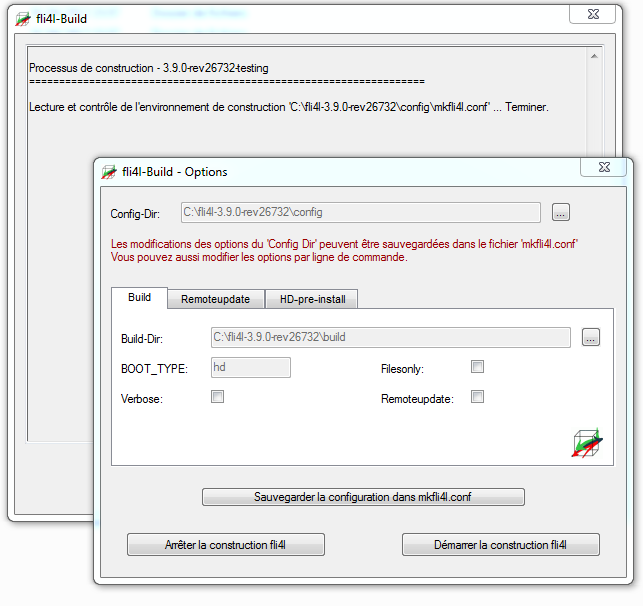
\includegraphics[width=\columnwidth]{win_build_build}
  \caption{Paramètre}
  \label{fig:win_build_build}
  \end{figure}

  On défini dans cette fenêtre, la sauvegarde des paramètres et la création du média~:
  \begin{itemize}
    \item Build-Dir~-- Répertoire pour l'archive/l'image CD/...
    \item \var{BOOT\_TYPE}~-- Régle l'affichage/utilisé \var{BOOT\_TYPE}~-- il ne peut pas être modifié ici
    \item Verbose~--- Affiche les informations pendant la construction du programme fli4l
    \item Filesonly~--- Sauvegarde uniquement les fichiers, pas de création d'image
    \item Remoteupdate~--- Active la mise à jour par SCP
  \end{itemize}

  Avec le bouton \textbf{les paramètres du programme fli4l-build peuvent être sauvegardés à tout moment},
       les paramètres seront enregistrés dans le fichier mkfli4l.txt, ils
       peuvent être modifié manuellement en ouvrant ce fichier.


  \subsection{Boîte de dialogue~-- Paramètres pour la mise à jour à distance}
  \begin{figure}[h!]
  \centering
  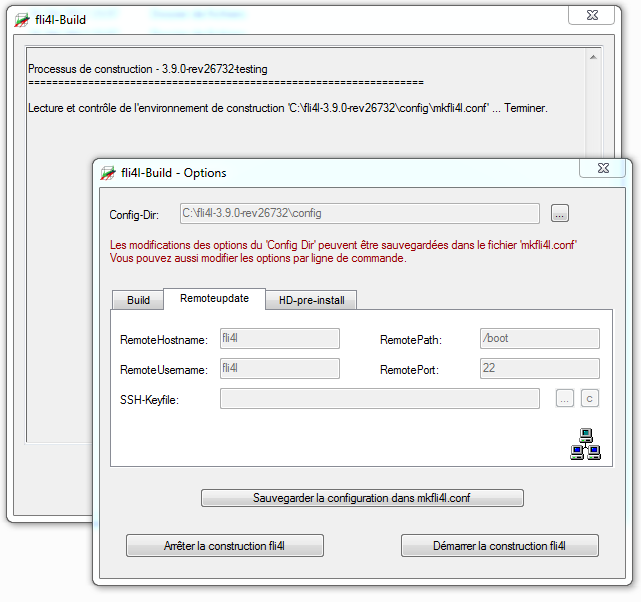
\includegraphics[width=\columnwidth]{win_build_remoteupdate}
  \caption{Paramètre pour la mise à jour}
  \label{fig:win_build_remoteupdate}
  \end{figure}

  On défini dans cette fenêtre, les réglages pour l'installation d'une mise à jour~:
  \begin{itemize}
    \item Adresse IP ou Nom d'Hôte
    \item Nom d'utilisateur sur l'hôte distant
    \item Remote-path (Par défaut: /boot)
    \item Remote-port (Port par défaut: 22)
    \item Utiliser SSH-Keyfile (Format ppk de Putty)
  \end{itemize}

  \subsection{Boîte de dialogue~-- Paramètres pour une pré-installation du HD}
  \begin{figure}[h!]
  \centering
  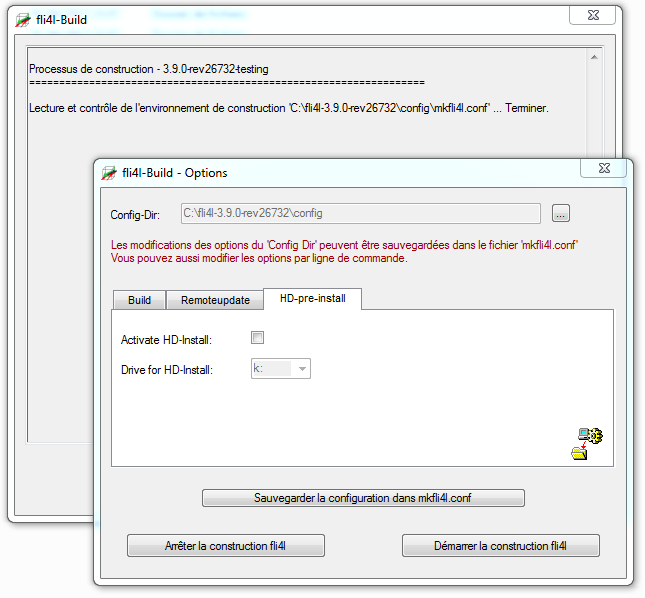
\includegraphics[width=\columnwidth]{win_build_hd_install}
  \caption{Paramètre pour pré-installation du DD}
  \label{fig:win_build_hd_install}
  \end{figure}

   On défini dans cette fenêtre, les paramètres pour la pré-installation
   d'un disque dur, une Carte CompactFlash, une clef USB formaté et partitionné.

   Options possibles~:
  \begin{itemize}
     \item Active la pré-installation du Disque Dur
     \item Lettre du lecteur ou de la Carte-CF
  \end{itemize}

  Information pour partitionner et formater CF (Compact Flash)~: Pour
  cette installation utiliser le TYPE A, de plus (nous avons besoin
  du paquetage HD), une partition FAT primaire doit être active et
  formatée sur la CF. Si l'on veut utiliser une partition bootable
  il faut installer une partition Linux supplémentaire formatée avec
  le système ext3, on aura besoin du fichier \texttt{hd.cfg} sur la partition
  FAT (pour cela il faut absolument installer et configurer le paquetage HD).


\marklabel{sec:mkfli4lconf}{
  \section{Paramètre pour le fichier mkfli4l.txt}}

  Il existe depuis la Version fli4l 2.1.9, le fichier de
  configuration \texttt{$<$config$>$/mkfli4l.txt}. Toutes les commandes
  du programme 'graphique' fli4l-Build sont enregistrées dans
  le fichier mkfli4l.txt. Le fichier est construit comme tous
  les fichiers fli4l. Toutes les variables de configuration sont
  optionnelles, mais il ne faut pas, modifier les variables spécifiques.

  \begin{description}

  \config {BUILDDIR}{BUILDDIR}{BUILDDIR}

  Valeur par défaut~: 'build'

  On indique ici le nom du répertoire pour enregistrer les fichiers de
  construction pour le boot de fli4l. Si la variable n'est pas définie, mkfli4l
  sous Windows utilisera par défaut le sous-répertoire \texttt{build} de la racine
  du répertoire fli4l~:
  \begin{verbatim}
     Chemin/fli4l-x.y.z/build
  \end{verbatim}
  \vspace{-2ex}
  En lancant mkfli4l le programme enregistre des fichiers de
  construction produits dans le répertoire \texttt{$<$config$>$/build}.

  Vous devez utiliser les conventions des systèmes d'exploitation de Windows ou
  *Unix pour paramétrer le chemin d'accès \var{BUILDDIR}. Si vous avez paramétré
  un chemin relatif, ce chemin sera converti par le processus de construction
  de Windows ou *Unix.

  \config {VERBOSE}{VERBOSE}{VERBOSE}

  Valeur par défaut~: \var{VERBOSE='no'}

  Valeurs possibles sont \var{'yes'} ou \var{'no'}. Affiche les
  \emph{les Informations} du processus Build (ou processus de construction).

  \config {FILESONLY}{FILESONLY}{FILESONLY}

  Valeur par défaut~: \var{FILESONLY='no'}

  Valeurs possibles \var{'yes'} ou \var{'no'}. Vous permet de créer un Boot
  média, peut être désactivé de sorte à créer uniquement les fichiers d'archives.

  \config {REMOTEUPDATE}{REMOTEUPDATE}{REMOTEUPDATE}

  Valeur par défaut~: \var{REMOTEUPDATE='no'}

  Valeurs possibles \var{'yes'} ou \var{'no'}. Si on veut transmettre
  automatiquement des fichiers de boot sur le Routeur au moyen de SCP.
  Cela suppose que le paquetage \jump{OPTSSHD}{SSHD} est installé et
  en plus la variable \texttt{scp} soit activée dans se paquetage.

  \config {REMOTEHOSTNAME}{REMOTEHOSTNAME}{REMOTEHOSTNAME}

  Valeur par défaut~: \var{REMOTEHOSTNAME=''}

  On indique ici le nom d'hôte du destinataire pour le transfert des
  données avec SCP. Si vous n'avez indiqué aucun nom, le nom de la
  variable \jump{HOSTNAME}{\var{HOSTNAME}} est utilisée pour le
  transfert des données.

  \config {REMOTEUSERNAME}{REMOTEUSERNAME}{REMOTEUSERNAME}

  Valeur par défaut~: \var{REMOTEUSERNAME='fli4l'}

  Nom d'utilisateur pour la transmission des données SCP.

  \config {REMOTEPATHNAME}{REMOTEPATHNAME}{REMOTEPATHNAME}

  Valeur par défaut~: \var{REMOTEPATHNAME='/boot'}

  Chemin d'accès du destinataire pour la transmission des données SCP.

  \config {REMOTEPORT}{REMOTEPORT}{REMOTEPORT}

  Valeur par défaut~: \var{REMOTEPORT='22'}

  Port du destinataire pour la transmission des données SCP.

  \config {SSHKEYFILE}{SSHKEYFILE}{SSHKEYFILE}

  Valeur par défaut~: \var{SSHKEYFILE=''}

  Ici on peut indiquer le fichier de clef-SSH pour la mise à jour
  avec SCP. Un mot de passe peut aussi être demandé pour la mise à jour.

  \config {REMOTEREMOUNT}{REMOTEREMOUNT}{REMOTEREMOUNT}

  Valeur par défaut~: \var{REMOTEREMOUNT='no'}

  Les valeurs possibles sont \var{'yes'} ou \var{'no'}. Si vous indiquez
  \var{'yes'}, vous remontez le boot device "/boot" en lecture/écriture
  si le boot est en lecture seule, c'est pour monter et rendre possible
  la mise à jour distante.

  \config {TFTPBOOTPATH}{TFTPBOOTPATH}{TFTPBOOTPATH}

  Le chemin d'accès pour installer l'image de boot par le réseau.

  \config {TFTPBOOTIMAGE}{TFTPBOOTIMAGE}{TFTPBOOTIMAGE}

  Nom de l'image de boot sur le réseau.

  \config {PXESUBDIR}{PXESUBDIR}{PXESUBDIR}

  Sous-répertoire pour les fichiers PXE qui est en rapport avec TFTPBOOTPATH.

  \config {SQUEEZE\_SCRIPTS}{SQUEEZE\_SCRIPTS}{SQUEEZESCRIPTS}

  Active ou désactive Squeeze (compression des scripts). Par ex. un
  Script qui contient en plus des lignes de commentaires, ces lignes
  serons supprimées à la compressé par Squeeze. Normalement on devrais
  toujours indiquer \var{'yes'} dans cette variable.

  \config {MKFLI4L\_DEBUG\_OPTION}{MKFLI4L\_DEBUG\_OPTION}{MKFLI4LDEBUGOPTION}

   Options supplémentaires de débugage, peut être transmis au \jump{mkfli4l}{Programme-mkfli4l}.

  \end{description}

  \chapter{Réglage des PCs dans le LAN}

  Réglage des ordinateurs dans le LAN (ou réseau local)~:

  \begin{enumerate}
  \item Adresse IP (voir \smalljump{sec:pc-lan-ip}{Adresse IP})
  \item Nom de l'ordinateur et Nom de Domaine
    (voir \smalljump{sec:pc-lan-name}{Nom de l'ordinateur et de Domaine})
  \item Gateway-Standard (Passerelle Standard) (voir \smalljump{sec:pc-lan-gateway}{Gateway})
  \item Adresse IP et serveur-DNS (voir \smalljump{sec:pc-lan-dns}{Serveur-DNS})
  \end{enumerate}


  \marklabel{sec:pc-lan-ip}{\section{Adresse IP}}
  Les adresses IP du réseau local doivent se trouver dans le même
  réseau que l'adresse IP du routeur fli4l (de l'interface Ethernet),
  par ex. 192.168.6.2 pour l'ordinateur local dans le cas ou le routeur
  aurait l'adresse IP 192.168.6.1. Les adresses IP doivent être uniques
  dans le réseau, changer uniquement le dernier chiffre de l'adresse IP
  est un bon moyen pour ne pas se tromper. Vous devez vous assurez que
  l'adresses IP indiqué ici est la même adresse IP que vous avez config
  pour cet ordinateur dans le fichier config/base.txt.

  \marklabel{sec:pc-lan-name}{\section{Nom de l'ordinateur et de domaine}}
  Le nom de l'ordinateur est par ex. "mon-pc", et le nom de Domaine "lan.fli4l".

  \wichtig{Le domaine qui est réglé dans le PC doit être identique
   au domaine choisi dans l'ordinateur fli4l, si on veut utiliser le
   routeur fli4l comme serveur DNS, il peut y avoir d'énormes problèmes
   dans le réseau si les domaines sont différents.}

  La raison~: les ordinateurs Windows cherchent régulièrement les
  ordinateurs avec le même nom de groupe de travail WORKGROUP.mon-domain.fli4l.
  Si fli4l ne répond pas à la requête du domaine (ici~: mon-domain.fli4l),
  alors fli4l essayera de chercher le domaine en se connectant sur Internet \ldots

  Le domaine doit être enregistré dans les réglages TCP/IP de l'ordinateur.

  \subsection{Windows 2000}

  Pour Windows 2000 se trouve sous~:

  \noindent Démarrer \pfeil\\
  \hspace*{2ex}Paramètre \pfeil\\
  \hspace*{4ex}Panneau de configuration \pfeil\\
  \hspace*{6ex}Connexion réseau \pfeil\\
  \hspace*{8ex}Connexion au réseau local \pfeil\\
  \hspace*{10ex}Bouton droit propriétés  \pfeil\\
  \hspace*{12ex}Protocole Internet (TCP/IP) \pfeil\\
  \hspace*{14ex}Sélectionner \pfeil\\
  \hspace*{16ex}Avancé \ldots \pfeil\\
  \hspace*{18ex}DNS \pfeil\\
  \hspace*{20ex}Suffix DNS pour cette connexion \pfeil\\

  Entrer "lan.fli4l" (ou indiquer votre domaine) (sans les "" !)
  \pfeil et appuyez sur OK.

\subsection{NT 4.0}

  Démarrer \pfeil\\
  \hspace*{2ex}Paramètre \pfeil\\
  \hspace*{4ex}Panneau de configuration  \pfeil\\
  \hspace*{6ex}Réseau \pfeil\\
  \hspace*{8ex}Protocole \pfeil\\
  \hspace*{10ex}TCP/IP \pfeil\\
  \hspace*{12ex}Propriétés \pfeil\\
  \hspace*{14ex}DNS \pfeil\\
  \hspace{16ex}\begin{itemize}
  \item Nom d'hôte entrer (le Nom de l'ordinateur)
  \item Domaine entrer (le même Nom que dans le fichier config/base.txt)
  \item Ajouter adresse IP le même réseau que le routeur fli4l
  \item Ajouter suffix DNS (Domaine le même que la ligne 2)
  \end{itemize}

\subsection{Windows 95/98}

  Démarrer \pfeil\\
  \hspace*{2ex}Paramètre \pfeil\\
  \hspace*{4ex}Panneau de configuration \pfeil\\
  \hspace*{6ex}Réseau \pfeil\\
  \hspace*{8ex}Configuration \pfeil\\
  \hspace*{10ex}TCP/IP (sélectionner la carte réseau qui va au routeur) \pfeil\\
  \hspace*{12ex}propriétés \pfeil\\
  \hspace*{14ex}Configuration DNS~:

  Cliquer activé DNS, dans le champ "Domaine"~: entrer "lan.fli4l"
  (ou indiquer votre domaine) (sans les "" !).

\subsection{Windows XP}

  Pour Windows XP se trouvent sous~:

  \noindent Démarrer \pfeil\\
  \hspace*{2ex}Paramètre \pfeil\\
  \hspace*{4ex}Panneau de configuration \pfeil\\
  \hspace*{6ex}Connexions réseau \pfeil\\
  \hspace*{8ex}Connexion au réseau local \pfeil\\
  \hspace*{10ex}Propriétés \pfeil\\
  \hspace*{12ex}Protocole Internet (TCP/IP) \pfeil\\
  \hspace*{14ex}Propriétés \pfeil\\
  \hspace*{16ex}Avancé\ldots \pfeil\\
  \hspace*{18ex}DNS \pfeil\\
  \hspace*{20ex}Suffixe DNS pour cette connexion \pfeil\\

  Indiquez "lan.fli4l" (ou indiquer votre domaine) (sans les "" !)
  \pfeil Cliquez sur OK.

  \subsection{Windows 7}

  Pour Windows 7 se trouvent sous~:

  \noindent Bouton Windows (ex. Démarrer) \pfeil\\
  \hspace*{2ex}Contrôle \pfeil\\
  \hspace*{4ex}Panneau de configuration \pfeil\\
  \hspace*{6ex}Centre Réseau et partage \pfeil\\
  \hspace*{8ex}Connexion au réseau local \pfeil\\
  \hspace*{10ex}Propriétés \pfeil\\
  \hspace*{12ex}Protocole Internet version 4 (TCP/IPv4) \pfeil\\
  \hspace*{14ex}Propriétés \pfeil\\
  \hspace*{16ex}Avancé\ldots \pfeil\\
  \hspace*{18ex}DNS \pfeil\\
  \hspace*{20ex}Suffixe DNS pour cette connexion \pfeil\\

  Indiquez "lan.fli4l" (ou indiquer votre domaine) (sans les "" !)
  \pfeil Cliquez sur OK.

\subsection{Windows 8}

  Pour Windows 8 se trouvent sous~:

  \noindent Appuyez simultanément sur la touche Windows et X \pfeil\\
  \hspace*{2ex}Contrôle \pfeil\\
  \hspace*{4ex}Connexions réseau \pfeil\\
  \hspace*{6ex}Sélectionnez votre réseau (Ehternet ou WLAN) \pfeil\\
  \hspace*{8ex}Clique droit \pfeil\\
  \hspace*{10ex}Propriétés \pfeil\\
  \hspace*{12ex}Protocole Internet version 4 (TCP/IPv4) \pfeil\\
  \hspace*{14ex}Propriétés \pfeil\\
  \hspace*{16ex}Avancé\ldots \pfeil\\
  \hspace*{18ex}DNS \pfeil\\
  \hspace*{20ex}Suffixe DNS pour cette connexion \pfeil\\

  Indiquez "lan.fli4l" (ou indiquer votre domaine) (sans les "" !)
  \pfeil Cliquez sur OK.

  \marklabel{sec:pc-lan-gateway}{\section{Gateway (ou Passerelle)}}

  Il est absolument nécessaire d'indiquer une adresse IP dans le paramètre
  passerelle par défaut de votre PC, car s'il n'y a pas d'adresse IP d'indiquée,
  rien ne fonctionnera. Ainsi vous devrez indiquer l'adresse IP du routeur
  fli4l - (Interface Ethernet) par exemple 192.168.6.4, selon l'adresse
  IP qui est configurée dans le fichier config/base.txt du routeur fli4l.

  Il est incorrect de configuter le routeur fli4l comme un proxy dans Windows
  ou dans de votre navigateur~-- sauf si vous définissez un proxy sur votre
  routeur fli4l. Normalement fli4l a pas de proxy, s'il vous plaît ne spécifiez
  \emph{pas} fli4l comme un proxy~!

\marklabel{sec:pc-lan-dns}{\section{Serveur DNS}}

  Pour l'adresse IP du serveur DNS, vous ne devez pas indiquer
  d'adresse IP de votre fournisseur d'accés Internet mais l'adresse IP
  du routeur (interface Ethernet), car le routeur peut répondre aux
  requêtes DNS et faire suivre ceux-ci par Internet si nécessaire.

  Quand fli4l est utilisé comme serveur DNS, beaucoup de requêtes
  DNS son envoyées par les PCs client Windows, c'est le routeur fli4l qui
  leur répond directement, elles ne sont pas expédiées sur Internet.

\marklabel{sec:pc-lan-misc}{\section{Divers points }}

  Les points 1 et 4 n'ont pas besoin d'être enregistrés avec un
  serveur DHCP puisque le routeur fli4l communique les données
  nécessaires automatiquement.

  \textbf{Dans Options Internet~:} et dans la fenètre connexion vous ne devez
  "sélectionner aucun lien". Dans Paramètre réseau local (LAN)~: ne RIEN
  indiquer (sauf si vous utilisez le paquetage \var{OPT\_\-P}roxy).
  Par défaut les deux paramètres n'ont pas besoin d'être modifié pour
  une utilisation normale.


  \marklabel{IMONDSCHNITTSTELLE}{
    \chapter{Interface client/serveur imon}
  }

  \marklabel{sec:imond}{
    \section{Server imon avec imond}}

  Imond est un programme serveur qui répond à certaines enquêtes sur
  la gestion du réseau et accepte aussi des commandes qui peuvent contrôler
  le routeur sur le réseau local.

  Imond contrôle également les Moindres-Coûts-Routages. Il utilise
  le fichier de configuration /etc/imond.conf qui est produit
  automatiquement au moment du boot, à partir de la variable \var{ISDN\_\-CIRC\_\-x\_\-XXX}
  du fichier config/isdn.txt, le fichier est généré par un script shell.

  imond est un démon qui fonctionne en permanence en tache de fond,
  il écoute le port 5000 TCP/IP sur le périphérique /dev/isdninfo.

  Voici toutes les commandes qui peuvent être envoyées par le port 5000 TCP/IP~:
  \begin{table}
    \textbf{Commandes Admin}

    \vspace{1ex}
    \begin{tabular}{lp{9cm}}

      addlink ci-index              & Ajouter un canal au circuit (Channel-Bundling) \\
      adjust-time seconds           & Incrémente la date sur le routeur en secondes \\
      delete filename pw            & Supprime le fichier sur le routeur \\
      hup-timeout \#ci-index [value]& Affiche ou compose le HUP-Timeout pour
                                      des circuits RNIS (ou numéris) \\
      removelink ci-index           & Enlever le canal supplémentaire \\
      reset-telmond-log-file        & Supprime le fichier journal de telmond \\
      reset-imond-log-file          & Supprime le fichier journal de imond \\
      receive filename \#octets pw  & Transfére d'un fichier au routeur.
                                      Imond donne l'ordre avec ACK (0x06). Après,
                                      le fichier est transféré par blocs de 1024
                                      Octets qui sont également confirmé avec ACK.
                                      En conclusion, imond répond OK. \\
      send filename pw              & Si le mot de passe est correct et que le
                                      fichier existe, imond répond OK avec un \#octet.
                                      Puis, imond transfère le fichier par blocs de
                                      1024 octets, chaque fois confirmés avec ACK
                                      (0x06). A la fin, imond répond OK. \\
      support pw                    & Montre le statut/configuration du routeur \\
      sync                          & Synchronise le Cache des lecteurs montés \\
    \end{tabular}
  \end{table}


  \begin{table}
    \textbf{Commandes Admin et Utilisateur}

    \vspace{1ex}
    \begin{tabular}{lp{9cm}}

      dial                      &    Choix du FAI (Defaut-Route-Circuit) \\
      dialmode [auto|manual|off]&    Réglage des actions dans Dialmode \\
      disable                   &    Raccroche et place dialmode sur "off" \\
      enable                    &    Mets dialmode sur "auto" \\
      halt                      &    Descend proprement le Routeur \\
      hangup [\#channel-id]     &    Raccroche \\
      poweroff                  &    Descent le routeur et mise hors tension \\
      reboot                    &    Reboot le routeur fli4l! \\
      route [ci-index]          &    Met le routeur par Defaut sur un Circuit X (0=automatique) \\
    \end{tabular}
  \end{table}


  \begin{table}
    \textbf{Commandes Utilisateur}

    \vspace{1ex}
    \begin{tabular}{lp{9cm}}
      channels                  & Nombre de Canaux ISDN disponibles \\
      charge \#channel-id       & Edite les frais de connexion pour un Canal en ligne \\
      chargetime \#channel-id   & Temps et frais de connexion pour un canal en ligne \\
      circuit [ci-index]        & Edite le numéro du Circuit \\
      circuits                  & Edite le nombre de Defaut-Route-Circuits \\
      cpu                       & Donne la charge du CPU en pourcentage \\
      date                      & Edite la date et heure \\
      device ci-index           & Circuits du périphérique utilisé \\
      driverid \#channel-id     & Edite Driver-ID pour le Canal X \\
      help                      & Edite l'aide \\
      inout \#channel-id        & Edite la direction (entrante/sortante) \\
      imond-log-file            & Edite le fichier du Protocole imond \\
      ip \#channel-id           & Edite l'adresse IP \\
      is-allowed command        & Edite si la commande est valide\newline
                                  commandes possibles~:
                                  dial|dialmode|route|reboot
                                  |imond-log|telmond-log|mgetty-log \\
      is-enabled                & Edite si dialmode est sur off (0) ou auto (1) \\
      links ci-index            & Edite le nombre de canaux 0, 1 ou 2, 0 utilisé,
                                  ou alors~: Aucun Channel-Bundling possible \\
      log-dir imond|telmond|mgetty& Donne la direction des fichiers Log \\
      mgetty-log-file           & Edite le protocole du fichier mgetty \\
      online-time \#channel-id  & Edite le temps en ligne, et de connexion en hh:mm:ss \\
      pass [password]           & Vérifie, le mot de passe qui a été saisit par\newline
                                  1 Mot de passe Utilisateur est fixé\newline
                                  2 Mot de passe Admin est fixé\newline
                                  4 imond se trouve dans le mode Admin \\
      phone \#channel-id        & Edite le numéro de Tél et le nom du "correspondant" \\
      pppoe                     & Donne le numéro du périphérique pppoe (0 ou 1) \\
      quantity \#channel-id     & Donne l'ensemble des transmissions (en octet) \\
      quit                      & Coupe la connexion avec imond \\
      rate \#channel-id         & Edite les connexions (entrant/sortant en Octet/sec) \\
      status \#channel-id       & Edite le statut pour le Canal X \\
      telmond-log-file          & Edite le protocole telmond \\
      time \#channel-id         & Edite le temps total en ligne, au Format hh:mm:ss \\
      timetable [ci-index]      & Edite la time-table LC-Routing \\
      uptime                    & Edite le temps d'utilisation du Routeur en secondes \\
      usage \#channel-id        & Edite les réponses des connexions: Fax, Répondeur, Net, Modem, Raw \\
      version                   & Edite la version du protocole et la version du Programme \\
    \end{tabular}
  \end{table}


  Le port 5000 TCP/IP est accessible uniquement depuis un réseau LAN
  masqué. Avec la configuration standard du firewall l'accés est bloqué
  de l'extérieur.

  Imond supporte deux modes d'administrations, le Mode Utilisateur et
  le Mode Admin. On peut installer un Mot de Passe pour ces deux modes
  au moyen des variables \var{IMOND\_\-PASS} et \var{IMOND\_ADMIN\_\-PASS}.
  Si le Mot de Passe n'est pas transmis au serveur imond le client imonc
  a accés uniquement à deux commandes "pass" et "quit" toutes les autres
  commandes sont rejetées et une erreur s'affiche.

  Si plus tard, vous voulez limiter l'accés au serveur imond à un seul PC,
  la configuration du Firewall doit être modifier.

  Les commandes

\begin{example}
\begin{verbatim}
         enable/disable/dialmode   dial/hangup   route   reboot/halt
\end{verbatim}
\end{example}

  peuvent être activées ou désactivées dans la variable
  \var{IMOND\_\-XXX} voir (le chapitre "configuration").

  Avec un ordinateur Unix/Linux (ou un ordinateur Windows par la
  fenètre DOS) vous pouvez facilement entrer les commandes aprés
  la connexion telnet.

  Connexion telnet~:

\begin{example}
\begin{verbatim}
        telnet fli4l 5000        \# ou le Nom correspondant au routeur fli4l
\end{verbatim}
\end{example}

  Vous pouvez directement entrer les commandes mentionnées ci-dessus.

  Par exemple la commande "help" active l'aide sur l'écran ou "quit"
  démonte (ou arrête) le serveur imond.

\marklabel{sec:leastcostrouting}{
  \subsection{Mode de fonctionnement du Moindre-Coût-Routage}
  }

  imond construit une Time-Table (ou Plage Horaire) à partir du fichier
  de configuration /etc/imond.conf (qui est créé au boot avec la variable
  de configuration \var{ISDN\_\-CIRC\_\-x\_\-TIMES}. Ce "calendrier" est
  composé d'une semaine par intervalle d'une heure, une semaine = 168
  heures = 168 octets. La table se compose de circuits, dans lesquel sont
  définis des Défaut-Routes (ou connexion par défaut au FAI).

  Avec la commandement "timetable" on peut voir la table imond.
  Exemple de configuration~:

Supposons que nous définissions 3 circuits de connexions pour chaque FAI c'est à dire~:

\begin{example}
\begin{verbatim}
        CIRCUIT_1_NAME='Addcom'
        CIRCUIT_2_NAME='AOL'
        CIRCUIT_3_NAME='Firma'
\end{verbatim}
\end{example}

  Les deux premiers circuits sont réglés avec Défaut-Route c.à d.
  que l'itinétaire par défaut est écrit dans la variable
  ISDN\_CIRC\_x\_ROUTE avec la valeur '0.0.0.0/0'.

  Les variables \var{ISDN\_\-CIRC\_\-x\_\-TIMES} se présentent de la manière suivante~:

\begin{example}
\begin{verbatim}
        ISDN_CIRC_1_TIMES='Mo-Fr:09-18:0.0388:N Mo-Fr:18-09:0.0248:Y
                      Sa-Su:00-24:0.0248:Y'

        ISDN_CIRC_2_TIMES='Mo-Fr:09-18:0.019:Y Mo-Fr:18-09:0.049:N
                      Sa-Su:09-18:0.019:N Sa-Su:18-09:0.049:N'

        ISDN_CIRC_3_TIMES='Mo-Fr:09-18:0.08:N Mo-Fr:18-09:0.03:N
                      Sa-Su:00-24:0.03:N'
\end{verbatim}
\end{example}

  Puis le fichier /etc/imond.conf est créé de cette façon~:

\begin{example}
\begin{verbatim}
        #day  hour  device  defroute  phone        name        charge  ch-int
        Mo-Fr 09-18 ippp0   no        010280192306 Addcom      0.0388   60
        Mo-Fr 18-09 ippp0   yes       010280192306 Addcom      0.0248   60
        Sa-Su 00-24 ippp0   yes       010280192306 Addcom      0.0248   60
        Mo-Fr 09-18 ippp1   yes       019160       AOL         0.019   180
        Mo-Fr 18-09 ippp1   no        019160       AOL         0.049   180
        Sa-Su 09-18 ippp1   no        019160       AOL         0.019   180
        Sa-Su 18-09 ippp1   no        019160       AOL         0.049   180
        Mo-Fr 09-18 isdn2   no        0221xxxxxxx  Firma       0.08     90
        Mo-Fr 18-09 isdn2   no        0221xxxxxxx  Firma       0.03     90
        Sa-Su 00-24 isdn2   no        0221xxxxxxx  Firma       0.03     90
\end{verbatim}
\end{example}

  imond produit alors Time-Table (ou Plage Horaire) dans la mémoire.
  voici la table des données sorties avec la commande "timetable"~:

\begin{example}
\begin{verbatim}
         0  1  2  3  4  5  6  7  8  9 10 11 12 13 14 15 16 17 18 19 20 21 22 23
     --------------------------------------------------------------------------
     Su  3  3  3  3  3  3  3  3  3  3  3  3  3  3  3  3  3  3  3  3  3  3  3  3
     Mo  2  2  2  2  2  2  2  2  2  4  4  4  4  4  4  4  4  4  2  2  2  2  2  2
     Tu  2  2  2  2  2  2  2  2  2  4  4  4  4  4  4  4  4  4  2  2  2  2  2  2
     We  2  2  2  2  2  2  2  2  2  4  4  4  4  4  4  4  4  4  2  2  2  2  2  2
     Th  2  2  2  2  2  2  2  2  2  4  4  4  4  4  4  4  4  4  2  2  2  2  2  2
     Fr  2  2  2  2  2  2  2  2  2  4  4  4  4  4  4  4  4  4  2  2  2  2  2  2
     Sa  3  3  3  3  3  3  3  3  3  3  3  3  3  3  3  3  3  3  3  3  3  3  3  3

     No.  Name                   DefRoute  Device  Ch/Min   ChInt
      1   Addcom                   no      ippp0   0.0388     60
      2   Addcom                   yes     ippp0   0.0248     60
      3   Addcom                   yes     ippp0   0.0248     60
      4   AOL                      yes     ippp1   0.0190    180
      5   AOL                      no      ippp1   0.0490    180
      6   AOL                      no      ippp1   0.0190    180
      7   AOL                      no      ippp1   0.0490    180
      8   Firma                    no      isdn2   0.0800     90
      9   Firma                    no      isdn2   0.0300     90
     10   Firma                    no      isdn2   0.0300     90
\end{verbatim}
\end{example}

  Pour le circuit 1 (Addcom) il y a trois éléments définis (1-3),
  pour le circuit 2 il y a quatre éléments (4-7), et pour le circuit 3
  il y a trois éléments (8-10).

  Les index des circuits activés sont inscris toutes les heures dans
  la Time-Table respectivement. Ici les index (2-4) apparaissent,
  car les autres ne passent pas par LC-Défaut-Route.

  Si vous avez des zéros dans Time-Table, c'est qu'il manque des données
  dans la variable \var{ISDN\_\-CIRC\_\-X\_\-TIMES}. Si vous avez des
  zéro sur certaine plage horaire, cela veux dire qu'il n'y aura pas de
  Défaut-Route et aucun accés Internet possible sur ces plages horaires!

  Au démarrage du programme, imond vérifie le jour de la semaine et
  l'heure, puis les index dans la Time-Table et enfin régle les Défauts-Routes
  correspondants. Le Défaut-Route (ou connexion par Défaut au FAI) est alors
  activé par rapport à l'indexation.

  Lors d'un changement de statut, par exemple sur un canal, une connexion
  ou un racrochement de la ligne, si la commande mais plus d'une minute,
  le processus de démarrage est réactualisé, vérification de l'horaire et
  du jour, consultation de la table, selection du Circuit-Défaut-route.

  Si par exemple le lundi à 18:00 la connexion change, Défaut-Route est
  supprimé, les connexions existantes sont arrêtées (désolé\ldots),
  ensuite imond controle dans la Time-Table si un nouveau Circuit-Défaut-route
  existe, si oui imond mettra environ 60 secondes pour se reconnecter.
  Donc la connexion se fera au plus tard à 18:00:59.

  Il n'y aura aucun changement pour les circuits qui n'utilisent pas
  un Defaut-Route. Le contenu \var{ISDN\_\-CIRC\_\-x\_\-TIMES} sera
  uniquement employé pour le calcul des frais téléphoniques. Ceci peut
  être pertinent, si vous arrêtez temporairement le client imonc et que
  vous choisissiez manuellement un Circuit-Défaut-route.

  Vous pouvez également regarder dans l'indexation de Time-Table (exemple
  précédent de 1 à 10) les circuits non activés "Non-LC-Default-Route-Circuits".

  Commande pour vérifier un index dans le Time-Table~:

\begin{example}
\begin{verbatim}
                    timetable "index"
\end{verbatim}
\end{example}

  Exemple~:

\begin{example}
\begin{verbatim}
                    telnet fli4l 5000
                    timetable 5
                    quit
\end{verbatim}
\end{example}

  La sortie des données apparaîtront comme ceci~:

\begin{example}
\begin{verbatim}
         0  1  2  3  4  5  6  7  8  9 10 11 12 13 14 15 16 17 18 19 20 21 22 23
     --------------------------------------------------------------------------
     Su  0  0  0  0  0  0  0  0  0  0  0  0  0  0  0  0  0  0  0  0  0  0  0  0
     Mo  5  5  5  5  5  5  5  5  5  0  0  0  0  0  0  0  0  0  5  5  5  5  5  5
     Tu  5  5  5  5  5  5  5  5  5  0  0  0  0  0  0  0  0  0  5  5  5  5  5  5
     We  5  5  5  5  5  5  5  5  5  0  0  0  0  0  0  0  0  0  5  5  5  5  5  5
     Th  5  5  5  5  5  5  5  5  5  0  0  0  0  0  0  0  0  0  5  5  5  5  5  5
     Fr  5  5  5  5  5  5  5  5  5  0  0  0  0  0  0  0  0  0  5  5  5  5  5  5
     Sa  0  0  0  0  0  0  0  0  0  0  0  0  0  0  0  0  0  0  0  0  0  0  0  0

     No.  Name                   DefRoute  Device  Ch/Min   ChInt
      5   AOL                      no      ippp1   0.0490    180
\end{verbatim}
\end{example}

  Tout est clair jusque là~?

  Avec la commande "Route" d'imond vous pouvez commuter "Marche/Arrêt"
  de LC-Routing, et vous pouvez indiquer l'index du Circuit-Défaut-Route
  (1\ldots N), il se connectera sur le circuit. Si l'index est 0, le
  LC-Routing est activé et le circuit sera choisi automatiquement.

  \subsection{Calcul des frais on-line (en ligne)}

  Le mode de calcul des frais de connexions fonctionnera correctement
  uniquement si l'unité téléphonique est constante tout au long
  de la semaine, elle doit est inscrit dans la variable
  \var{ISDN\_\-CIRC\_\-x\_\-CHARGEINT}) en seconde. Normalement c'est la
  régle pour les fournisseurs d'accés Internets. Toutefois, si vous choisissez
  Telekom (je ne parle pas de T-Online~!) par exemple, pour un réseau
  d'entreprise, qui sera considéré comme des conversations téléphoniques normales.
  et changement passe de 90 secondes à 4 minutes aprés 18:00 (Stand Juni
  00). Par conséquent, la définition

   Mais si vous utilisez votre
  société téléphonique par exemple pour un accés Internet avec TéléKom
  (Allemagne) l'unité Tél change (information juin 2000).\\
  En France l'unité Tél est toujours constante 60 secondes, on n'a
  pas ce problème, c'est juste le tarif qui change en heure creuse
  0,018 euro et en heure pleine 0,033 euro (8:00 à 19:00 heure pleine).

\begin{example}
\begin{verbatim}
        ISDN_CIRC_3_CHARGEINT='90'
        ISDN_CIRC_3_TIMES='Mo-Fr:09-18:0.08:N Mo-Fr:18-09:0.03:N Sa-Su:00-24:0.03:N'
\end{verbatim}
\end{example}

  est en fait pas tout à fait exact. Le tarif le soir est de 3 cents la minute
  (donc 12 cents les 4 minutes de télécommunication), mais la mesure est fausse.
  C'est pour cette raison qu'il se produit des différences d'affichage par
  rapport au prix réel.

  Il est possible que ce problème soit peut être corrigé plus tard.
  En attendant on peut définir dans la variable \var{ISDN\_\-CIRC\_\-x\_\-CHARGEINT})
  2 Circuits~: un pour la journée avec \var{ISDN\_\-CIRC\_\-1\_\-CHARGEINT}='90'
  et l'autre pour la soirée \var{ISDN\_\-CIRC\_\-2\_\-CHARGEINT}='240'
  naturellement vous devez configurer \var{ISDN\_\-CIRC\_\-x\_\-TIMES},
  avec cette configuration vous utiliser le Circuit 1 pendant la journée
  et le Circuit 2 en soirée.

  Comme nous l'avons dit plus haut~: l'utilisation des connexions avec
  un fournisseur d'accés Internet, ne pose pas de problème parce que
  l'unité Tél est toujours constante et le coût par minute ne change pas
  (il a encore quelque chose? je ne fais pas confiance à T-* pour tout :-).


  % Last Update: $Id$
  \marklabel{sec:winimonc}{
    \section{Windows-Client imonc.exe}}

  \subsection{Einleitung}

  Das Gespann imond auf dem Router und imonc auf dem Client beherrschen
  zwei Benutzermodi: den User- und den Adminmodus. Im Adminmodus sind alle
  Steuerelemente aktiviert. Im Usermodus steuern die Variablen 
  \jump{IMONDENABLE}{\var{IMOND\_ENABLE}}, \jump{IMONDDIAL}{\var{IMOND\_DIAL}}, 
  \jump{IMONDROUTE}{\var{IMOND\_ROUTE}} und \jump{IMONDREBOOT}{\var{IMOND\_REBOOT}} ob die
  jeweiligen Funktionen im Usermodus zur Verfügung stehen. Sind alle diese 
  Variablen auf `no' gesetzt, bedeutet dies für die Überblick-Seite, dass alle 
  Buttons bis auf den Exit- und den Admin-Mode-Button deaktiviert sind. Die 
  Entscheidung, ob der User- oder Admin-Modus benutzt wird, wird anhand des 
  übermittelten Passwortes getroffen. Über den Button Admin-Mode, der sich in 
  der Statusleiste befindet, kann jederzeit unter Eingabe des Admin-Passwortes 
  vom User- zum Admin-Modus gewechselt werden. Um wieder zurück zu wechseln, 
  muss imonc beendet und neu gestartet werden.

  Sobald imonc gestartet ist, wird ein zusätzliches Tray-Icon angezeigt, welches 
  den Verbindgungsstatus der vorhandenen Kanäle anzeigt.

  Die Farben bedeuten:
  \begin{description}
    \item[Rot]: Offline
    \item[Gelb]: Es wird gerade eine Verbindung aufgebaut
    \item[Hellgrün]: Online und Traffic auf dem Kanal
    \item[Dunkelgrün]: Online und so gut wie kein Traffic auf dem Kanal
  \end{description}
  
  \noindent Ein etwas vom Windows-Standard abweichendes Verhalten zeigt imonc, wenn der 
  Minimieren-Button in der Titelleiste angeclickt wird. Daraufhin minimiert sich 
  imonc in den Systemtray und es bleibt nur noch das Tray-Icon neben der Uhr 
  übrig. Ein Doppelklick mit der linken Maustaste auf das Tray-Symbol holt das 
  imonc-Fenster wieder in den Vordergrund. Mit der rechten Maustaste besteht 
  auch die Möglichkeit über das Kontextmenü, die wichtigsten imonc-Kommandos 
  direkt auszuwählen, ohne imonc wieder auf den Bildschirm zu holen.

  Viele Eigenschaften (darunter auch alle Spaltenbreiten der StringGrids) 
  speichert imonc in der Registry, damit imonc so an die eigenen Bedürfnisse 
  angepasst werden kann. Imonc speichert die Informationen in dem 
  Registry-Schlüssel HKCU{\textbackslash}Software{\textbackslash}fli4l.

  Bestehen trotz sorgfältigen Lesens der Dokumentation noch Probleme in Bezug 
  auf imonc oder auch des Routers selber, die man z.B. in der Newsgroup posten 
  möchte, ist es sinnvoll, auf der Über-Seite des imonc den Punkt SystemInfo 
  auszuwählen und dort den Punkt Support Infos. Daraufhin wird das 
  Router-Passwort abgefragt (nicht das imond-Passwort!). Imonc erstellt dann 
  eine Datei fli4lsup.txt, welche alle wichtigen Informationen bezüglich des 
  Routers und imonc beinhaltet. Diese Datei kann auf explizite Nachfrage in die 
  Newsgroup gepostet werden, so dass deutlich bessere Chancen auf rasche Hilfe
  bestehen.

  Nähere Details betreffend der Entwicklung des Windows-Clients imonc findet man 
  auf der Homepage vom Windows ImonC-Seiten \altlink{http://www.imonc.de/}. Hier 
  kann man sehen, welche neuen Features und Bug-Fixes in der nächsten Version 
  von imonc enthalten sein werden. Ausserdem gibt es dort den neusten imonc, 
  wenn dieser nicht schon in der fli4l-Distribution enthalten ist.

  \subsection{Startparameter}

  ImonC benötigt den Namen oder die IP-Adresse des fli4l-Routers. Standardmäßig 
  versucht das Programm, eine Verbindung mit dem Rechner ``fli4l'' herzustellen. 
  Wenn dieser im DNS korrekt eingetragen ist, sollte es also direkt 
  funktionieren. Ansonsten kann man in der Verknüpfung folgende Parameter 
  übergeben:

  \begin{itemize}
    \item /Server:IP oder Hostname des Routers (Kurzform: /S:IP oder Hostname)
    \item /Password:Passwort (Kurzform: /P:Password)
    \item /log Die Logging-Option zum Protokollieren der Kommunikation zwischen 
      imonc und imond. Ist diese Option eingeschaltet, wird beim Beenden von 
      imonc eine Datei imonc.log geschrieben. Diese Datei beinhaltet die gesamte 
      Kommunikation zwischen Router und Client und wird darum sehr groß. Deshalb 
      sollte dieser Startparameter nur gesetzt werden, wenn Probleme bestehen.
    \item /iport:Portnummer Die Portnummer auf die imond lauscht. Default: 5000
    \item /tport:Portnummer Port auf dem telmond lauscht. Default: 5001
    \item /rc:''Command'' Das hier angegebene Kommando wird ohne weitere 
      Überprüfung an den Router übertragen und anschliessend imonc beendet. 
      Sollen mehrere Kommandos gleichzeitig ausgeführt werden, müssen diese 
      durch Semikolons getrennt werden. Damit es funktioniert, muss ein 
      gesetztes imond-Passwort mit übergeben werden, da keine Abfrage des
      Passwortes erfolgt. Die möglichen Kommandos sind beim imond dokumentiert,
      siehe Kapitel 8.1. Zusätzlich zu den dort aufgeführten Befehlen gibt es
      noch den Befehl timesync. Dieser bewirkt, dass die Uhrzeit des Clients
      mit der des Routers synchronisiert wird. Der Befehl dialtimesync wird
      nicht mehr unterstützt da er sich als \glqq{}dial; timesync\grqq{} schreiben lässt.
    \item /d:''fli4l-Directory'' Hiermit kann das fli4l-Directory per 
      Startparameter übergeben werden. Interessant wenn man mit mehreren
      fli4l-Versionen herumspielt
    \item /wait Wenn der Hostname nicht aufgelöst werden kann, beendet sich 
      imonc nicht mehr~-- erneuter Verbindungsaufbau durch Doppelclick auf das 
      TrayIcon
    \item /nostartcheck Dieser schaltet die Überprüfung ab, ob imonc bereits 
      läuft. Nur sinnvoll, wenn mehrere, unterschiedliche fli4l-Router in einem 
      Netz überwacht werden sollen. Bei weiteren Instanzen werden die 
      eingebauten Syslog- und \mbox{E-Mail}-Funktionalitäten deaktiviert.
  \end{itemize}

  Usage (einzutragen in der Verknüpfung):

\begin{example}
\begin{verbatim}
X:\...imonc.exe [/Server:Host] [/Password:Passwort] [/iport:Portnummer]
            [/log] [/tport:Portnummer] [/rc:"Command"]
\end{verbatim}
\end{example}

  Beispiel mit IP-Adresse:

\begin{example}
\begin{verbatim}
        C:\wintools\imonc /Server:192.168.6.4
\end{verbatim}
\end{example}

  oder mit Namen und Passwort:

\begin{example}
\begin{verbatim}
        C:\wintools\imonc /S:fli4l /P:geheim
\end{verbatim}
\end{example}

  oder mit Namen, Passwort und Routerkommando:

\begin{example}
\begin{verbatim}
        C:\wintools\imonc /S:fli4l /P:geheim /rc:"dialmode manual"
\end{verbatim}
\end{example}

  \subsection{Seite Überblick}

  Der Windows-Client fragt einige imond-Informationen über die bestehenden 
  Verbindungen ab und bereitet sie im Anzeigefenster auf. Neben generellen 
  Statusinformationen wie Uptime des Router oder auch der Uhrzeit sowohl lokal 
  wie auch vom Router selber, werden für jede bestehende Verbindung die 
  folgenden Informationen angezeigt:
  
  \begin{tabular}{lp{9cm}}
    Status             &Verbindungsaufbau/Online/Offline\\
    Name               &Telefonnummer des Gegners oder Circuit-Name\\
    Richtung           &Zeigt an, ob es sich um eine eingehende oder ausgehende
    Verbindung handelt\\
    IP                 &Die IP, die man zugewiesen bekommen hat\\
    IBytes             &Empfangene Bytes\\
    OBytes             &Gesendete Bytes\\
    Online-Zeit        &Aktuelle Online-Zeit\\
    Zeit               &Summe aller Online-Zeiten\\
    KZeit              &Summe Online-Zeiten unter Berücksichtigung des Zeittaktes\\
    Kosten             &Berechnete Kosten\\
  \end{tabular}

  \medskip

  Die Daten werden standardmäßig alle 2 Sekunden aktualisiert. Im Kontextmenü
  dieser Übersicht besteht die Möglichkeit für jeden vorhandenen Kanal, mit dem 
  der Router gerade online ist, sowohl die zugewiesene IP in die Zwischenablage 
  zu kopieren, als auch den Kanal gezielt auflegen zu können. Letzteres ist für 
  den Fall interessant, dass mehrere unterschiedliche Verbindungen bestehen, 
  z.B. eine um im Internet zu surfen und eine andere zur Firma, und gezielt eine 
  dieser Verbindungen getrennt werden soll.

  Ist zusätzlich auf dem fli4l-Router der telmond-Prozess aktiv, kann imonc 
  zusätzlich Informationen über eingehende Telefonanrufe (nämlich anrufende und 
  angerufene MSN) anzeigen. Der letzte eingegangene Telefonanruf wird oberhalb 
  der Buttons angezeigt.   Ein Protokoll der eingegangenen Telefonanrufe erhält 
  man durch Anzeige der Seite Anrufe.

  Mit den sechs Buttons im imonc können folgende Kommandos angewählt werden:

  \begin{tabular}{clp{9cm}}
    Button & Beschriftung & Funktion \\
    1& Verbinden/Trennen  & Wählen/Einhängen\\
    2& Add link/Rem link  & Kanäle bündeln: ja/nein~-- dieses Feature steht nur
                            im Admin-Mode zur Verfügung\\
    3& Reboot             & fli4l neu booten!\\
    4& PowerOff           & fli4l sauber runterfahren und anschliessend
                            ausschalten\\
    5& Halt               & fli4l sauber runterfahren, um ihn anschliessend
                            sicher ausschalten zu können\\
    6& Beenden            & Client beenden\\
  \end{tabular}

  \medskip

  \noindent Die ersten fünf Kommandos können in der Konfigurationsdatei des fli4l-Routers
  config/base.txt für den User-Modus einzeln ein- und ausgeschaltet werden. Im 
  Admin-Modus sind immer alle aktiviert.
  Die Auswahl Dialmode steuert das Wahlverhalten des Routers:

  \begin{tabular}{lp{9cm}}
    Auto    & Der Router baut automatisch eine Verbindung auf dem entsprechenden
              Circuit auf, wenn eine Anfrage aus dem lokalen Netz eintrifft.\\
    Manuell & Der Benutzer muss selber die Verbindung aufbauen.\\
    Aus     & Es ist weder manuell noch automatisch möglich, eine
              Verbindung aufzubauen. Der Dial-Button ist dann deaktiviert.\\
  \end{tabular}

  \medskip

  \noindent Bleibt noch anzumerken, dass fli4l standardmäßig selbständig rauswählt, wenn
  man mit seinem Rechner in's Internet will. Man muss also eigentlich nie den 
  Verbinden-Button drücken \ldots

  Es besteht auch die Möglichkeit, den Default-Route-Circuit manuell zu 
  wechseln, also das automatische LCR-Routing ein- und auszuschalten. Dafür ist 
  in der Windows-Version von imonc die Auswahlliste ``Default Route'' 
  vorgesehen. Ausserdem kann man die Hangup-TimeOut-Zeit jetzt auch über imonc 
  direkt konfigurieren. Dazu dient der Button Config neben der Default Route. 
  Dort werden alle konfigurierten Circuits des Routers angezeigt. Der Wert in 
  der Spalte Hup-timeout kann für ISDN-Circuits direkt im StringGrid editiert 
  werden (funktioniert bis dato noch nicht für DSL).

  Einen Überblick über das LCR-Routing findet man auf der Seite Admin/TimeTable. 
  Dort sieht man, welchen Circuit imond zu welcher Zeit automatisch auswählt.


  \subsection{Config-Dialog}

  Der Konfigurationsbereich ist über den Button Config in der Statuszeile 
  erreichbar. Das aufgehende Fenster ist dann in die folgenden Bereiche 
  unterteilt:

  \begin{itemize}
  \item Der Bereich Allgemein:
    \begin{itemize}
    \item Aktualisierungsintervall: Hier wird eingestellt, wie oft die Seite
      Überblick aktualisiert werden soll.
    \item Zeit beim Programmstart synchronisieren: Übernimmt beim Starten des
      Client die Zeit und das Datum des Routers als lokale Zeit. Diese Funktion 
      kann auch manuell mit dem Button Synchronisieren auf der Überblicks-Seite 
      aufgerufen werden.
    \item Minimiert starten: Startet das Programm direkt minimiert, man sieht 
      nur das Icon neben der Uhr.
    \item Zusammen mit Windows starten: Hier kann man angeben, ob der Client 
      direkt beim Starten von Windows mit gestartet werden soll. In dem Feld 
      Parameter kann man die nötigen Start-Parameter angeben.
    \item News von fli4l.de abholen: Sollen die News, die auf der fli4l-Homepage 
      in der News-Sektion angezeigt werden, auch vom imonc geholt und angezeigt 
      werden? Die Schlagzeilen werden dann in der Statusbar angezeigt. Ausserdem 
      wird dann eine neue Seite News angezeigt, in der die kompletten Meldungen 
      angezeigt werden.
    \item Logdatei für Verbindungen: Den Dateinamen, den man hier angeben kann, 
      wird dazu benutzt, die Verbindungs-Liste unter diesem Namen lokal auf dem 
      Rechner abzuspeichern.
    \item TimeOut für Router zum antworten: Wie lange soll auf eine Antwort der 
      Routers gewartet werden, bevor angenommen wird, dass die Verbindung nicht 
      mehr besteht.
    \item Sprache: Hier kann die Sprache des imoncs ausgewählt werden.
    \item Router Befehle bestätigen: Ist dieses Feature aktiviert, müssen alle 
      Router"=beeinflussenden Kommandos, wie zum Beispiel Reboot, Hangup \ldots
      generell bestätigt werden.
    \item Auflegen auch bei Traffic: Soll kein Hinweis erfolgen, wenn die 
      Verbindung beendet wird und noch Traffic auf der Leitung ist.
    \item Automatisch Verbindung zum Router aufbauen: Soll, wenn die Verbindung 
      zum Router unterbrochen wird (z.B. durch einen Neustart des Routers),
      automatisch probiert werden, die Verbindung wieder herzustellen.
    \item Fenster in System Tray minimieren: Soll imonc beim Clicken auf den 
      Beenden-Button in der Titelleiste sich in den System-Tray neben der Uhr
      minimieren anstatt zu beenden.
    \end{itemize}

  \item Der Unterbereich Proxy:
    Hier kann ein Proxy für die http-Anfragen des imoncs definiert werden. 
    Dieser wird dann zur Zeit für das Holen der News benutzt.
    \begin{itemize}
    \item Proxy-Unterstützung für Http-Anfragen aktivieren: Soll ein Proxy 
      benutzt werden
          \begin{itemize}
            \item Adresse: Die Adresse des Proxy-Servers
            \item Port: Die Portnummer des Proxy-Server (default: 8080)
          \end{itemize}
    \end{itemize}
    
  \item Der Unterbereich TrayIcon:
  	Hier können die Farben des TrayIcons neben der Uhr an die eigene Bedürfnisse
  	angepasst werden. Weiterhin kann ausgewählt werden, dass der aktuelle
  	Dialmode als farblicher Hintergrund des TrayIcons dargestellt wird.

  \item Der Bereich Anrufe: Die Position des Call Notification-Fensters wird in 
    der Registry gespeichert, so dass man sich das Fenster an die Position 
    schieben kann, wo man es haben möchte. Es erscheint anschliessend immer 
    wieder an dieser Stelle.
    \begin{itemize}
      \item Aktualisierung: Hier kann ausgewählt werden, wie imonc über neue
        Anrufe informiert wird. Es gibt drei verschiedene Möglichkeiten. Diese
        erste besteht darin, regelmäßig den telmond-Dienst auf dem Router 
        abzufragen. Eine weitere Möglichkeit besteht in der Auswertung der 
        Syslog-Meldungen. Diese Variante ist der ersten vorzuziehen~-- dazu muss
        natürlich der Syslog-Client des imonc aktiviert sein. Wird imonc mit 
        einem routenden eisfair eingesetzt, bietet sich noch die Möglichkeit das
        Capi2Text-Paket zur Anrufsignalisierung zu benutzen.
      \item Führende Null wegen Telefonanlage löschen: Telefonanlage setzen 
        manchmal eine zusätzliche Null vor die Rufnummer des Anrufer. Diese kann 
        mit dieser Option unterdrückt werden.
      \item Eigene Vorwahl: Hier kann die eigene Vorwahl hinterlegt werden. Wann 
        dann ein Anruf mit gleichen Vorwahl eintrifft, wird die gesendete 
        Vorwahl ausgeblendet.
      \item Telefonbuch: Hier kann die Datei angegeben werden, in der das lokale 
        Telefonbuch zur Auflösung von Telefonnummer gespeichert wird. Existiert 
        die Datei nicht, wird sie vom Programm angelegt.
      \item Logdatei: Der Dateinamen, den man hier angeben kann, wird dazu 
        benutzt, die Calls-Liste unter diesem Namen lokal auf dem Rechner zu 
        speichern. Dieser Menüpunkt ist nur sichtbar, wenn die Config-Variable 
        \var{TELMOND\_\-LOG} auf `yes' gesetzt ist, dieses gilt auch für die 
        eigentliche Anruf-Liste.
      \item Externes Suchprogramm benutzen: In diesem Bereich kann ein Programm
        angegeben werden, dass aufgerufen wird, wenn eine Telefonnummer mittels 
        des lokalen Telefonbuches nicht aufgelöst werden kann. Nähere Infos 
        sollten den entsprechenden Programmen beiliegen. Bis jetzt gibt es eine 
        Anbindung an die Telefonbuch-CD KlickTel sowie von Marcel Wappler eine 
        Anbindung an die Palm-Datenbank.
    \end{itemize}

  \item Der Unterbereich Call Notification: 
    Hier kann das bestimmt werden, ob ein Hinweis auf eingehende Telefonanrufe
    angezeigt werden soll und wie dieser sich optisch präsentiert.
    \begin{itemize}
      \item Call Notification aktivieren: Bestimmt, ob Anrufe signalisiert
        werden sollen.
      \item Call Notification anzeigen: Soll bei eingehenden Anrufen ein
        Hinweisfenster mit den Infos: angerufene MSN, Rufnummer des Anrufers und 
        Datum/Uhrzeit erscheinen? Dafür ist es nötig, dass in der Datei 
        config/isdn.txt die Variable \var{OPT\_\-TELMOND} auf `yes' gesetzt 
        wird.
        \begin{itemize}
          \item Unterdrücken, wenn keine Nummer übertragen wurde: Soll Die 
            Call Notification nicht angezeigt werden, wenn keine Rufnummer 
            übertragen wurde.
          \item Anzeigendauer: Diese Angabe beeinflußt die Dauer, wie lange das 
            Call Noti\-fication-Fenster geöffnet bleiben soll. Die Angabe von 
            ``0'' an dieser Stelle bewirkt, dass das Fenster nicht automatisch 
            geschlossen wird.
          \item Fontsize: Hiermit wird die Schriftgröße bestimmt. Dieses hat 
            einen Einfluss auf die Größe des Fenster, da die notwendige Größe 
            des Fenster anhand der tatsächlichen Größe der Mitteilung berechnet 
            wird.
          \item Farbe: Hiermit kann die Schriftfarbe ausgewählt werden. Ich 
            selber benutzte die Farbe rot, damit ich es auch direkt wahrnehme.
      \end{itemize}
    \end{itemize}
    

  \item Der Unterbereich Phonebook: Die Seite Phonebook beinhaltet das
    Telefonbuch, welches zur Rufnummerauflösung der anrufenden Nummer
    als auch der eigenen MSN benutzt wird. Die Seite wird auch
    angezeigt, wenn die Konfigurationsvariable \var{TELMOND\_\-LOG} auf `no'
    gesetzt ist, da die Rufnummerauflösung auch für die Anzeige des
    letzten Anrufes auf der Summary-Seite benutzt wird. Alternativ
    kann statt dem Telefonbuch auf dem Router auch eine lokale Datei
    ausgewählt werden.

    Der Aufbau der Eintrag sieht wie folgt aus:

\begin{example}
\begin{verbatim}
  # Format:
  # Telefonnummer=anzuzeigender Name[, Wavefilename]
  # 0241123456789=Testuser
  00=unbekannt
  508402=Fax
  0241606*=Elsa AG Aachen
\end{verbatim}
\end{example}

    Dabei sind die ersten drei Zeilen Kommentare. Die vierte Zeile
    bewirkt, dass, wenn keine Rufnummer übermittelt wird,
    ``unbekannt'' angezeigt wird. In der fünften Zeile wird der MSN
    508402 der Name ``Fax'' zugeordnet. Ansonsten ist das Format immer
    Telefonnummer=Name, der stattdessen angezeigt werden soll. In der
    sechsten Zeile ist noch die Möglichkeit demonstriert, eine
    Sammelrufnummer zu definieren. Damit wird erreicht, dass für alle
    Nebenstellen von 0241606 der Name angezeigt wird. Zu beachten
    hierbei ist, dass der erste Eintrag im Telefonbuch, welcher auf
    den Anruf passt, genommen wird. Optional kann auch noch ein
    Wave-Datei angegeben werden, die abgespielt wird, wenn ein
    Telefonanruf von dieser Rufnummer eingeht.

    Ab der Version 1.5.2 besteht jetzt auch die Möglichkeit auf der
    Seite Names das lokale Telefonbuch mit dem auf dem Router
    abgespeicherten (in /etc/phonebook) zu synchronisieren und
    umgekehrt. Dabei werden nicht nur einfach die Dateien ersetzt,
    sondern es werden die noch fehlende Einträge hinzugefügt. Gibt es
    eine Telefonnummer in beiden Telefonbüchern mit unterschiedlichen
    Namen, wird nachgefragt, welcher Eintrag genommen werden soll. Für
    die Synchronisierung des Telefonbuches auf dem Router ist noch
    anzumerken, dass dieses nur in der Ramdisk verändert wird, d.h.
    dass nach einem Reboot sämtliche Änderungen verloren gehen.

  \item Der Bereich Sound: Die Wave-Dateien, die hier angegeben werden, werden 
    abgespielt, wenn das jeweilige Ereignis eingetreten ist.
    \begin{itemize}
      \item \mbox{E-Mail}: Wenn der \mbox{E-Mail}-Checker auf einem angegebenen POP3-Server neue 
        \mbox{E-Mails} vorfindet, wird die angegebene Wave-Datei abgespielt.
      \item \mbox{E-Mail}-Error: Wenn ein Fehler beim Abrufen der \mbox{E-Mails} auftritt, wird 
        diese Wave-Datei abgespielt.
      \item Verbindung verloren: Wenn die Verbindung zum Router nicht mehr
        vorhanden ist (z.B. wenn der Router von einem anderen Client gerade neu 
        gebootet wird), wird diese Wave-Datei abgespielt. Wenn die Option 
        ``Automatic Reconnect to router'' nicht aktiviert ist, erscheint 
        ausserdem eine MessageBox, die nachfragt, ob versucht werden soll, eine 
        neue Verbindung zum Router aufzubauen.
      \item Verbindungsmeldung: Wenn der Router eine Verbindung zum Internet
        aufgebaut hat, wird diese Wave-Datei abgespielt.
      \item Verbingsabbau: Wenn der Router die Verbindung zum Internet wieder 
        abgebaut hat, wird diese Wave-Datei abgespielt.
      \item Anrufmeldung: Wenn die Call Notification aktiviert ist und ein neuer 
        Anruf eingeht, wird die angegebene Wave-Datei abgespielt.
      \item Fax Notification: Die hier angegebene Wave-Datei wird nach dem 
        Empfang neuer Faxe abgespielt.
    \end{itemize}

  \item Der Bereich \mbox{E-Mails}
    \begin{itemize}
      \item Accounts: Dieser Bereich dient dazu, die vorhandenen
        POP3-Accounts zu konfigurieren.
      \item \mbox{E-Mail}-Check aktivieren: Soll der \mbox{E-Mail}-Checker automatisch nach neuen
        \mbox{E-Mails} suchen
        \begin{itemize}
          \item Check jede x Min: Hiermit wird angegeben, wie oft der 
            \mbox{E-Mail}-Checker automatisch nach neuen \mbox{E-Mails} suchen soll. Achtung: ein 
            zu kurzes Intervall kann dazu führen, dass der Router komplett 
            online bleibt! Dies ist der Fall, wenn das Intervall kleiner ist als 
            der Hangup-Timeout des verwendeten Circuits.
          \item TimeOut x Sec: Wie lange soll auf einen einen POP3-Server 
            gewartet werden, bis er antwortet. Der Wert ``0'' bedeutet, dass 
            kein TimeOut gesetzt wird.
          \item Auch wenn Router offline: Hiermit wird erreicht, dass der Router 
            sich selbstständig einwählt, um nach \mbox{E-Mails} zu sehen. Nachdem alle 
            POP3-Konton nach \mbox{E-Mails} überprüft worden sind, wird die Verbindung 
            wieder getrennt. Um dieses Feature nutzen zu können, muss Dialmode 
            auf `auto' stehen. Achtung: Dadurch entstehen zusätzliche Kosten, 
            wenn nicht gerade eine Flatrate benutzt wird!
          \item Zu benutzender Circuit: Hiermit wird angegeben, welcher Circuit
            zur Einwahl beim \mbox{E-Mail}-Checken benutzt werden soll.
          \item Anschliessend online bleiben: Soll direkt nach dem \mbox{E-Mail}-Check 
            direkt die Verbindung getrennt werden oder eine 
            Verbindungstrennung durch das Hangup-timeout realisiert werden.
          \item \mbox{E-Mail}-Header laden: Sollen auch die \mbox{E-Mail}-Header geladen oder 
            nur die Anzahl der vorhandenen \mbox{E-Mails} abgefragt werden? Das Laden 
            der \mbox{E-Mail}-Header ist Voraussetzung, wenn man \mbox{E-Mails} direkt auf dem
            Server löschen möchte.
         \item Notify only new \mbox{E-Mails}: Sollen nur neue \mbox{E-Mails} akustisch und mit 
           dem Tray-Icon gemeldet werden
         \item \mbox{E-Mail}-Client starten: Soll der angegebene \mbox{E-Mail}-Client 
           automatisch gestartet werden, wenn neue \mbox{E-Mails} vorhanden sind.
         \item \mbox{E-Mail}-Client: Hier wird der zu startende \mbox{E-Mail}-Client angegeben.
         \item Param: Hier kann man zusätzliche Parameter angeben, die beim 
           Start des \mbox{E-Mail}-Clients übergeben werden sollen. Wenn Outlook als 
           \mbox{E-Mail}-Client benutzt wird (nicht Outlook Express), sollte /recyle als 
           Parameter eingetragen werden, damit eine bereits geöffnete Instanz 
           von Outlook beim Eintreffen von neuen \mbox{E-Mails} benutzt wird.
      \end{itemize}
    \end{itemize}

  \item Der Bereich Admin
    \begin{itemize}
      \item root-Passwort: Hier sollte das Router-Passwort (in config/base.txt 
        unter \verb+PASSWORD+ eingetragen) eingetragen werden, damit z.B. das 
        Portforwarding lokal bearbeitet und wieder auf dem Router hinterlegt 
        werden kann.
      \item Dateien auf dem Router, die angezeigt werden sollen: Alle hier 
        angegebenen Dateien, die sich auf dem Router befinden, können einfach 
        per Maus-Click auf der Seite Admin/Dateien angezeigt werden. Somit kann 
        man sich auf einfache Weise die Logfiles des Routers direkt im imonc 
        anzeigen lassen.
      \item Konfigdateien bearbeiten: Hier kann ausgewählt werden, ob die
        Konfigdateien alle im Editor geöffnet werden sollen (dies kann, wenn 
        TXT-Dateien noch mit einem einfachen Editor verknüpft sind, dazu führen, 
        dass sehr viele Instanzen des Editors geöffnet werden). Alternativ kann 
        auch einfach nur das Verzeichnis geöffnet werden, so dass die 
        Möglichkeit besteht, nur die Dateien auszuwählen, die bearbeitet werden 
        sollen.
      \item DynEisfaiLog: Wenn ein Account bei DynEisfair vorhanden ist, kann 
        man hier seine Zugangsdaten eintragen und sich dann ein Log der 
        Aktualisierung des Dienstes auf der Seite Admin/DynEisfairLog anschauen.     
    \end{itemize}

  \item Der Bereich LaunchList dient dazu, die Launchliste zu konfigurieren. 
    Diese wird nach einem erfolgreichen Connect ausgeführt, wenn die Option 
    ``Activate Launchlist'' aktiviert ist.
    \begin{itemize}
      \item Programme: Alle hier eingetragenen Programme werden automatisch 
        gestartet, sobald der Router eine Verbindung aufgebaut hat und die
        Launchliste aktiviert ist.
      \item LaunchList aktivieren: Soll die Launchliste beim erfolgreichen
        Verbindungsaufbau ausgeführt werden?
    \end{itemize}

  \item Der Bereich Traffic dient dazu, dass TrafficInfo-Fenster den eigenen 
    Bedürfnissen anzupassen. Von einem User habe ich den Hinweis bekommen, dass 
    es mit älteren DirectX-Versionen offenbar Darstellungsfehler gibt.
    \begin{itemize}
      \item Separates Traffic-Info-Fenster anzeigen: Soll eine grafische 
        Kanalauslastung in einem separaten Fenster angezeigt werden? In dem 
        Kontextmenü des Fensters kann man festlegen, ob das Fenster das 
        Attribut StayOnTop bekommen soll. Dieses bewirkt, dass sich das Fenster 
        immer über allen anderen Fenstern plaziert. Auch dieser Wert wird in der 
        Registry abgespeichert und steht somit auch nach einem erneuten 
        Programmstart wieder zur Verfügung.
      \item Titelleiste anzeigen: Soll die Titelleiste des Traffic-Info-Fensters 
        angezeigt werden? In der Titelzeile wird angezeigt, mit welchem Circuit 
        der Router gerade online ist.
        \begin{itemize}
          \item CPU-Auslastung in Titelleiste: Soll auch die CPU-Auslastung in
            der Titelzeile angezeigt werden?
          \item Online-Zeit in Titelleiste: Soll die Onlinezeit des Kanals auch 
            in der Titelzeile angezeigt werden?
        \end{itemize}
      \item Semi-transparentes Fenster: Soll das Fenster transparent dargestellt 
        werden? Diese Funktion steht nur unter Windows 2000 und Windows XP zur 
        Verfügung.
      \item Farben: Hier werden die Farben für das TrafficInfo-Fenster 
        definiert. Zu Berücksichtigen ist dabei, dass der DSL-Kanal und der 
        erste ISDN-Kanal die selben Farbwerte zugewiesen bekommen.
      \item Limits: Hier können die max. Übertragungswerte für DSL eingestellt 
        werden~-- Upload und Download.
    \end{itemize}

  \item Der Bereich Syslog dient dazu, die Anzeige der Syslog-Meldungen zu 
    konfigurieren.
    \begin{itemize}
      \item Syslog-Client aktivieren: Sollen Syslog-Meldungen im imonc angezeigt 
        werden? Diese Option sollte ausgeschaltet sein, wenn ein externer 
        Syslog-Client, wie zum Beispiel Kiwi's Syslog Client, benutzt wird.
      \item Alle Meldungen ab Stufe anzeigen: Ab welcher Prioritätsstufe sollen 
        die Syslog-Meldungen angezeigt werden? Es ist sinnvoll am Anfang mit der 
        Stufe Debug anzufangen, um damit festzustellen, welche Meldungen einen 
        interessieren. Anschliessend kann hier dann die entsprechende Stufe 
        eingetragen werden.
      \item Syslog-Meldungen in einer Datei speichern: Sollen die angezeigten
        Syslog-Meldungen in einer Datei gespeichert werden? In der Groupbox 
        können dann die Meldungen ausgewählt werden, die in der Datei geloggt 
        werden sollen. Für den Dateinamen sind folgende Platzhalter eingefügt 
        worden:
        \begin{description}
          \item[\%y]~-- wird durch das aktuelle Jahr ersetzt
          \item[\%m]~-- wird durch den aktuellen Monat ersetzt
          \item[\%d]~-- wird durch den aktuellen Tag ersetzt
        \end{description}
      \item Portnamen anzeigen: Sollen statt den Portnummern deren Bedeutungen
        angezeigt werden?
      \item Firewall-Meldungen auch im User-Modus anzeigen: Hiermit wird
        festgelegt, dass Firewall-Meldungen auch im User-Modus angezeigt werden
        sollen.
    \end{itemize}

  \item Der Bereich Fax dient dazu, die Faxanzeige vom imonc zu konfigurieren. 
    Damit dieser Punkt angezeigt wird, muss mgetty bzw. faxrcv auf dem Router 
    installiert sein (zu finden als OPT-Pakete auf der fli4l-Homepage).
    \begin{itemize}
      \item Logdatei für Faxe: Den Dateinamen, den man hier angeben kann, wird 
        dazu benutzt, die Fax-Liste unter diesem Namen lokal auf dem Rechner 
        abzuspeichern.
      \item Lokales Verzeichnis: Um die Faxe anzeigen zu können, müssen sie
        lokal gespeichert werden. Dieses kann hier eingestellt werden.
      \item Aktualisierung: Es gibt zwei verschiedene Möglichkeiten, wie imonc
        mitbekommt, dass ein neues Fax eingegangen ist. Entweder wertet imonc
        die entsprechenden Syslogmeldungen aus (dazu muss natürlich der 
        Syslog-Client im imonc aktiviert sein) oder er schaut regelmäßig selber
        in der Logdatei nach. Die erste Variante ist zu bevorzugen. Falls die
        zweite Variante genutzt wird, kann man noch angeben, wieoft die
        Faxübersichtsseite aktualisiert werden soll. Dabei ist zu beachten, dass 
        dieser Wert keine Angabe in Sekunden ist, sondern noch mit der Angabe 
        von Allgemein/Aktualisierungsintervall multipliziert wird. 
    \end{itemize}

  \item Der Bereich Grids dient dazu die Grids (Tabellen) im imonc an die 
    eigenen Bedürfnisse anzupassen. Einerseits kann für jedes Grid angegeben 
    werden, welche Spalten angezeigt werden sollen, andererseits gibt es die 
    Möglichkeit für die Grids im Bereich Anrufe, Verbindungen und Faxe 
    anzugeben, von wann ab die Infos angezeigt werden sollen.
  \end{itemize}

  \subsection{Seite Anrufe}

  Die Seite Calls wird nur angezeigt, wenn die Konfigurationsvariable
  \var{TELMOND\_\-LOG} auf `yes' eingestellt ist, denn sonst wird kein
  Anruf-Log geführt. Auf dieser Seite werden alle abgespeicherten
  Telefonanrufe angezeigt, die eingegangen sind, während der Router
  eingeschaltet war. Dabei kann umgeschaltet werden zwischen der
  Ansicht der lokal gespeicherten Anrufe oder nur der auf dem Router
  gespeicherten Anrufe. Wird bei der Anzeige der auf dem Router
  gespeicherten Anrufe der Zurücksetzen-Button gedrückt, wird das Logfile auf
  dem Router gelöscht.

  In der Anruf-Übersicht kann mit der rechten Maustaste auf der
  Rufnummer oder der eigenen MSN diese ins Telefonbuch übernommen
  werden, um der Rufnummer bzw. MSN dort einen Namen zuzuweisen, der
  dann stattdessen angezeigt wird.


  \subsection{Seite Verbindungen}

  Neu ist ab der Version 1.4 die Anzeige der vom Router aufgebauten
  Verbindungen zum Internet. Diese befindet auf der Seite Connections.
  Somit hat man einen guten Überblick, wie sich der Router bei der
  automatischen Einwahl ins Internet verhält. Damit diese Seite
  angezeigt werden kann, muss in der Datei config/base.txt die
  Variable \var{IMOND\_\-LOG} auf `YES' gesetzt werden.

  Genauso wie bei der Anruf-Übersicht kann auch hier zwischen den
  lokal gespeicherten und auf dem Router gespeicherten Verbindungen
  umgeschaltet werden.  In der Ansicht der auf dem Router
  gespeicherten Verbindungen bewirkt ein Drücken des Zurücksetzen-Buttons,
  dass das Logfile auf dem Router gelöscht wird.

  Angezeigt werden pro Verbindung
  \begin{itemize}
  \item Provider
  \item Startdatum und -zeit
  \item Enddatum und -zeit
  \item Onlinezeit
  \item Abrechnungszeit
  \item entstandene Kosten
  \item empfangene Zeichen
  \item gesendete Zeichen
  \end{itemize}

  \subsection{Seite Fax}

  Damit die Seite Faxe angezeigt wird, muss auf dem Router entweder das
  \var{OPT\_\-MGETTY} von Michael Heimbach oder \var{OPT\_\-MGETTY} von Felix Eckhofer
  installiert werden. Diese gibt es auf der fli4l-Homepage unter
  OPT-Pakete. Auf dieser Seite werden dann alle eingegangenen Faxe
  aufgelistet. Das Kontextmenü der Übersicht bietet mehrere Möglichkeiten,
  diese stehen allerdings nur im Admin-Modus zur Verfügung:

  \begin{itemize}
  \item Es kann ein Fax angezeigt werden. Dazu muss unter
    Admin/Remoteupdate der Pfad für das fli4l-Verzeichnis korrekt
    gesetzt werden, da die Faxe auf dem Router in gepackter Form
    vorliegen und somit gzip aus dem fli4l-Paket benötigt wird.
    Alternativ kann gzip.exe und win32gnu.dll auch ins
    imonc-Verzeichnis kopiert werden. Kann gzip.exe nicht an einer der
    beiden Stellen gefunden werden, wird stattdessen der Webserver des
    Routers probiert zu öffnen (direkt mit dem Aufruf des richtigen
    CGIs).
  \item Ein einzelnes Fax kann gelöscht werden. Dabei wird das Fax
    sowohl lokal als auch auf dem Router gelöscht (sowohl die
    eigentliche Faxdatei, als auch der Eintrag in den Logdateien).
  \item Sämtliche auf dem Router befindlichen Faxe löschen. Damit
    werden die Faxe und die Logdatei auf dem Router gelöscht. Die Faxe
    werden nicht aus der lokalen Logdatei gelöscht.
  \end{itemize}
  Genauso wie bei der Anruf-Übersicht kann auch hier zwischen den
  lokal gespeicherten und auf dem Router gespeicherten Faxen
  umgeschaltet werden.


  \subsection{Seite E-Mail}

  Diese Seite wird nur angezeigt, wenn im Config-Dialog mindestens ein
  aktiviertes POP3-\mbox{E-Mail}-Konto eingerichtet worden ist.

  Die Seite \mbox{E-Mail} dürfte sich eigentlich selber erklären. Hiermit wird
  der mittlerweile eingebaute \mbox{E-Mail}-Checker beobachtet. Ist die Option
  ``Check even if the router is offline'' nicht aktiviert, überprüft
  der \mbox{E-Mail}-Checker alle \mbox{E-Mail}-Konten nach \mbox{E-Mails}, sobald der Router
  online ist und anschließend im eingestellt Intervall. Ist die
  genannte Option aktiviert, überprüft der \mbox{E-Mail}-Checker im
  eingestellten Intervall. Ist der Router gerade online, wird die
  bestehende Verbindung benutzt. Ist er nicht online, wird eine
  Verbindung selbständig mit dem ausgewählten Circuit hergestellt,
  die, sobald alle \mbox{E-Mail}-Konten abgearbeitet sind, wieder getrennt
  wird. Damit man diese Option nutzen kann, muss Dialmode auf ``auto''
  stehen.

  Sind \mbox{E-Mails} auf dem POP3-Server vorhanden, wird entweder automatisch
  der eingestellte \mbox{E-Mail}-Client gestartet oder ein neues Symbol im
  Tray neben der Uhr angezeigt, welches als Hint die Anzahl der \mbox{E-Mails}
  auf jedem Server liefert. Ein Doppelclick startet dann den
  eingestellten \mbox{E-Mail}-Client. Ist ein Fehler bei einem der
  \mbox{E-Mail}-Konten aufgetreten, erscheint einerseits ein Hinweis in der
  \mbox{E-Mail}-History, andererseits wird das \mbox{E-Mail}-TrayIcon angezeigt,
  welches dadurch gekennzeichnet ist, dass die obere rechte Ecke rot
  gefärbt ist.

  In der \mbox{E-Mail}-Übersicht kann man mit dem Kontextmenü Mails direkt auf
  dem Server löschen, ohne sie vorher komplett downloaden zu müssen.
  Dies geschieht, indem mit der rechten Maustaste das Kontextmenü
  angezeigt wird. Dabei sollte eine Zelle der entsprechenden Zeile
  markiert sein, wo die zu löschende \mbox{E-Mail} eingetragen ist. Im
  Kontextmenü wählt man den einzige Punkt Delete MailMessage aus.


  \subsection{Admin}

  Dieser Abschnitt steht nur zur Verfügung, wenn sich imonc im
  Admin-Modus befindet.

  Der erste Punkt lieferte eine Übersicht über die verwendeten
  Circuits~-- sprich Internetprovider~-- die der Router automatisch per
  LCR auswählt. Ein Doppelclick auf einen Provider in der
  Providerübersicht zeigt an, für welche Zeiträume der Circuit in
  config/base.txt definiert worden ist.

  Der zweite Punkt dort ist die Möglichkeit ein Fernupdate auf dem
  Router einzuspielen. Dabei kann ausgewählt werden, welche fünf
  Programmpakete (Kernel, Rootfilesystem, Opt-Datei, rc.cfg und syslinux.cfg) auf 
  den Router kopiert werden sollen. Damit man das Update einspielen kann,
  muss man zuerst mal das fli4l-Verzeichnis angeben, damit imonc
  weiss, woher es die nötigen Dateien nehmen soll. Ausserdem muss
  angegeben werden, in welchem Unterverzeichnis die Konfigurationsdateien liegen 
  (standardmäßig config), um die Opt-Datei, rc.cfg und syslinux.cfg 
  jeweils neu zu erzeugen. Es ist ratsam, einen Reboot nach dem Einspielen des
  Updates durchführen, damit die Änderungen auch direkt wirksam
  werden.  Wird während des Updates nach einem Passwort nachgefragt,
  ist das Passwort gemeint, welches in config/base.txt unter PASSWORD
  eingetragen ist.

  Um die Beschränkung des Port-Forwarding zu umgehen, dass ein Port nur
  an genau einen Client-Rechner gebunden ist, besteht jetzt die Möglichkeit,
  die Konfiguration auf dem Router zu editieren. Damit die Änderungen aktiv
  werden, muss die Verbindung neu hergestellt werden. Da die Datei nur in
  der Ramdisk ersetzt wird, bleiben die Änderungen nur bis zum nächsten
  Neustart des Routers erhalten. Um die Änderungen dauerhaft zu speichern,
  muss ein neues Opt-File auf dem Router installiert werden mit einer
  geeignet angepassten base.txt aus dem Config-Verzeichnis.

  Der vierte Punkt auf der Admin-Seite~-- Dateien~-- dient dazu,
  Konfigurations- und Logdateien des Routers einfach per Maus-Click
  anzuzeigen. Die Auswahlliste wird über den Punkt Config/Admin und
  dort ``files on router to view'' konfiguriert.  Anschliessend kann
  einfach über die ComboBox auf dieser Seite ausgewählt werden, welche
  Datei angezeigt werden soll.

  Der fünfte Punkt ist die Seite DynEisfairLog, sie erscheint nur wenn im 
  Config-Dialog unter Admin die Zugangsdaten des DynEisfair-Accounts eingetragen
  worden sind. Ist dies geschehen, wird auf dieser Seite Log des Dienstes 
  angezeigt.
  
  Als letzten Punkt gibt es noch die Seite Hosts. Hier werden alle in der Datei
  /etc/hosts eingetragenen Rechner angezeigt. Weiterhin wird probiert jeden 
  dieser dort eingetragenen Rechner anzupingen und das Ergebnis davon wird 
  ebenfalls angezeigt. Somit kann man schnell rausbekommen, welche dieser 
  Rechner eingeschaltet sind. 

  \subsection{Seiten Fehler, Syslog und Firewall}

  Die Seiten Fehler, Syslog und Firewall werden nur angezeigt, wenn in
  den entsprechenden Logs Einträge vorhanden sind. Die Einträge der
  Seiten Syslog und Firewall werden nur angezeigt, wenn man im
  Admin-Modus ist.

  Auf der Seite Fehler werden sämtliche imonc/imond-spezifischen Fehler
  festgehalten. Wenn Probleme bestehen, kann unter Umständen ein Blick
  auf diese Seite die Ursache der Probleme anzeigen.

  Auf der Seite Syslog werden die ankommende Syslog-Meldungen
  angezeigt, bis auf die Meldungen der Firewall. Diese werden auf der
  eigenen Seite Firewall dargestellt. Damit dies funktioniert, muss
  die Variable \var{OPT\_\-SYSLOGD} in der Konfigurationsdatei config/base.txt
  auf `yes' gesetzt werden. Ausserdem muss die Variable \var{SYSLOGD\_\-DEST}
  auf die IP des Clients gesetzt werden (genau:
  \var{SYSLOGD\_\-DEST}='@100.100.100.100~-- wobei die IP natürlich an die IP
  des Clients angepasst werden muss).  Angezeigt wird neben der
  eigentlichen Syslog-Meldung auch Datum, Uhrzeit, IP des Senders und die
  Prioritätsstufe.

  Damit die Firewall-Meldungen bei den ganzen Syslog-Meldungen nicht
  untergehen, werden diese auf der separaten Seite Firewall angezeigt.
  Damit die Firewall- Meldungen angezeigt werden können, muss
  zusätzlich in der Datei config/base.txt die Konfigurationsvariable
  \var{OPT\_\-KLOGD} auf `yes' gesetzt werden.

  \subsection{Seite News}

  Auf dieser Seite werden, vorausgesetzt die Option ist im Config-Bereich des
  Imonc aktiviert, die News, welche auf der fli4l-Homepage angezeigt werden,
  auch direkt im Imonc angezeigt werden. Dazu wird mittels des http-Protokolls 
  die URL http://www.fli4l.de/german/news.xml abgerufen. Neben den News werden
  mittlerweile auch die fünf aktuellsten Opt-Pakete angezeigt. Dazu wird 
  die URL http://www.fli4l.de/german/imonc\_opt\_show.php abgefragt. Außerdem
  wird in der Statusleiste vom Imonc die Überschriften der News alternierend
  angezeigt.


  \marklabel{sec:imonc}{
    \section{Client imonc pour Unix/Linux}}

  Il y a deux versions pour le Linux~: une version de base (imonc)
  en texte uniquement et une version avec une interface graphique
  (ximonc). On peut trouver dans le répertoire /src les fichiers
  sources pour ximonc. La documentation pour le ximonc sera disponible
  dans la version 1.5 finale. Les utilisateurs expérimentés de Linux  ne
  devraient pas avoir de problème avec les fichiers sources.

  Nous nous limiterons ici à la version de base imonc en texte~: C'est
  un programme qui fonctionne uniquement par commande clavier. il n'a
  donc aucune interface graphique. Les fichiers sources peuvent être
  trouvés dans le répertoire unix.

  Installation~:

\begin{example}
\begin{verbatim}
        cd unix
        make install
\end{verbatim}
\end{example}

  Imonc est installé dans /usr/local/bin

  Démarrer le programme~:

\begin{example}
\begin{verbatim}
        imonc "hostname"
\end{verbatim}
\end{example}

  Le nom ou adresse IP du routeur fli4l doit être indiqué à la place
  de "hostname", par exemple.

\begin{example}
\begin{verbatim}
        imonc fli4l
\end{verbatim}
\end{example}

  imonc montre les information suivantes~:

  \begin{itemize}
  \item Data/Heure du routeur fli4l

  \item La connexion du FAI du moment

  \item Le Circuit par défaut (Default-Route-Circuits)

  \item Le canal ISDN (numéris)
    \begin{description}
    \item[Status]~:         Appel Tél en-ligne/déconnecté
    \item[Name]~:           Le numéro de Téléphone du Fournisseur d'accés
    \item[Time]~:           Temps de connexion
    \item[Charge-Time]~:    Connexion par unité de temps
    \item[Charge]~:         Prix de la connexion
    \end{description}
  \end{itemize}

  Les commandes sont~:

  \begin{tabular}{lll}
    N$^\circ$   &Commande              &Signification\\
    0   &quit                &Arrêt du programme\\
    1   &enable              &Activer\\
    2   &disable             &Déactiver\\
    3   &dial                &Composer le N$^\circ$\\
    4   &hangup              &Raccrocher\\
    5   &reboot              &Redémarrer\\
    6   &timetable           &Table de plage horaire \\
    7   &dflt route          &Nouveau Default-Route-Circuit \\
    8   &add channel         &Ajouter le deuxième canal\\
    9   &rem channel         &Supprimer le deuxième canal\\
  \end{tabular}

  \medskip

  \noindent Explication des commandes~:

  \begin{description}
  \item[0~-- quit] Quitter le serveur imond, le programme est arrêté.


  \item[1~-- enable] Tous les circuits seront placés en numérotation
    "auto". C'est l'état par défaut de fli4l après l'avoir initialisé.
    Cela signifie~: lorsqu'il y a une demande de connexion du réseau
    interne sur Internet, fli4l composera automatiquement le numéro
    de Tél du FAI.


  \item[2~-- disable] Tous les circuits du mode de composition seront
    placés sur "OFF". Après cette action fli4l est presque "mort"
    (ou en sommeil). fli4l sera réveillé au moyen de la commande "enable".


  \item[3~-- dial] Composer manuellement le numéro de Tél du FAI, cette
    fonction sert de test. Puisque cette commande est normalement sur
    automatique par l'intermédiaire du circuit par défaut. Elle est
    utilisée pour des essais, depuis que fli4l existe la connexion est
    habituellement automatique.


  \item[4~-- hangup] Raccrocher manuellement~: de cette façon, on peut
    devancer le raccrochement automatique de fli4l.


  \item[5~-- reboot] fli4l sera redémarré. Commande pas vraiment utile\ldots


  \item[6~-- timetable] Table des Horaires pour arrêter ou démarrer
    les circuits par défaut voir les détails page précédente.


  \item[7~-- default route circuit] Changer manuellement un circuit
    par défaut. Peut être logique par ex. pour arrêter un moment
    LC-Routing automatique de fli4l, parfois les fournisseurs ne
    permettent pas l'accèder à votre propre boîte mail, vous devez
    utiliser un autre fournisseur d'accés.


  \item[8~-- add channel] On l'utilise pour ajouter le deuxième canal
    ISDN (ou numéris en français). Vous devez placer la variable
    \var{ISDN\_\-CIRC\_\-x\_\-BUNDLING} sur `yes'.


  \item[9~-- remove channel] Coupe le deuxième canal ISDN. Voir
    également "add channel".

  \end{description}

  \noindent Avec les commandes imond, les mêmes remarques son valables
  qu'avec le client \verb+imonc.exe+ sous Windows.

  Remarque complémentaire~: Avec la version 1.4 de fli4l il est maintenant
  possible d'installer un client imonc "allégé" sur le Routeur de fli4l.
  Pour se faire il faut plaçer le paquetage option sur
  \smalljump{OPTIMONC}{\var{OPT\_\-IMONC}}='yes' dans le paquetage
  \smalljump{sec:tools}{\var{TOOLS}}.

  De cette façon, on peut maintenant configurer certains paramètres avec imonc
  par ex. pour faire du routage, etc. en utilisant la console fli4l. Attention~:
  Ce Mini-imonc fonctionne uniquement sur le routeur fli4l~! Sous Linux/Unix,
  il faut toujours utiliser le Client imonc/unix "son grand frère".


\appendix

\chapter {Annexe du paquetage de Base}

  % Synchronized to r54273

\marklabel{NULLMODEMKABEL}{\section{Null Modem Cable}}

    For using the otional package \jump{sec:optppp}{PPP}
    a null modem cable is needed.

    It needs at least three wires. This is the pin layout:

\begin{example}
\begin{verbatim}

male-  female-                        female-  male-
     pins                                pins
25pin     9pin                        9pin     25pin

    8  +- 1                             1  -+   8
       |                                    |
    3  |  2 ------------\ /------------ 2   |   3
       |                 X                  |
    2  |  3 ------------/ \------------ 3   |   2
       |                                    |
   20  +- 4                             4  -+  20
       |                                    |
    7  |  5 --------------------------- 5   |   7
       |                                    |
    6  +- 6                             6  -+   6

    4  +- 7                             7  -+   4
       |                                    |
    5  +- 8                             8  -+   5


\end{verbatim}
\end{example}


    The plugs have to be soldered with the bridges shown above.

\marklabel{SERIALCONSOLE}{\section{Serial Console}}

    fli4l can be used without monitor and keyboard. A drawback of this 
    setup is that eventual error messages will not get noticed because 
    not all messages can be piped to the syslog-port.

    A possible solution is redirecting of all console messages to a PC 
    or a classic terminal using the serial port of the router.
    Configuration is done by the variables
    \jump{SERCONSOLE}{\var{SER\_CONSOLE}},
    \jump{SERCONSOLEIF}{\var{SER\_CONSOLE\_IF}} and
    \jump{SERCONSOLERATE}{\var{SER\_CONSOLE\_RATE}}.

    Machines with older mainboards/cards don not support higher serial 
    speeds than 38400 Bd. This is why you should try with a maximum of 38400 Bd 
    at first before testing higher port speeds. Since only text messages are
    displayed on the console higher speeds are not evne necessary.

    All messages that usually would go to the console are now redirected 
    to the serial port~-- also messages of the boot process!

    As a cable to the terminal or PC with terminal emulation a 
    \jump{NULLMODEMKABEL}{Null Modem Cable} is used. Using a standard null modem
    cable is discouraged because these have bridges on the handshake wires.
    If Terminal or PC are powered off (or no terminal emulation is loaded) the use
    of a standard null modem cable can thus lead to a hangup.

    This is why a special wiring is needed here for using fli4l also when the 
    terminal is deactivated. You need a 3-wire cable, with some bridges on the plug.
    See \jump{NULLMODEMKABEL}{Nullmodemkabel}.

%\begin{verbatim}
%                      female                   female
%                    9pol  25pol             25pol   9pol
%                     3      2 -------------- 3        2
%                     2      3 -------------- 2        3
%                     7      4 -+          +- 5        8
%                               |          |
%                     8      5 -+          +- 4        7
%                     6      6 -+          +- 6        6
%                               |          |
%                     1      8 -+          +- 8        1
%                               |          |
%                     4     20 -+          +- 20       4
%                     5      7 -------------- 7        5
%\end{verbatim}



    \section{Programs}

    To save space on the boot media the program ``BusyBox'' is used. Ti is a single executable
    containing the standard Unix programs

\begin{example}
\begin{verbatim}
        [, [[, arping, ash, base64, basename, bbconfig, blkid, bunzip2, bzcat, bzip2,
        cat, chgrp, chmod, chown, chroot, cmp, cp, cttyhack, cut, date, dd, df,
        dirname, dmesg, dnsdomainname, echo, egrep, expr, false, fdflush, fdisk, find,
        findfs, grep, gunzip, gzip, halt, hdparm, head, hostname, inetd, init, insmod,
        ip, ipaddr, iplink, iproute, iprule, iptunnel, kill, killall, klogd, less, ln,
        loadkmap, logger, ls, lsmod, lzcat, makedevs, md5sum, mdev, mkdir, mknod,
        mkswap, modprobe, mount, mv, nameif, nice, nslookup, ping, ping6, poweroff,
        ps, pscan, pwd, reboot, reset, rm, rmmod, sed, seq, sh, sleep, sort, swapoff,
        swapon, sync, sysctl, syslogd, tail, tar, test, top, tr, true, tty, umount,
        uname, unlzma, unxz, unzip, uptime, usleep, vi, watch, xargs, xzcat, zcat
\end{verbatim}
\end{example}

    \noindent . These are mostly ``minimalistic'' implementations which 
    do not cover the full functional range but fully reflect the modest
    requirements of fli4l.

    BusyBox is GPL'ed and its source can be obtained at

    \altlink{http://www.busybox.net/}


    \section{Other i4l-Tools}

    There are other tools for isdn4linux that could be used for fli4l.
    It could be that isdnlog is more adequate as a tool to compute online-fees 
    but it's size is 10 times higher than imond's which additionally does monitoring,
    controlling and Least-Cost-Routing.

    \section{Debugging}

    Console-Outputs are most helpful for hunting bugs. But these go by so fast
    on the screen, don't they? Hint: SHIFT-PAGE-UP scrolls back,
    SHIFT-PAGE-DOWN scroll forwards.

    If the error message ``try-to-free-pages'' occurs during router use
    there is not enough RAM left for the programs. Try the following
    options to recover:
    \begin{itemize}
    \item add more RAM
    \item use less Opt-Packages
    \item try a harddisk-installation according to \jump{INSTALLTYPB}{Typ B}
    \end{itemize}

    proc-files can help debugging, for example executing

\begin{example}
\begin{verbatim}
                cat /proc/interrupts
\end{verbatim}
\end{example}
    
    shows the interrupts used by the drivers~-- not those
    used by the hardware!
    
    More interesting files under /proc are devices, dma,
    ioports, kmsg, meminfo, modules, uptime, version and pci (if
    the router has a PCI-Bus).
    
    Often a connection problem with ipppd is caused by 
    failing authentification. The variables

\begin{example}
\begin{verbatim}
        OPT_SYSLOGD='yes'
\end{verbatim}
\end{example}

\begin{example}
\begin{verbatim}
        OPT_KLOGD='yes'
\end{verbatim}
\end{example}

    in config/base.txt and

\begin{example}
\begin{verbatim}
        ISDN_CIRC_x_DEBUG='yes'
\end{verbatim}
\end{example}

    in config/isdn.txt can help here.


    \section{Literature}

    \begin{itemize}
    \item Computer Networks, Andy Tanenbaum
    \item TCP/IP Netzanbindung von PCs, Craig Hunt
    \item TCP/IP, Kevin Washburn, Jim Evans, Verlag: Addison-Wesley, \\ISBN: 3-8273-1145-4
    \item TCP/IP Netzanbindung von PCs, ISBN 3-930673-28-2
    \item TCP/IP Netzwerk Administration, ISBN 3-89721-110-6
    \item Linux-Anwenderhandbuch, ISBN 3-929764-06-7
    \item TCP/IP im Detail:\\
      \altlink{http://www.nickles.de/c/s/ip-adressen-112-1.htm}
    \item Generell das online Linuxanwenderhandbuch von Lunetix unter:\\
      \altlink{http://www.linux-ag.com/LHB/}
    \item Einführung in die Linux-Firewall:
      \altlink{http://www.little-idiot.de/firewall/}
    \end{itemize}

    \section{Prefixes}

    For units, prefixes addressed in this document are according to \verb+IEC 60027-2+.\\
    See: \altlink{http://physics.nist.gov/cuu/Units/binary.html}.

    \section{Warranty and Liability}

    There is no warranty and liability whatsoever for the whole fli4l
    distribution or parts of it. Also there is no guarantee for
    function or correct documentation whereever you may find it.
    
    There is no Liability at all for eventual damages or costs that
    may arise! In other words: Don't complain if it eats your hamster.

    \section{Credits}
    \newcommand{\membermail}[3]{\multicolumn{2}{l}{#1 (\emph{#2})}\\\nopagebreak & \email{#3}\\}
    \newcommand{\member}[2]{#1 (\emph{#2})\\}
    \newcommand{\personmail}[2]{#1 & \email{#2}\\}
    \newcommand{\person}[1]{#1\\}
    
    In this part of the documentation all people are honored who
    contribute or have contributed to the development of fli4l.

    \subsection{Foundation Of The Project}
    
    \begin{tabular}{ll}
      \person{Meyer, Frank}
    \end{tabular}\latex{\\}

    \noindent\latex{\parbox{\textwidth}}{
    Frank started the Projekt fli4l on May, 4th 2000!\\
    See: \altlink{http://www.fli4l.de/home/eigenschaften/historie/}}

    \subsection {Developer- and Testteam}

    \noindent \textbf{The fli4l-Team consists of (in alphabetical order):}

    \begin{tabular}{l}
      \member{Charrier, Bernard}     {french translation}
      \member{Eckhofer, Felix}       {documentation, howtos}
      \member{Franke, Roland}        {OW, FBR}
      \member{Hilbrecht, Claas}      {VPN, kernel}
      \member{Klein, Sebastian}      {kernel, wlan}
      \member{Knipping, Michael}     {accounting}
      \member{Krister, Stefan}       {opt-Cop, lcd4linux}
      \member{Miksch, Gernot}        {LCD}
      \member{Schiefer, Peter}       {fli4l-CD, opt-cop, website, releasemanagement}
      \member{Schliesing, Manfred}   {testing}
      \member{Schulz, Christoph}     {FBR, IPv6, kernel}
      \member{Siebmanns, Harvey}     {documentation, english translation}
      \member{Spieß, Carsten}        {dsltool, hwsupp, rrdtool, webgui}
      \member{Vosselman, Arwin}      {LZS-compression, documentation}
      \member{Weiler, Manuela}       {CD-shipping, treasurer}
      \member{Weiler, Marcel}        {quality management}
      \member{Wolters, Florian}      {firmware, kernel}
    \end{tabular}

    \subsection {Developer- and Testteam (inactive)}

    \begin{tabular}{l}
      \member{Arndt, Kai-Christian}  {USB}
      \member{Bauer, Jürgen}         {LCD-Package, fliwiz}
      \member{Behrends, Arno}        {Support}
      \member{Blokland, Kees}        {english translation}
      \member{Bork, Thomas}          {lpdsrv}
      \member{Bußmann, Lars}         {testing}
      \member{Cerny, Carsten}        {Website, fliwiz}
      \member{Dawid, Oliver}         {dhcp, uClibc}
      \member{Ebner, Hannes}         {QoS}
      \member{Fischer, Joerg}        {testing}
      \member{Frauenhoff, Peter}     {testing}
      \member{Grabner, Hans-Joerg}   {imonc}
      \member{Grammel, Matthias}     {english translation}
      \member{Gruetzmacher, Tobias}  {Mini-httpd, imond, proxy}
      \member{Hahn, Joerg}           {IPSEC}
      \member{Hanselmann, Michael}   {Mac OS X/Darwin}
      \member{Hoh, Jörg}             {Newsletter, NIC-DB, events}
      \member{Hornung, Nicole}       {Verein}
      \member{Horsmann, Karsten}     {Mini-httpd, WLAN}
      \member{Janus, Frank}          {LCD}
      \member{Kaiser, Gerrit}        {Logo}
      \member{Karner, Christian}     {PPTP-Package}
      \member{Klein, Marcus}         {Problemfeedback}
      \member{Lammert, Gerrit}       {HTML-documentation}
      \member{Lanz, Ulf}             {LCD}
      \member{Lichtenfeld, Nils}     {QoS}
      \member{Neis, Georg}           {fli4l-CD, documentation}
      \member{Peiser, Steffen}       {FAQ}
      \member{Peus, Christoph}       {uClibc}
      \member{Pohlmann, Thorsten}    {Mini-httpd}
      \member{Raschel, Tom}          {IPX}
      \member{Reinard, Louis}        {CompactFlash}
      \member{Resch, Robert}         {PCMCIA, WLAN}
      \member{Schäfer, Harald}       {HDD-Support}
      \member{Schmitts, Jupp}        {testing}
      \member{Strigler, Stefan}      {GTK-Imonc, Opt-DB, NG}
      \member{Wallmeier, Nico}       {windows-imonc}
      \member{Walter, Gerd}          {UMTS}
      \member{Walter, Oliver}        {QoS}
      \member{Wolter, Jean}          {Paketfilter, uClibc}
      \member{Zierer, Florian}       {wishlist}
    \end{tabular}

    \subsection {Sponsors}

    \noindent Meanwhile fli4l is a registered als Word-/trademark.
    The following fli4l-Users (there are more that did not want to be mentioned) have
    helped to raise the money needed for this:\\

    \begin{tabular}{l}
      \person{Bebensee, Norbert}
      \person{Becker, Heiko}
      \person{Behrends, Arno}
      \person{Böhm, Stefan}
      \person{Brederlow, Ralf}
      \person{Groot, Vincent de}
      \person{Hahn, Olaf}
      \person{Hogrefe, Paul}
      \person{Holpert, Christian}
      \person{Hornung, Nicole}
      \person{Kuhn, Robert}
      \person{Lehnen, Jens}
      \person{Ludwig, Klaus-Ruediger}
      \person{Mac Nelly, Christa}
      \person{Mahnke, Hans-Jürgen}
      \person{Menck, Owen}
      \person{Mende, Stefan}
      \person{Mücke, Michael}
      \person{Roessler, Ingo}
      \person{Schiele, Michael}
      \person{Schneider, Juergen}
      \person{Schönleber, Suitbert}
      \person{Sennewald, Matthias}
      \person{Sternberg, Christoph}
      \person{Vollmar, Thomas}
      \person{Walter, Oliver}
      \person{Wiebel, Christian}
      \person{Woelk, Fabian}
    \end{tabular}\latex{\\}

    \noindent For some time fli4l has its own sponsors, whose
    \mbox{(Hardware-)donations} have helped to support the fli4l development.
    In detail this are adapters, CompactFlash and Ethernet cards.\\

    \noindent Hardware-donours (in alphabetical order):\\

    \begin{tabular}{l}
      \person{Baglatzis, Stephanos}
      \person{Bauer, Jürgen}
      \person{Dross, Heiko}
      \person{Kappenhagen, Wenzel}
      \person{Kipka, Joachim}
      \person{Klopfer, Tom}
      \person{Peiser, Steffen}
      \person{Reichelt, Detlef}
      \person{Reinard, Louis}
      \person{Stärkel, Christopher}
    \end{tabular}\latex{\\\\}

    \noindent\latex{\parbox{\textwidth}}{
    More sponsors can be found on the fli4-homepage:\\
    \altlink{http://www.fli4l.de/sonstiges/sponsoren/}}

    \section{Feedback}

    Critics, feedback and cooperation are always welcome.

    The primary point of contact are the fli4l-Newsgroups. Those having problems
    in the setup of a fli4l-Routers, should at first read the FAQ, Howtos and the 
    NG-Archives, before posting in the newsgroups. Informations on the
    different groups and netiquette can be found on the fli4l-Webseite:

           \altlink{http://www.fli4l.de/hilfe/newsgruppen/}\\
    \indent\altlink{http://www.fli4l.de/hilfe/faq/}\\
    \indent\altlink{http://www.fli4l.de/hilfe/howtos/}\\

    Because mostly older hardware is used for fli4l problems may be
    inevitable. Informations can help other fli4l-users having hardware
    problems with PC-Cards (I/O-Addresses, Interrupts and so on).

    On fli4l's website is a link to a network card database, where
    appropriate drivers for certain cards are listed and can be entered.

        \altlink{http://www.fli4l.de/hilfe/nic-db/}

    \bigskip

    Have fun with fli4l!


  \listoffigures
  \listoftables
  \printindex

\end{document}
